\documentclass[thesis]{thesis-umich}           % 11pt article
\makeatletter                   % Make '@' accessible.
\pagestyle{myheadings}              % We do our own page headers.
\oddsidemargin=0in              % Left margin minus 1 inch.
\evensidemargin=0in             % Same for even-numbered pages.
\textwidth=6.5in                % Text width (8.5in - margins).
\topmargin=0in                  % Top margin minus 1 inch.
\headsep=0.2in                  % Distance from header to body.
\textheight=8in                 % Body height (incl. footnotes)
\skip\footins=4ex               % Space above first footnote.
\hbadness=10000                 % No "underfull hbox" messages.
\makeatother                    % Make '@' special again.

%==============================================================================
% Packages used (packages add more commands)
%==============================================================================

\usepackage{amsmath}                % give more fonts and symbols
\usepackage{amsfonts}               % want AMS fonts
\usepackage{amssymb}
\usepackage{amsthm}
\usepackage{mathrsfs}
\usepackage{tikz-cd}
\usepackage[shortlabels]{enumitem}
\usepackage{tocbasic}
\usepackage{hyperref}
\usepackage{url}
\usepackage{listings}
\usepackage[T1]{fontenc}

\makeatletter
\newcommand*{\relrelbarsep}{.386ex}
\newcommand*{\relrelbar}{%
  \mathrel{%
    \mathpalette\@relrelbar\relrelbarsep
  }%
}
\newcommand*{\@relrelbar}[2]{%
  \raise#2\hbox to 0pt{$\m@th#1\relbar$\hss}%
  \lower#2\hbox{$\m@th#1\relbar$}%
}
\providecommand*{\rightrightarrowsfill@}{%
  \arrowfill@\relrelbar\relrelbar\rightrightarrows
}
\providecommand*{\leftleftarrowsfill@}{%
  \arrowfill@\leftleftarrows\relrelbar\relrelbar
}
\providecommand*{\xrightrightarrows}[2][]{%
  \ext@arrow 0359\rightrightarrowsfill@{#1}{#2}%
}
\providecommand*{\xleftleftarrows}[2][]{%
  \ext@arrow 3095\leftleftarrowsfill@{#1}{#2}%
}
\makeatother

%==============================================================================
% Macros (make your own commands)
%==============================================================================

\newcommand{\mb}{\overline{\mathcal M}}
\newcommand{\mgn}{\mathcal M_{g,n}}
\newcommand{\mgnb}{\mb_{g,n}}
\newcommand{\mgb}[1]{\mb_{g,#1}}

% For problem and part headers
\newcounter{problemcounter}
\newcounter{subproblemcounter}
\newcommand{\problem}{
    \addtocounter{problemcounter}{1}
    \bigskip
    \noindent {\Large Problem \hwnumber .\theproblemcounter}
    \smallskip
    \setcounter{subproblemcounter}{0}
}
\newcommand{\subproblem}{
    \addtocounter{subproblemcounter}{1}
    \smallskip
    \noindent {\bf \alph{subproblemcounter})} 
}

% Nice things
\newcommand{\set}[1]{\{#1\}}            % Set (as in \set{1,2,3})
\newcommand{\setof}[2]{\{\,{#1}|~{#2}\,\}}  % Set (as in \setof{x}{x > 0})

% Some letter symbols
\newcommand{\N}{\ensuremath{\mathbb{N}}}
\newcommand{\Z}{\ensuremath{\mathbb{Z}}}
\newcommand{\R}{\ensuremath{\mathbb{R}}}
\newtheorem*{Proposition}{Proposition}
\newtheorem*{Corollary}{Corollary}
\newcommand{\Q}{\mathbb{Q}}
\newcommand{\C}{\mathbb{C}}
\newcommand{\Aut}{\text{Aut}}
\newcommand{\codim}{\text{codim}}
\newcommand{\exer}[1]{{\bf Exercise #1} \\}
\newcommand{\Hom}{\text{Hom}}
\newcommand{\Hb}{\overline{\mathcal H}}
\renewcommand{\a}{\mathfrak a}
\renewcommand{\b}{\mathfrak b}
\renewcommand{\P}{\mathbb P}
\theoremstyle{definition}
\newtheorem{thm}{Theorem}[section]
\newtheorem{cor}[thm]{Corollary}
\newtheorem{dfn}[thm]{Definition}
\newtheorem{claim}[thm]{Claim}
\newtheorem{prop}[thm]{Proposition}
\newtheorem{lem}[thm]{Lemma}
\newtheorem{eg}[thm]{Example}

\usetikzlibrary{matrix,positioning,quotes}

%==============================================================================
% YOUR DOCUMENT (start here)
%==============================================================================

\definecolor{myblue}{RGB}{120,94,240}
\definecolor{mygreen}{RGB}{255,194,10}
\definecolor{myred}{RGB}{0,158,115}
\definecolor{mypink}{RGB}{220,38,127}

\title{Reverse Hurwitz Counts of Genus $1$ Curves}

\author{Michael Mueller}

\department{Mathematics}

\year=2025

\email{mmuelle@umich.edu}

\orcid{0009-0003-1673-4826}

%\frontispiece{\includegraphics[width=4in]{front_materials/frontispiece.png}}

% Default style for front pages
\frontpagestyle{7} % 7 is preferred by Rackham, but should be set individually for each front page

% Dedication (the input [7] determines the style -- 7 is Rackham's preferred style)
% \hidededication{%

\dedication[7]{
%  \textit{To those displaced and discarded by the University (and world), and all those who struggle for a new one.
%    And in particular: to the Palestinian struggle and the
  %    righteous movement for divestment.}
%  \textit{To all struggles toward a new University; in particular to the
%    movement for a University that divests from the murder of Palestinians and invests in life.}
\textit{To all struggles toward a people's University, one that divests from the murder of Palestinians and invests in life.}
  
%  \textit{To the Palestinian cause, and to all struggles toward a new University that divests from death and invests in life.}
%        righteous movement for our institutions to divest from death and invest in life.}
    
%  And in particular: to the Palestian people, whose liberation is necessary for to TODO; may they win liberation from the river
%  to the sea.
%  TODO
  }

% Acknowledgments (the input [7] determines the style -- 7 is Rackham's preferred style)

%\acknowledgments[7]{
%  My acknowledgements...
%  }

% Preface
%\preface[7]{
%  My preface...
%  }

% Committee
\committee{ %
Professor Aaron Pixton, Chair \\
Professor Vilma Mesa \\
Professor Alex Perry \\
Professor David Speyer
}

% Chair must be entered separately for formatting reasons.
\chair{Professor First Name}

\acknowledgments[7]{

  My time as a PhD student has confirmed to me how the work we do is never done alone, but requires many forms of
  support and community.
  I am indebted to many people who supported me throughout my PhD and made this work possible:

  My advisor, Aaron Pixton, has provided me with generous mentorship over the years; his consistent guidance
  and mathematical expertise was hugely helpful, especially when I felt stuck or unsure of next steps. Many ideas
  in this dissertation came out of our regular meetings, which were invaluable to me. I am also grateful to the rest of
  my committee, and to other mathematics faculty I have had conversations with and taken courses from over the years.

  Mathematics department staff, both current and former, have been a huge source of support in graduate school. Kayla Papp (and before her Jessica Highfield) was an essential support to me in navigating the dissertation process; Jessica Randolph provided much-appreciated help with graduate funding; Teresa Stokes was a consistent supporter and lifeline for me and other graduate students over her years as graduate program coordinator, from regular check-ins with each of us to sharing advice on navigating the challenges of graduate school to organizing departmental events that built community. I likely am not even fully aware of how I have benefited from the work done by department staff, without whom this department could not function. %TODO: name more?

  Fellow math graduate students (Karthik, Suchitra, Anna, Shelby, Sayantan, Mala, Sameer, Danny, Andy, Maxie, and more) have been a consistent source of friendship, camaraderie, and help navigating graduate school. From studying together in the first-year basement office, to celebrating birthdays and holidays, to taking action to better our department and working conditions, I deeply appreciate all we have done together and thank you for all you have contributed in enabling me to reach this point.

  My family, particularly my parents and my brother Jeff, have always been a source of encouragement and support throughout my education
  and my life in general. Without them, I could not be here. My partner Tif has also been an unwavering support and I am deeply grateful for her presence in my life.

  Finally, I owe more than I can say to comrades
  in the labor and Palestine solidarity movements (Lucy, Kathleen, Jared, Ember, Evelyn, Finn, Garima, Sahil, Amir F, Amir M, Rebecca, the SIs, Sammie, Avi, Ethan, Yash, Moayad, Ryan, K, and countless other participants).
  From the 2020 and 2023 GEO strikes to the campaign for divestment at UM,
  they have shown what it is to support each other through action, and what we owe each other --- from Ann Arbor to Palestine. 
  }

\showlistoftables
\showlistoffigures
\showlistofappendices

\abstract{
    In this thesis, we study a problem that is in a sense a reversal of the Hurwitz
counting problem. The Hurwitz problem asks: for a
generic {\it target} --- $\P^1$ with a list of $n$ points  $q_1,\dots,q_n\in \P^1$ --- and
partitions $\sigma_1,\dots,\sigma_n$ of $d$, how many degree
$d$ covers $C\to\P^1$ are there with specified ramification $\sigma_i$ over $q_i$?
We turn the problem on its head and ask: for a generic {\it source} --- an $n$-pointed curve
$(C,p_1,\dots,p_r)$ of genus $g$ --- and
partitions $\mu,\sigma_1,\dots,\sigma_n$ of $d$ with $\ell(\mu)=r$,
how many degree $d$ covers $C\to\P^1$ are there with ramification profile $\mu$ over $0$
corresponding to a fiber $\{p_1,\dots,p_r\}$ and
elsewhere ramification profiles $\sigma_1,\dots,\sigma_n$?

While the enumerative invariants we study bear a similarity to
generalized Tevelev degrees, they are more difficult to express in
closed form in general. Nonetheless, we establish key results:
after proving a closed form result in the case where
the ramification profiles $\sigma_1$ and $\sigma_2$ are
``even'' (consisting of $2,\dots,2$), we go on to establish
recursive formulas to compute invariants where each ramification
profile is of the form $(x,1,\dots,1)$.
A special case for $n$ fixed asks: given a generic $d$-pointed genus $1$ curve $(E,p_1,\dots,p_d)$ where $d=k(n-2)+2$, how many covers $(E,p_1,\dots,p_d)\to(\P^1,0)$ are there with $k$ (unspecified) points of $E$ having ramification index $n$? We show that when $n=3$, the answer is an explicit quartic in $k$.

}

\begin{document}

\tikzset{amat/.style={matrix of nodes,nodes in empty cells,
  row sep=2.5em,rounded corners,
  nodes={draw,solid,circle,minimum size=0.8cm}},
  dmat/.style={matrix of nodes,nodes in empty cells,row sep=2.5em,nodes={minimum size=0.8cm},draw=myred},
  fsnode/.style={fill=myblue},
  ssnode/.style={fill=mygreen}}

\chapter{Introduction}

\section{Moduli spaces of curves}

Since our aim in this thesis is to count covers of curves, we
will make heavy use of moduli spaces of both curves and maps
of these curves. We begin by restating some basic points of the theory
from \cite{Moduli}
that will be useful for our purposes.

A smooth curve $C$, together with $n$ distinct
points $x_1,\dots,x_n\in C$, is typically called an {\bf $n$-pointed curve}.
These objects form a natural category, with morphisms
consisting of maps
\[
f:(C,x_1,\dots,x_n)\to (C',y_1,\dots,y_n),\qquad f(x_i)=y_i
\]
Isomorphism classes of $n$-pointed curves have a moduli space
$\mathcal M_{g,n}$, which is of dimension $3g-3+n$.
(Technically this is a moduli {\it stack}; see Chapter 3, Section D of
\cite{Moduli}.)

\begin{eg}
  The moduli space $\mathcal M_{0,4}$ consists of isomorphism classes
  $(\P^1,x_1,x_2,x_3,x_4)$ where the $x_i$ are distinct.
  Since $\Aut(\P^1)$ acts precisely $3$-transitively on $\P^1$,
  without loss of generality any such element can be rewritten uniquely
  in the form $(\P^1,0,1,\infty,z)$ where $z\notin\{0,1,\infty\}$.
  Therefore we can write
  \[
  \mathcal M_{0,4}\cong\P^1-\{0,1,\infty\}
  \]
\end{eg}

This example shows that $\mathcal M_{g,n}$ is typically noncompact,
and so requires a compactification for effective calculations in
enumerative geometry. The standard compactification is a moduli
space of {\it stable} $n$-pointed curves:

\begin{dfn}[Definition 2.13 in \cite{Moduli}]
  A stable $n$-pointed curve $(C,x_1,\dots,x_n)$ consists of
  a complete connected curve that has only nodes as singularities, together
  with $n$ distinct smooth points such that the tuple $(C,x_1,\dots,x_n)$
  has only finitely many automorphisms.
\end{dfn}

The moduli of stable $n$-pointed genus $g$ curves is known as $\overline{\mathcal M}_{g,n}$ and is a projective variety (Theorem 2.15 in \cite{Moduli}).
The properties of stable pointed curves are often reflected in associated graphs (defined in \cite{Vakil}, p.\ 6):

\begin{dfn}
  The {\bf dual graph} of a stable $n$-pointed curve $(C,x_1,\dots,x_n)$
  is a graph $G$ with vertices corresponding to irreducible components
  of $C$ (each labeled by the genus of
  the corresponding component), edges corresponding to nodes, and
  legs corresponding to the marked points $x_1,\dots,x_n$.
\end{dfn}

The condition that $(C,x_1,\dots,x_n)$ has finitely many
automorphisms is equivalent to every genus $0$ vertex of its dual graph
containing at last 3 ``special points'', i.e.\ legs or edges (\cite{Moduli}, p.\ 47).

\begin{eg}
  The following is a dual graph of an element of $\overline{\mathcal M}_{4,2}$:

  \begin{figure}[h]
      \caption{Example of a dual graph of a stable curve}
  \centering
    \begin{tikzpicture}[thick]

  \matrix[amat] (mat1) {$1$\\};

  \matrix[amat,right=4cm of mat1] (mat2) {$2$\\};

  \matrix[amat,right=4cm of mat2] (mat3) {$0$\\};

  \draw  (mat1-1-1) edge[bend right] (mat2-1-1)
  (mat1-1-1) edge[bend left] (mat2-1-1)
  (mat2-1-1) edge (mat3-1-1);
 
  % draw legs for right side
 \draw  (mat3-1-1) -- +(30:.58) node[anchor=west] {$x_1$}
 (mat3-1-1) -- +(330:.58) node[anchor=west] {$x_2$};

    \end{tikzpicture}
    \end{figure}

    Every moduli $\overline{\mathcal M}_{g,n}$ has a stratification
    by dual graph, and the codimension of each locus
    \[
    X_G=\{(C,x_1,\dots,x_n):\text{ stable graph is }G\}
    \]
    is equal to the number of edges of $G$ (Fact 4 of \cite{Vakil}).
  
  \end{eg}


\section{Moduli spaces of maps}

As we will be counting covers $C\to\P^1$, it will be useful
to have a compact moduli space of covers of $\P^1$ to work with.
There are multiple ways to compactify moduli of smooth covers;
one common one is the moduli of stable maps $\overline{\mathcal M}_{g,n}(\P^1,\beta)$
(see \cite{StableMaps} for notes on the subject). While this moduli
space is frequently used in Gromov-Witten theory,
we will not use it here.

Instead we will use the {\it moduli of admissible covers}, originally
treated in \cite{Admissible}. We repeat the definition used in \cite{Moduli}:

\begin{dfn}[\cite{Moduli}, Definition 3.149]
  Let $(X,p_1,\dots,p_n)$ be a stable pointed curve of genus $0$
  and let $q_1,\dots,q_k$ be the nodes of $X$.
  An {\bf admissible cover} of $X$ is a regular map $\pi:C\to X$ where $C$ is
  a nodal curve and:
  \begin{enumerate}
  \item $\pi^{-1}(X_{reg})=C_{reg}$, and the restriction of $\pi$ to
    this open set is simply branched over the points $p_i$ and otherwise
    unramified; and
  \item $\pi^{-1}(X_{sing})=C_{sing}$, and for every node $q$ of $X$ and
    every node $r$ of $C$ lying over it, the two branches of $C$ near
    $r$ map to the branches of $X$ near $q$ with the same ramification index.
    Equivalently, we can find local analytic coordinates $x,y$ on $X$ and $u,v$ on $C$ such that for some $m$,
    \[
    xy=0,\quad uv=0,\quad \pi^*x=u^m,\quad \pi^*y=v^m
    \]
    \end{enumerate}

  \end{dfn}

Similar to \cite{Generalized}, we use
a moduli of admissible covers: letting
$\sigma=(\sigma_1,\dots,\sigma_n)$ be a list of
partitions of a fixed integer $d$, we consider the
Hurwitz moduli space $\Hb_{g,\sigma}$ consisting of admissible covers
$C\to X$ and marked points $p_1,\dots,p_N\in C$ where $C$ is
of genus $g$, $X$ is of genus $0$,
$N=\sum_{i=1}^n\ell(\sigma_i)$, and the marked points
are the ramified fibers with profiles given by $\sigma_1,\dots,\sigma_n$.

For an admissible cover of curves $C\to X$, there are associated dual
graphs $\Gamma$ to $C$ and $\Gamma'$ to $X$; between these two graphs
there is a type of map, known as an admissible cover of graphs:

\begin{dfn}[\cite{Lian}, Definition 2.10]
  An admissible cover of stable graphs $\gamma:\Gamma\to\Gamma'$
  of degree $d$ is a collection of maps on vertices, half-edges, and
  legs compatible with all of the attachment
  data, in addition to the data of a degree
  $d_v$ at each vertex $v\in V(\Gamma)$,
  and a ramification index $d_e$ at each
  edge $e\in E(\Gamma)$ such that:
  \begin{itemize}
  \item if $v\in V(\Gamma)$ and $h'\in H(\Gamma')$
    is a half-edge attached to $\gamma_V(v)$, then
    the sum of the ramification indices
    at the half-edges attached to $v$ living
    over $h'$ is equal to $d_v$, and
  \item
    if $v'\in V(\Gamma')$, then the sum
    of the degrees at vertices over $v'$ is
    equal to $d$.
    \end{itemize}
\end{dfn}


\begin{eg}

  We depict an admissible map of graphs $\Gamma\to\Gamma'$, where the upper three vertices are
  in graph $\Gamma$ and the lower two vertices are in graph $\Gamma'$:

  \begin{figure}[h]
  \caption{Illustration of an admissible cover of graphs.}
  \centering
                                      \begin{tikzpicture}[thick]

                                      \matrix[amat,nodes=fsnode] (mat1) {$1$\\
                                      $0$\\};

  \matrix[dmat,left=1cm of mat1] (degrees1) {$2$\\
  $1$\\};


 \matrix[amat,right=4cm of mat1,nodes=ssnode] (mat2) {$0$\\};

 \matrix[dmat,right=1cm of mat2] (degrees2) {$3$\\};

 \draw  (mat1-1-1) edge["$2$"] (mat2-1-1)
 (mat1-2-1) edge["$1$"] (mat2-1-1);

  % draw legs for left side
 \draw (mat1-2-1) -- +(160:.58) node[anchor=east] {$p_1$}
 (mat1-2-1) -- +(45:.58) node[anchor=west] {$p_2$};

 % draw legs for right side
 \draw (mat2-1-1) -- +(345:.58) node[anchor=west] {$p_{3}$};

 \matrix[amat,nodes=fsnode,below=2cm of mat1] (mat3) {$0$\\};

 \matrix[amat,nodes=ssnode,below=3cm of mat2] (mat4) {$0$\\};

  \draw (mat3-1-1) -- +(160:.58) node[anchor=east] {$q_1$}
  (mat3-1-1) -- +(45:.58) node[anchor=west] {$q_2$};
   
  \draw (mat4-1-1) -- +(345:.58) node[anchor=west] {$q_3$};

 \draw  (mat3-1-1) edge[] (mat4-1-1);

 \draw  (mat1-2-1) edge[->,shorten <= 0.3cm, shorten >= 0.3cm] (mat3-1-1);
 \draw  (mat2-1-1) edge[->,shorten <= 0.3cm, shorten >= 0.3cm] (mat4-1-1);

                                      \end{tikzpicture}
                                      \end{figure}

                                      The numbers in green boxes (on the left and right edge of the diagram) are the degrees $d_v$ for each vertex of the
                                      source, while the labels of edges
                                      are the ramification indices $d_e$.
                                      Note that the sum of degrees of
                                      vertices over the blue target
                                      vertex is $2+1=3$.
                                      Throughout this work, when
                                      drawing diagrams like this, we
                                      will omit the arrows, and use the
                                      convention that vertices in the
                                      source on the left side of the diagram
                                      (colored purple) map to the left target
                                      vertex (also colored blue), and similarly
                                      for the vertices on the right side
                                      (colored orange).
When no target is drawn, we assume it can be described by a blue and an orange vertex with edge between them.

\end{eg}

We will also refer later to the combinatorial concept
of an $A$-structure on $\Gamma$ where $A$ and $\Gamma$
are stable graphs with the same leg set, to describe
specializations of a curve. This notion is
defined in \cite{Schmitt} (Definition 2.5).

\section{Hurwitz theory}

For partitions $\sigma_1,\dots,\sigma_n$ of $d$
satisfying the Riemann-Hurwitz condition, there is a natural map
\[
\epsilon_0:\Hb_{g,\sigma}\to\overline{\mathcal M}_{0,n}
\]
Hurwitz theory (\cite{Cela}) tells us that this map is finite and we have a marked connected Hurwitz number
\[\overline H^{connected}(\sigma_1,\dots,\sigma_n)=\text{deg}(\epsilon_0)\]
The unmarked Hurwitz number is obtained by dividing by automorphisms of the ramification points upstairs:
\[
H^{connected}(\sigma_1,\dots,\sigma_n)=\frac{\overline H^{connected}(\sigma_1,\dots,\sigma_n)}{|\Aut(\sigma_1,\dots,\sigma_n)|}
\]
There is a more general notion of Hurwitz number $H(\sigma_1,\dots,\sigma_n)$, in which the source of
the cover may be disconnected.
We will use the following well-known characterization heavily
 in Appendix~\ref{appendix:hurwitz}:
\begin{prop}[\cite{Completed}, p.\ 523]
  Let $\sigma_1,\dots,\sigma_n$ be partitions of $d$. The Hurwitz number $H(\sigma_1,\dots,\sigma_n)$ is given by
  \[
  H(\sigma_1,\dots,\sigma_n)=\frac 1{d!}\cdot |\{(s_1,\dots,s_n)\in S_d^n:s_i\text{ has cycle type }\sigma_i,\ s_1\cdots s_n=1\in S_d\}|
  \]
  and the connected version $H^{connected}(\sigma_1,\dots,\sigma_n)$ is defined
  similarly, except that the subgroup of $S_d$ generated by $s_1,\dots,s_n$
  must act transitively on $\{1,\dots,d\}$.
\end{prop}
\begin{eg}
  When $d=2$ and $\sigma_1=\sigma_2=(2)$, we have
  \[
  H((2),(2))=\frac 1{2!}\cdot |\{(s_1,s_2)\in S_2^2:s_i\text{ is a transposition},\ s_1s_2=1\}|=\frac 12
  \]
  This reflects the fact that up to isomorphism there is a single degree $2$ cover $\P^1\to\P^1$ with ramification over $0$ and $\infty$ ($t\mapsto t^2$), and this cover has two automorphisms ($t\mapsto -t$ and the identity).
  %TODO: show picture with fixed points in red?
  %end of chapter 2: comparison of generalized Tevelev degree, Hurwitz numbers and my invariants?
  \end{eg}

\section{Main results}

Our aim is to answer the question: given an $n$-pointed curve
$(C,p_1,\dots,p_r)$ of genus $g$ and
partitions $\mu,\sigma_1,\dots,\sigma_n$ of $d$ with $\ell(\mu)=r$,
how many degree $d$ covers $C\to\P^1$ are there with ramification profile $\mu$ over $0$
corresponding to a fiber $\{p_1,\dots,p_r\}$ and
elsewhere ramification profiles $\sigma_1,\dots,\sigma_n$?

\begin{eg}
  \label{eg:firsteg}
Given a generic elliptic curve $(E,P)$, how many degree $4$ covers $E\to\P^1$ are there
with $P$ fully ramified over $0$, and ramification profiles $(2,2)$, $(2,2)$ and $(2,1,1)$
elsewhere?
(See Figure~\ref{fig:firsteg}. Our convention, used as well in later pictures
of maps of curves, is that fixed points are pink with a bold label while
unfixed points are black with a non-bold label or no label at all.)
\end{eg}

\begin{figure}[h]
  \caption{Degree $4$ covers $(E,p)\to(\P^1,0)$ with full ramification at $P$ and ramification profiles $(2,2)$, $(2,2)$ and $(2,1,1)$ elsewhere.}
  \centering
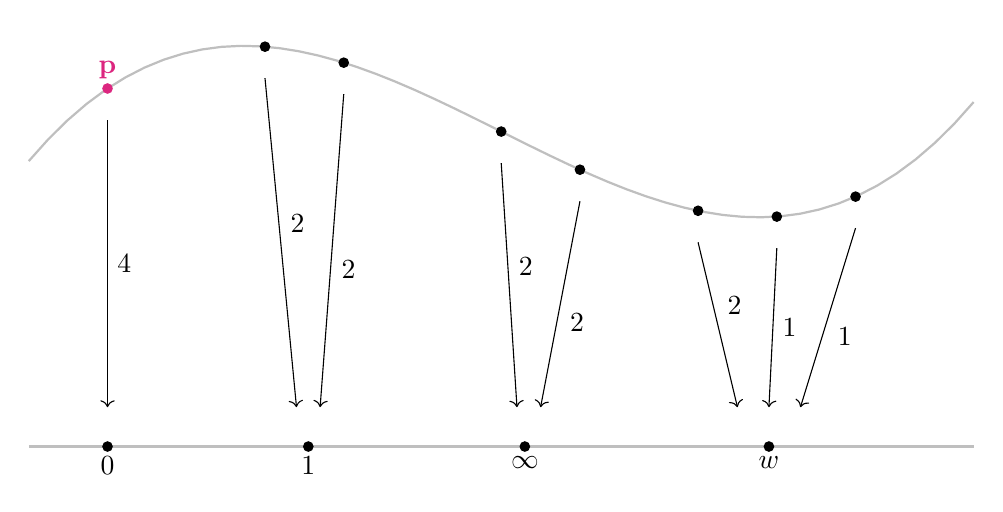
\begin{tikzpicture}
  \draw[domain=-6:6,samples=50,color=gray!50,thick] plot (\x, \x^3/64 - \x/2);
  \foreach \x/\p/\l in {-5/$\mathbf{p}$/4}
  {
    \filldraw[mypink] (\x,\x^3/64 - \x/2) circle (0.6mm) node[above] {\p};
    \draw[->] (\x,\x^3/64 - \x/2 - .4) to["$\l$"] (-5, -3.5);
  }
  \foreach \x/\p/\l in {-3//2, -2//2}
  {
    \filldraw[black] (\x,\x^3/64 - \x/2) circle (0.6mm) node[above] {\p};
    \draw[->] (\x,\x^3/64 - \x/2 - .4) to["$\l$"] (-1.7+.3*\x, -3.5);
  }
  \foreach \x/\p/\l in {0//2, 1//2}
  {
    \filldraw[black] (\x,\x^3/64 - \x/2) circle (0.6mm) node[above] {\p};
    \draw[->] (\x,\x^3/64 - \x/2 - .4) to["$\l$"] (.2+.3*\x, -3.5);
    }
  \foreach \x/\p/\l in {2.5//2, 3.5//1, 4.5//1}
  {
    \filldraw[black] (\x,\x^3/64 - \x/2) circle (0.6mm) node[above] {\p};
    \draw[->] (\x,\x^3/64 - \x/2 - .4) to["$\l$"] (2+.4*\x, -3.5);
    }

    \draw[domain=-6:6,samples=50,color=gray!50,thick] plot (\x, -4);
  \foreach \x/\q in {-5/$0$, -2.45/$1$, .3/$\infty$, 3.4/$w$}
    \filldraw[black] (\x,-4) circle (0.6mm) node[below] {\q};
\end{tikzpicture}

\label{fig:firsteg}
\end{figure}

The primary results we establish are as follows:
\begin{enumerate}
\item In Section 4, we study a generalization of Example~\ref{eg:firsteg}: given
  an even degree $d=2k$, a partition $\mu=(\mu_1,\dots,\mu_r)$ of $d$, and a generic
  $r$-pointed genus $1$ curve $(C,p_1,\dots,p_r)$, we ask how many maps
  $f:C\to\P^1$ exist with $f^{-1}(0)=\{p_1,\dots,p_r\}$, ramification index $\mu_i$
  at $p_i$, and ramification profiles $(2,\dots,2)$ over both $1$ and $\infty\in\P^1$.
  The answer to this ``even ramification'' problem is $3\cdot 2^{r-1}$, as
  proven in Corollary~\ref{cor:twos}. (In particular, there are $3$ maps of
  the kind considered in Example~\ref{eg:firsteg}.)
\item In Section 5, we study a different problem: given
  a degree $d$, a partition $\mu=(\mu_1,\dots,\mu_k)$ of $d$, multisets of positive integers $\a=\{a_1,\dots,a_r\}$ and $\b=\{b_1,\dots,b_s\}$,
  and a generic $(k+s)$-pointed genus $1$ curve $(C,p_1,\dots,p_k,P_1,\dots,P_s)$,
  we ask how many maps $f:C\to\P^1$ exist with $f^{-1}(0)=\{p_1,\dots,p_k\}$, ramification
  index $\mu_i$ at $p_i$, ramification index $b_i$ at $P_i$, and other (unmarked) points
  with ramification indices $a_1,\dots,a_r$.
  While we do not find a closed form solution, we develop recursive relations sufficient
  to calculate all such invariants in Theorems~\ref{thm:reduceb}, \ref{thm:reducea}, and \ref{thm:Sabbase}.
\item As a special case of point $2$: given a degree $d$ and a generic $d$-pointed genus $1$ curve $(C,x_1,\dots,x_d)$, we ask
  how many maps $f:C\to\P^1$ exist with $f^{-1}(0)=\{p_1,\dots,p_d\}$ and $d-2$ points in $C$ with ramification index $3$. Proposition~\ref{prop:deg4} shows that the answer is an explicit quartic in $d$, illustrating in this special case the usage of recurrence relations from Section 5.
  
  \end{enumerate}

Along the way we will demonstrate multiple techniques to calculate the enumerative
invariants of interest to us:
\begin{enumerate}
\item Direct evaluation, by using the line bundle characterization of maps to $\P^1$ to recast the problem as an enumerative question about subvarieties of projective space (explained in Sections \ref{section:direct1} and \ref{section:direct2});
\item Factoring covers as $C\to\P^1\to\P^1$, with the latter map of degree greater than $1$, where possible; we use this method in Section~\ref{section:comb};
  \item Solving the problem for a non-generic pointed {\it stable} curve. This method is not new; it was used originally in \cite{Cela} thanks to a technical result of \cite{Lian}, and is also used in \cite{Generalized}. Adapted to our context, it allows us to turn our central question into a combination of graph combinatorics and solving recurrence relations. In particular, we use this method heavily in Sections 4 and 5. (We outline this method in Section~\ref{section:admissible}.)
  \end{enumerate}

We note that the enumerative problem here is similar to a notion in the literature,
that of {\it generalized Tevelev degree} \cite{Generalized}. Like our problem, the notion
of generalized Tevelev degree turns the Hurwitz question on its head by fixing
a pointed source curve before counting possible covers of $\P^1$. However, there is a crucial difference
in that {\it both} a pointed source curve and certain points on the target $\P^1$ (where fibers will be ramified) are fixed. For instance:

\begin{eg}
  \label{eg:tevelev}
  Fix a generic genus $1$ curve $C$ with points $p_1,\dots,p_6\in C$. Also fix generic points
  $q_1,\dots,q_4\in\P^1$. We can consider degree $4$ maps $C\to\P^1$ where $p_1$ and $p_2$ are unramified points in the same fiber over $q_1$, $p_3$ and $p_4$ are unramified points in the same fiber over $q_2$, and $p_5$ and $p_6$ are ramified of index $2$ over the points $q_3$ and $q_4$ respectively.

  \begin{figure}[h]
  \caption{Illustration of the covers in Example~\ref{eg:tevelev}. Note that each depicted fiber has two unramified points not shown, and there are $5$ simply branched points not shown. Each pink, bolded point is fixed.}
  \centering
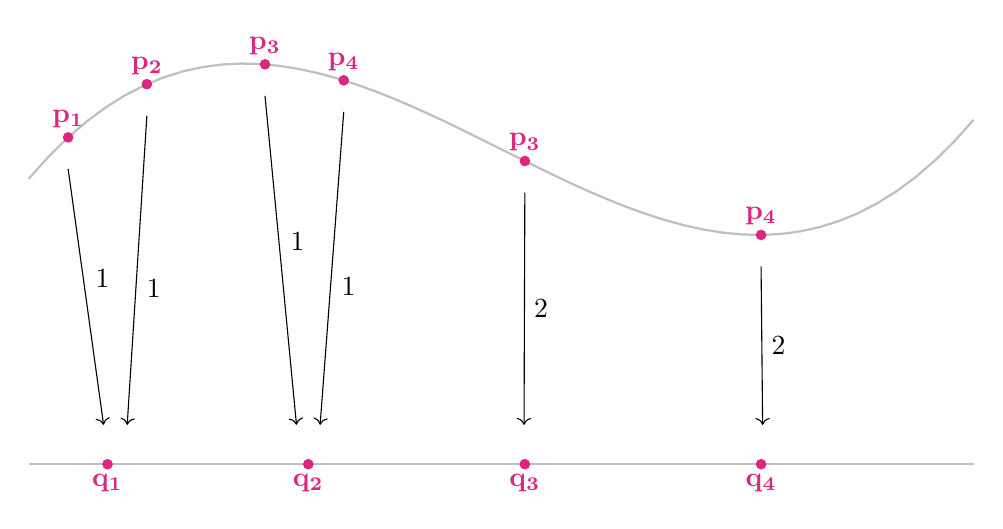
\begin{tikzpicture}
  \draw[domain=-6:6,samples=50,color=gray!50,thick] plot (\x, \x^3/64 - \x/2);
  \foreach \x/\p/\l in {-5.5/$\mathbf{p_1}$/1, -4.5/$\mathbf{p_2}$/1}
  {
    \filldraw[mypink] (\x,\x^3/64 - \x/2) circle (0.6mm) node[above] {\p};
    \draw[->] (\x,\x^3/64 - \x/2 - .4) to["$\l$"] (-3.4+.3*\x, -3.5);
  }
  \foreach \x/\p/\l in {-3/$\mathbf{p_3}$/1, -2/$\mathbf{p_4}$/1}
  {
    \filldraw[mypink] (\x,\x^3/64 - \x/2) circle (0.6mm) node[above] {\p};
    \draw[->] (\x,\x^3/64 - \x/2 - .4) to["$\l$"] (-1.7+.3*\x, -3.5);
  }
  \foreach \x/\p/\l in {0.3/$\mathbf{p_3}$/2}
  {
    \filldraw[mypink] (\x,\x^3/64 - \x/2) circle (0.6mm) node[above] {\p};
    \draw[->] (\x,\x^3/64 - \x/2 - .4) to["$\l$"] (.2+.3*\x, -3.5);
    }
  \foreach \x/\p/\l in {3.3/$\mathbf{p_4}$/2}
  {
    \filldraw[mypink] (\x,\x^3/64 - \x/2) circle (0.6mm) node[above] {\p};
    \draw[->] (\x,\x^3/64 - \x/2 - .4) to["$\l$"] (2+.4*\x, -3.5);
    }

    \draw[domain=-6:6,samples=50,color=gray!50,thick] plot (\x, -4);
  \foreach \x/\q in {-5/$\mathbf{q_1}$, -2.45/$\mathbf{q_2}$, .3/$\mathbf{q_3}$, 3.3/$\mathbf{q_4}$}
    \filldraw[mypink] (\x,-4) circle (0.6mm) node[below] {\q};
\end{tikzpicture}

\label{fig:tevelev}
\end{figure}

  In the notation of \cite{Generalized} we have $g=1$, $d=4$, $\ell=2$, $k=4$, $\mu_1=\mu_2=(1,1)$, $\mu_3=\mu_4=(2)$ and $n=6$. By Theorem 9 of that paper, the enumerative count is
  \[
  \text{Tev}_{1,2,(1,1),(1,1),(2),(2)}=2^1=2.
  \]
\end{eg}

\chapter{Problem Statement and General Approaches}

\section{Definitions}
Fix a positive integer $d$, a nonnegative integer $g$, ordered partitions $\sigma_1,\dots,\sigma_n$ of $d$, and subpartitions $\nu_1,\dots,\nu_n$ (i.e., $\nu_i$ is a subset of $\sigma_i$).

Let $\Hb_{g,\sigma}$ be the moduli space consisting of degree $d$ admissible covers $C\to X$ where $C$ is a genus $g$ prestable curve and $X$ is a genus $0$ prestable curve, marked points $p_{i,j}\in C$ for every $i\in\{1,\dots,n\}$ and
$j\leq \ell(\sigma_i)$, 
marked points $q_1,\dots,q_n\in X$ such that
the fiber over $q_i$ is $\{p_{i,1},\dots,p_{i,\ell(\sigma_i)}\}$ with
ramification profile $\sigma_i$, and the map is \'etale away from $q_1,\dots,q_n$ and any nodes of the target. Our situation is described in Figure \ref{fig:hurwitz}.

%TODO: something other than color, for accessibility?


Let $m=\sum\ell(\nu_i)$ and $N=\sum\ell(\sigma_i)$.
We have natural maps:
%TODO: make sure this will display next
\begin{figure}[h]
  \caption{Maps from the Hurwitz moduli space}
  \centering
  \[\begin{tikzcd}
	{\overline{\mathcal H}_{g,\sigma}} & {\overline{\mathcal M}_{g,N}} \\
	{\overline{\mathcal M}_{0,n}} & {\overline{\mathcal M}_{g,m}}
	\arrow["{\epsilon_g}", from=1-1, to=1-2]
	\arrow["{\epsilon_0}"', from=1-1, to=2-1]
	\arrow["{\pi_{\nu}}"', from=1-1, to=2-2]
	\arrow["\iota", from=1-2, to=2-2]
\end{tikzcd}\]
\label{fig:maps}
\end{figure}



Here $\pi_{\nu}$ remembers the source curve and the points corresponding to $\nu$; $\epsilon_0$ remembers the target with its marked
branch points; $\epsilon_g$ remembers the source curve and all points
corresponding to $\sigma$; and $\iota$ is the forgetful map, which forgets
the points of the source corresponding to $\sigma-\nu$ and stabilizes.



\begin{lem}
  \label{lem:dim}
  The source and target of $\pi_{\nu}$ are of the same dimension when $3g+m=n$,
  and thus if $\pi_{\nu}$ is finite this condition must hold.
\end{lem}
\begin{proof}
  By Hurwitz theory, we know that the map $\epsilon_0$ is finite, and so $\dim(\Hb_{\sigma,\mu})=n-3$. The map $\pi_{\nu}$ will be finite if and only if
  $\dim(\Hb_{\sigma,\mu})=\dim(\mb_{g,m})$, i.e.
  \[
  3g-3+m=n-3\iff 3g+m=n.
  \]
\end{proof}

\begin{figure}[h]
  \caption{Depiction of a Hurwitz cover with notation used in this thesis. Pink, bolded points are the ones fixed when counting $N_{g,\sigma,\nu}$.}
  \centering
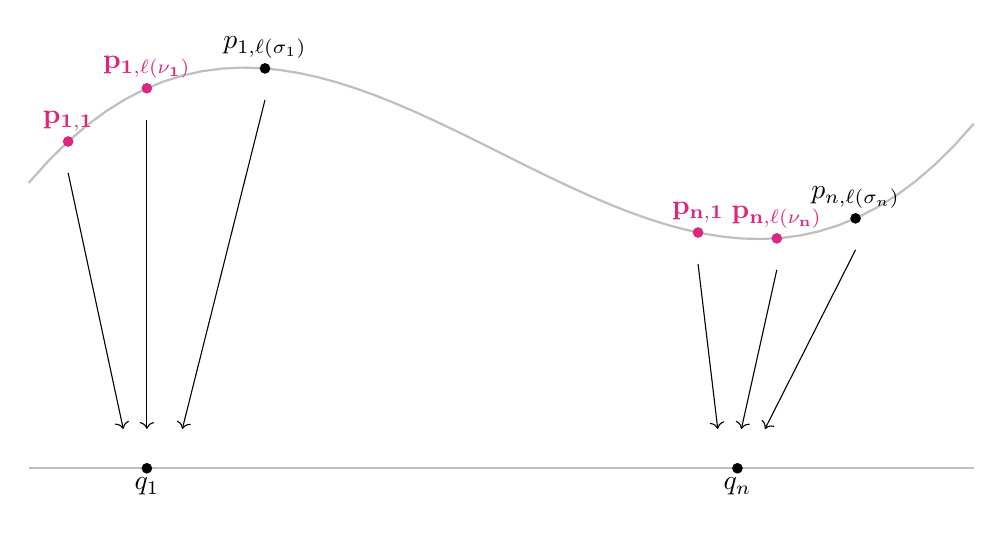
\begin{tikzpicture}
  \draw[domain=-6:6,samples=50,color=gray!50,thick] plot (\x, \x^3/64 - \x/2);
  \foreach \x/\p/\c/\l in {-5.5/$\mathbf{p_{1,1}}$/mypink/$\sigma_{1,1}$, -4.5/$\mathbf{p_{1,\ell(\nu_1)}}$/mypink/$\sigma_{1,\ell(\nu_1)}$, -3/$p_{1,\ell(\sigma_1)}$/black/$\sigma_{1,\ell(\sigma_1)}$}
  {
    \filldraw[\c] (\x,\x^3/64 - \x/2) circle (0.6mm) node[above] {\p};
    \draw[->] (\x,\x^3/64 - \x/2 - .4) -- (-3.15+.3*\x, -3.5);
    }
  \foreach \x/\p/\c in {2.5/$\mathbf{p_{n,1}}$/mypink, 3.5/$\mathbf{p_{n,\ell(\nu_n)}}$/mypink, 4.5/$p_{n,\ell(\sigma_n)}$/black}
  {
    \filldraw[\c] (\x,\x^3/64 - \x/2) circle (0.6mm) node[above] {\p};
    \draw[->] (\x,\x^3/64 - \x/2 - .4) -- (2+.3*\x, -3.5);
    }

    \draw[domain=-6:6,samples=50,color=gray!50,thick] plot (\x, -4);
  \foreach \x/\q in {-4.5/$q_1$, 3/$q_n$}
    \filldraw[black] (\x,-4) circle (0.6mm) node[below] {\q};
\end{tikzpicture}

\label{fig:hurwitz}
\end{figure}

When the condition of Lemma~\ref{lem:dim} is satisfied, we can define:
\begin{dfn}
  For a genus $g$, list of partitions $\sigma$ of the
  same positive integer $d$, and subpartitions $\nu$,
\[
W_{g,\sigma,\nu}=\deg(\pi_{\nu})
\]
where this is an orbifold degree.
\end{dfn}
In order to account for relabeling of marked points (any of the points $q_n$ with identical data, as well as any of the unmarked points in fibers with
identical data), we define
\[
N_{g,\sigma,\nu}=\frac{W_{g,\sigma,\nu}}{|\Aut(\sigma-\nu)|}
\]
where $\Aut(\sigma-\nu)$ denotes automorphisms of $\sigma_i-\nu_i$ for each $i$ together with automorphisms of $\{\sigma_i-\nu_i\}$, i.e.
\[
|\Aut(\sigma-\nu)|=|\Aut(\{(\sigma_i,\nu_i):1\leq i\leq n\})|\cdot \prod_i|\Aut(\sigma_i-\nu_i)|.
\]
\begin{eg}
  When $g=1$, $\sigma=((2,2),(3,1),(2,2),(2,1,1),(2,1,1))$ and $\nu=((2,2),\emptyset,\emptyset,\emptyset,\emptyset)$, we have
  \[
  N_{g,\sigma,\nu}=\frac{W_{g,\sigma,\nu}}{|\Aut(3,1)|\cdot |\Aut(2,2)|\cdot |\Aut(2,1,1)|^2\cdot |\Aut((3,1),(2,2),(2,1,1),(2,1,1))|}=\frac{W_{g,\sigma,\nu}}{1\cdot 2\cdot 2^2\cdot 2}
  \]
  Here $\Aut(\{x_1,\dots,x_k\})$ is the subgroup of $S_k$ fixing these elements.
  \end{eg}

One way to think about $N_{g,\sigma,\nu}$ is as follows: the map
$\pi_{\nu}:\Hb_{g,\sigma}\to\mb_{g,m}$ factors through
$\Hb_{g,\sigma}/\Aut(\sigma-\nu)$, and $N_{g,\sigma,\nu}$ is the degree of the map
\[
\Hb_{g,\sigma}/\Aut(\sigma-\nu)\to\mb_{g,m}.
\]

In many cases studied in this thesis, we will specialize to the case where $g=1$,
$\sigma_1=\nu_1=\mu$, and $\nu_3=\nu_4=\dots=\emptyset$.
\begin{dfn}
  We will write
\[
W_{\sigma_1,\dots,\sigma_n}(\mu)=W_{1,(\mu,\sigma_1,\dots,\sigma_n),(\mu,\emptyset,\dots,\emptyset)}
\]
for the relevant labeled invariant, and
\[
N_{\sigma_1,\dots,\sigma_n}(\mu)=N_{1,(\mu,\sigma_1,\dots,\sigma_n),(\mu,\emptyset,\dots,\emptyset)}
\]
for the unlabeled invariant.\end{dfn}
In particular,
\[
N_{\sigma_1,\dots,\sigma_n}(\mu)=\frac{W_{\sigma_1,\dots,\sigma_n}(\mu)}{|\Aut(\sigma_2,\dots,\sigma_n)|\cdot\prod_{i=2}^n|\Aut(\sigma_i)|}
\]
If $\mu,\sigma_1,\dots,\sigma_n$ do not have ramification sufficient to satisfy Riemann-Hurwitz,
we let \[N_{\sigma_1,\dots,\sigma_n}(\mu) = N_{\sigma_1,\dots,\sigma_n,(2,1^{d-2}),\dots}(\mu).\]
The primary task of this thesis is to understand the invariants $N_{\sigma_1,\dots,\sigma_n}(\mu)$
in some significant special cases.

\begin{eg}
  Consider the case where $d=2$, $n=1$, $\mu=\sigma_1=\sigma_2=\sigma_3=(2)$.
  We know that there is a unique map $(E,p)\to (\mathbb P^1,0)$ of the specified form
  up to automorphisms of $\P^1$,
  so
  \[
  N(2)=N_{(2),(2),(2)}(2)=1.
  \]
\end{eg}

\begin{eg}
  Consider the case where $g=0$, $\sigma=(\sigma_1,\sigma_2,\sigma_3)$ and $m=3$. In this case
  \[
  W_{0,\sigma,\nu}=\overline H(\sigma_1,\sigma_2,\sigma_3)
  \]
  where $\overline H$ is a marked Hurwitz number.
  \end{eg}

\section{Direct evaluation}
\label{section:direct1}
We can interpret $N_{\sigma_1,\dots,\sigma_n}(\mu)$ as follows.

Let $d>2$. Up to automorphisms of $\P^1$, a degree $d$ map $f:E\to\P^1$ corresponds to a degree $d$ line bundle $\mathcal L$ and a basepoint-free two-dimensional subspace $V\subset H^0(E,\mathcal L)$. By Riemann-Roch (\cite{Hartshorne}, p.\ 295), $\mathcal L$ gives an embedding $E\hookrightarrow\P(H^0(E,\mathcal L))\cong\P^{d-1}$, and a basepoint-free two-dimensional subspace $V\subset H^0(E,\mathcal L)$ corresponds to a well-defined composition
\[
E\hookrightarrow \P(H^0(E,\mathcal L))=\P(V\oplus V^{\perp})\dashrightarrow\P(V)\cong\P^1
\]
For the composition to be well-defined, $E$ should not intersect $\P(V^{\perp})$, a codimension 2 subspace of $\P(H^0(E,\mathcal L))$. Each fiber of the rational map
$\P(V\oplus V^{\perp})\dashrightarrow\P(V)$ is a hyperplane containing $\P(V^{\perp})$, and so the fibers of the map $E\to\P^1$ correspond to intersections $H\cap E$ where $H$ is some hyperplane containing $\P(V^{\perp})$. Thus, $N_{\sigma_1,\dots,\sigma_n}(\mu)$ can be determined by embedding $E$ in $\P^{d-1}$ via $\mathcal L=\mathcal O(\mu_{1}p_1+\dots+\mu_{\ell(\mu)}p_{\ell(\mu)})$ and counting the number of codimension 2 subspaces $\P(V^{\perp})\subset \P^{d-1}$ such that (a) $\P(V^{\perp})\cap E=\emptyset$, (b) $\P(V^{\perp})\subset H_0$ where $H_0\cap E=\mu_{1}p_1+\dots+\mu_{\ell(\mu)}p_{\ell(\mu)}$, (c) $\P(V^{\perp})\subset H_i$ where $H_i\cap E$ has shape $\sigma_i$, for $i=1,\dots,n$.

Note that if $\P(V^{\perp})$ is such a codimension 2 subspace corresponding to a map $f$, then $-\P(V^{\perp})$ (applying the involution on $E$, which extends to an automorphism of $\P(H^0(E,\mathcal L))$) is as well and corresponds to $x\mapsto f(-x)$.

\begin{eg}
  Let's compute $N_{(3)}(3)$. Embedding $E\hookrightarrow\P^2$ via $\mathcal L=\mathcal O(3p)$, we want to count the points $q\notin E$ such that
  $q\in\ell_0$ (the line at infinity) and $q\in\ell_1$, where $\ell_1\cap E=3r$ for some $r\neq p$ (we don't need to worry about the simple ramification, which
  is guaranteed). Since $q=\ell_0\cap\ell_1$ we just need to count lines $\ell_1$ with $\ell_1\cap E=3r$ for $r\neq p$; these are flex lines corresponding to nontrivial 3-torsion points, of which there are $3^2-1=8$. Therefore,
  \[
  N_{(3)}(3)=8.
  \]
\end{eg}
\begin{eg}
  Let's compute $N_{(3)}(2,1)$. If $\mathcal O(2p_1+p_2)=\mathcal O(3p_{\infty})$, then we can embed $E$ in $\P^2$ with $p_{\infty}$ as the point at infinity
  and let $\ell_0$ be a line such that $\ell_0\cap E=2p_1+p_2$. We want to count points $q\notin E$ with $q\in \ell_0$ and $q\in \ell_1$, where $\ell_1$ is a flex line. This again amounts to counting flex lines, so $N_{(3)}(2,1)=3^2=9$.

  For similar reasons, $N_{(3)}(1,1,1)=9$.
\end{eg}

Another way to count $N_{\sigma_1,\dots,\sigma_n}(\mu)$: note that $\{H:\P(V^{\perp})\subset H\}$ is a line in $\P(H^0(E,\mathcal L))^*$.
Let $X_{\mu}=\{H\in\P(H^0(E,\mathcal L))^*:H\cap E\text{ has shape }\mu\}$.
Counting the number of possibilities $\P(V^{\perp})$ amounts to counting lines $\ell\subset\P(H^0(E,\mathcal L))^*$ such that $H_0\in\ell$, $H_1,\dots,H_{n}\in\ell$ for distinct points $H_i\in X_{\mu_i}$, and $\P(V^{\perp})\cap E=H_0\cap H_1\cap E=\emptyset$.
Letting $\pi:\P^{d-1}\dashrightarrow \{\text{lines in $\P^{d-1}$ through $H_0$}\}=\P^{d-2}$ send $x$ to the line through $x$ and $H_0$, the idea is to count points in $\P^{d-2}$ whose fiber contains distinct points $H_i\in X_{\mu_i}$.

\begin{dfn}
  Assume $E\subset \P^{d-1}$. For any partition $\tau=(\tau_1,\dots,\tau_r)$ of $d$,
  \[
  X_{\tau}=\{H\in (\P^{d-1})^*:H\cap E=\tau_1x_1+\dots+\tau_rx_r\text{ for some }x_i\text{ not necessarily distinct}\}
  \]
\end{dfn}

Note that these subvarieties $X_{\tau}$ form a stratification of $(\P^{d-1})^*$,
with $\dim(X_{\tau})=\ell(\tau)-1$ and with
\[
X_{(\tau_1,\tau_2,\dots,\tau_r)}\subset X_{(\tau_1+\tau_2,\tau_3,\dots,\tau_r)}
\]
%(TODO: cite this stratification somewhere?)
We have an alternate interpretation, as well, of $X_{\tau}$ as the locus of effective divisors of shape $\tau$ (or a specialization of $\tau$) equivalent to $\mu_1p_1+\dots+\mu_kp_k$, or equivalently which are zero in the group law of $E$:
\[
X_{\tau}\cong\{(x_1^{\tau_1},\dots,x_r^{\tau_r})\in\text{Sym}^d(E):\tau_1x_1+\dots+\tau_rx_r=0\in E\}
\]


\begin{prop}
  \label{prop:direct}
  Fix $\mu=(\mu_1,\dots,\mu_k)$ a partition of $d$, and consider
  a generic $k$-pointed
  genus $1$ curve $(E,p_1,\dots,p_k)$ embedded in $\P^{d-1}$ with a hyperplane
  $H_0$ such that $H_0\cap E = \mu_1p_1+\dots+\mu_kp_k$.
  
  Let $\pi:(\P^{d-1})^*\dashrightarrow\{\text{lines in }(\P^{d-1})^*\text{ through }H_0\}\cong \P^{d-2}$. Then
  \[
  N_{\sigma_1,\dots,\sigma_n}(\mu)=\left|\left\{q\in\P^{d-2}-\bigcup_{i=1}^kB_i:\pi^{-1}(q)=\{H_1,\dots,H_n\}\text{ where }H_i\in X_{\sigma_i}\text{ are distinct}\right\}\right|
  \]
  where $B_i=\{\ell\subset(\P^{d-1})^*:H_0\in \ell\subset\{H:p_i\in H\}\}$ is a hyperplane in \[\{\text{lines in }(\P^{d-1})^*\text{ through }H_0\}\cong \P^{d-2}.\]
     (Note that if $\mu=(1,\dots,1)$, then $\pi$ is a projection onto a generic hyperplane.)
\end{prop}
\begin{proof}
  We know that $N_{\sigma_1,\dots,\sigma_n}(\mu)$ is the number of codimension $2$
  subspaces $\P(V^{\perp})\subset\P^{d-1}$ which do not intersect $E$, and which are contained in distinct $H_0,H_1,\dots,H_n$ where $H_i\in\sigma_i$. Such a subspace
  $\P(V^{\perp})$ can be written $\P(V^{\perp})=H_i\cap H_j$ for any distinct $i$
  and $j$.
  The locus of $H\in(\P^{d-1})^*$ containing
  a given subspace $\P(V^{\perp})$ of codimension $2$ is equivalent to a
  line in $(\P^{d-1})^*$, so we are interested in
  tuples of distinct hyperplanes $H_0,H_1,\dots,H_n$ which are collinear in
  $(\P^{d-1})^*$. The requirement that $\P(V^{\perp})=H_0\cap H_i$ does not intersect $E$ is equivalent to $H_i$ not containing any $p_1,\dots,p_k$, or that
  the line between $H_0$ and $H_i$ is not in any $B_1,\dots,B_k$.
\end{proof}

\begin{eg}
  We return to the computation of $N_{(3)}(3)=N_{(3),(2,1),(2,1)}(3)$. Let $(E,p)$
  be a generic elliptic curve in $\P^{d-1}=\P^2$; the map $\pi:(\P^2)^*\dashrightarrow \P^1$ is projection away from the line at infinity $\ell_{\infty}$.
  Here $X_{(3)}=\{\ell:\ell\cap E=3x\text{ for some }x\}$ consists of the flex lines to $E$ (of which there are $3^2=9$ corresponding to $3$-torsion points, and one of which is $\ell_{\infty}$), while $X_{(2,1)}\subset (\P^2)^*$ is the dual curve of $E$ mapping surjectively onto $\P^1$ under $\pi$. We know that $|\pi(X_{(3)})|=8$ (since $\ell_{\infty}$ is not in the domain of $\pi$), so $N_{(3)}(3)=|\pi(X_{(3)}|=8$.
  \end{eg}


\section{Low-dimensional examples}

In this section, we use
Macaulay2 calculations to
compute $N_{\sigma_1,\dots,\sigma_n}(\mu)$ in a couple degree $4$ cases
using Proposition~\ref{prop:direct}; the
code and some details are in Appendix~\ref{appendix:code}) We provide tables with values of some invariants in degrees $3$, $4$, and $5$.

Let $d=4$, and consider a generic elliptic curve $(E,p)$ embedded in $\P^3$ via
$\mathcal L=\mathcal O(4p)$. We have a stratification of $(\P^3)^*$:

\begin{figure}[h]
  \caption{Stratification of $(\P^3)^*$ by shape of pullback to $E$}
  \centering
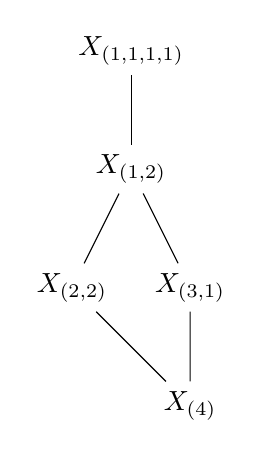
\begin{tikzpicture}
  \node {$X_{(1,1,1,1)}$}
  child {node {$X_{(1,2)}$}
    child {node[name=A] {$X_{(2,2)}$}}
    child {node {$X_{(3,1)}$}
      child {node[name=B] {$X_{(4)}$}}}};
  \draw (A) edge (B);
\end{tikzpicture}
\end{figure}

First, note that \[X_{(2,2)}\cong\{(x,y)\in E^2:2x+2y=0\}/S_4=\{(x,y)\in E^2:x+y\text{ is 2-torsion}\}/S_2\]
so $X_{(2,2)}$ is a disjoint union of four curves each corresponding to a 2-torsion point $t_i$:
\[
C_i=\text{image}(f_i:E\hookrightarrow(\P^3)^*),\ f_i(x)=H\text{ where }H\cap E=2x+2(t_i-x)
\]
Note that $f_i$ is 2-to-1 ($x$ and $t_i-x$ are in the same fiber), so $C_i\cong E/S_2\cong\P^1$. See Listing~\ref{code:X22} for the computation in Macaulay2 to compute $X_{(2,2)}$; it turns out that each $C_i$ is a plane conic. Consequently,
we know for instance that
\[
N_{(2,2),(2,2)}(1,1,1,1)=\#\left(\bigcup_{i\neq j}\pi(C_i)\cap \pi(C_j)\right)=\binom 42\cdot 2^2=24
\]
where $\pi$ is a generic projection $\P^3\dashrightarrow\P^2$, as in
Proposition~\ref{prop:direct}.

The case $N_{(3,1),(3,1)}(1,1,1,1)$ is of interest; it corresponds to counting
the number of fibers of a generic projection $\pi:\P^3\dashrightarrow\P^2$
containing multiple points of $X_{(3,1)}$. Equivalently this is the number of
double fibers of the map $X_{(3,1)}-\{H_0\}\to \pi(X_{(3,1)}-\{H_0\})=Y_{(3,1)}$, or the number of nodes of $Y_{(3,1)}$.

Since the projection in this case is generic, $\text{deg}(Y_{(3,1)})=\text{deg}(X_{(3,1)})=12$ (by results of Listing~\ref{code:X31}, or by Lemma~\ref{lemma:degree}) and the degree-genus formula (\cite{Hartshorne} p.\ 54, Exercise 7.2) tells us that the arithmetic genus
of $Y_{(3,1)}$ is
\[
g_a=\frac{(11)(10)}{2}=55
\]
The geometric genus of $X_{(3,1)}$ is $1$ and it has $16$ cusps,
so the number of nodes of $Y_{(3,1)}$ is% (TODO: really understand)
\[
N_{(3,1),(3,1),(1,1,1,1)}=55-16-1=38
\]
In principle one could hope that the method of this example ---
computing the degree of $X_{(3,1)}$ and relating degree, genus, and
number of singularities
--- is generalizable to tackle $N_{\tau,\tau}(\mu)$. However, the degree-genus
formula is critical here and it is not obvious how to replace this tool in higher dimensions.

We provide the following tables of invariants in degrees $d=3$, $d=4$, and $d=5$:


  \begin{table}[ht]
    \caption{Table of invariants for $n=3$.}
    \centering
    ~\\
  \begin{tabular}{|l|r|}
    \hline
$\mu$           & ${N_{(3)}(\mu)}$ \\ \hline
$3$ & 8                                           \\ \hline
$2,1$                   & $9$                              \\ \hline
$1,1,1$                 & $9$ \\ \hline
\end{tabular}
\end{table}

  \begin{table}[h]
    \caption{Table of invariants for $n=4$.}
    \centering
    ~\\
\begin{tabular}{|l|l|l|l|l|}
\hline
$\mu$             & $N_{(4)}(\mu)$ & $N_{(3,1),(2,2)}(\mu)$ & $N_{(2,2),(2,2)}(\mu)$ & $N_{(3,1),(3,1)}(\mu)$ \\ \hline
{4} & {15} & {18}        & {3}         & {20}        \\ \hline
3,1                     & {16} & {32}        & {6}         & {28}        \\ \hline
2,2                     & {16} & {18}        & {6}         & {36}        \\ \hline
2,1,1                   & {16} & {36}        & {12}        & {37}        \\ \hline
1,1,1,1                 & {16} & {48}        & {24}        & {38}        \\ \hline
\end{tabular}
\end{table}

  \begin{table}[h]
    \caption{Table of invariants for $n=5$.}
    \centering
    ~\\
\begin{tabular}{|l|l|l|}
\hline
$\mu$             & $N_{(4,1),(3,1,1)}(\mu)$ & $N_{(3,1,1),(3,1,1),(3,1,1)}(\mu)$ \\ \hline
{5} & {72}                                       & {16}                    \\ \hline
4,1                     & {95}                                       & {36}                    \\ \hline
3,2                     & {118}                                      & {56}                    \\ \hline
3,1,1                   & {120}                                      & {64}                    \\ \hline
2,2,1                   & {136}                                      & {92}                    \\ \hline
2,1,1,1                 & {138}                                      & {101}                   \\ \hline
1,1,1,1,1               & {140}                                      & 110                                        \\ \hline
\end{tabular}
\end{table}

\chapter{Admissible Covers}
\label{section:admissible}

Up to now, we have computed our invariants of interest by direct evaluation in some
low-dimensional cases, including
by use of Macaulay2. 
In this chapter we explain a more systematic and general
known method in the literature that we will use
to recursively compute invariants $W_{g,\sigma,\nu}$. Cela and Lian use this method to prove Proposition 6 in \cite{Generalized}, relying on a result from an earlier paper of Lian's \cite{Lian}. We begin by motivating the method, and then illustrate the use of the method as adapted to the specific context of this thesis.

Recall that $W_{g,\sigma,\nu}$ is the degree of the map $\pi_{\nu}:\Hb_{g,\sigma}\to\mb_{g,m}$
where $\sum\ell(\nu_i)=m$; our enumerative interpretation is that, for a fixed general $m$-pointed genus $g$ curve $(C,p_1,\dots,p_m)$, $W_{g,\sigma,\nu}$ counts the number of Hurwitz covers of the correct form with source $(C,p_1,\dots,p_m)$. One can hope (and we will confirm) that the same is roughly true for
a specific $m$-pointed genus $g$ {\it stable} curve lying in a suitable boundary divisor of $\mb_{g,m}$.

We first begin with a rough illustration of what we intend to do.

\begin{eg}
  \label{eg:fourtorsion}
  Suppose we are interested in calculating $W_{(3),(2,1),(2,1),(2,1)}(2,1)$, the degree of the map
  \[
  \pi:\Hb_{1,\sigma}\to\mb_{1,2}
  \]
  
  Let $A$ be the following stable graph:

  \begin{figure}[h]
    \caption{Stable graph consisting of a genus $1$ vertex connected to a genus $0$ vertex, with two legs on the
  genus $0$ vertex}
    \centering
  \begin{tikzpicture}[thick]

  \matrix[amat,nodes=fsnode] (mat1) {$1$\\};

 \matrix[amat,right=4cm of mat1,nodes=ssnode] (mat2) {$0$\\};

 \draw  (mat1-1-1) edge (mat2-1-1);
 
  % draw legs for right side
 \draw  (mat2-1-1) -- +(30:.58) node[anchor=west] {$p_{1,1}$}
 (mat2-1-1) -- +(330:.58) node[anchor=west] {$p_{1,2}$};

  \end{tikzpicture}
  \end{figure}
  

  Intuitively we want to count covers from a generic stable curve with dual graph $A$ to a genus $0$
  curve, such that $p_{1,1}$ and $p_{1,2}$ are in the same fiber (with ramification indices $2$ and $1$),
  and there is marked ramification elsewhere with ramification profiles $(3),(2,1),(2,1),(2,1)$.
  Remembering the marked points, the source should be a stable curve in $\mb_{1,9}$ with dual graph $\hat A$, where $\hat A$
  becomes $A$ after applying a forgetful map.

  One possible graph $\hat A_1$ is the source of a type of admissible cover in $\Hb_{1,\sigma}$:

  \begin{figure}[h]
    \caption{A graph $\hat A_1$ obtained from $A$ by putting $p_{5,1}$ and $p_{5,2}$ on the genus $0$ component and other
  marked points on the genus $1$ component}
    \centering
                  \begin{tikzpicture}[thick]

  \matrix[amat,nodes=fsnode] (mat1) {$1$\\};

    \matrix[dmat,left=1.3cm of mat1] (degrees1) {$3$\\};


 \matrix[amat,right=4cm of mat1,nodes=ssnode] (mat2) {$0$\\};

 \matrix[dmat,right=1.3cm of mat2] (degrees2) {$3$\\};

 \draw  (mat1-1-1) edge["$3$"] (mat2-1-1);

  % draw legs for left side
 \draw (mat1-1-1) -- +(45:.58) node[anchor=west] {$p_{2,1}$}
 (mat1-1-1) -- +(245:.58) node[anchor=north] {$p_{3,1}$}
 (mat1-1-1) -- +(305:.58) node[anchor=north] {$p_{3,2}$}
 (mat1-1-1) -- +(160:.58) node[anchor=east] {$p_{4,1}$}
 (mat1-1-1) -- +(190:.58) node[anchor=east] {$p_{4,2}$};
%  (mat1-1-1) -- +(95:.58) node[anchor=south] {$p_{5,1}$}
% (mat1-1-1) -- +(125:.58) node[anchor=south] {$p_{5,2}$};

 % draw legs for right side
 \draw  (mat2-1-1) -- +(10:.58) node[anchor=west] {$p_{1,1}$}
 (mat2-1-1) -- +(345:.58) node[anchor=west] {$p_{1,2}$}
 (mat2-1-1) -- +(50:.58) node[anchor=south] {$p_{5,1}$}
 (mat2-1-1) -- +(90:.58) node[anchor=east] {$p_{5,2}$};

                  \end{tikzpicture}
                  \end{figure}

                  Another possible graph $\hat A_2$
                  is the source of another type of admissible cover in $\Hb_{1,\sigma}$ (we omit the target, consisting of a blue and an orange genus $0$ vertex with one edge between them):

                  \begin{figure}[h]
                    \caption{A graph $\hat A_2$ obtained from $A$ by putting $p_{2,1}$ on the genus $0$ component
                  and the other marked points on the genus $1$ component,}
                    \centering
                                    \begin{tikzpicture}[thick]

                                      \matrix[amat,nodes=fsnode] (mat1) {$1$\\
                                      $0$\\};

  \matrix[dmat,left=1cm of mat1] (degrees1) {$2$\\
  $1$\\};


 \matrix[amat,right=4cm of mat1,nodes=ssnode] (mat2) {$0$\\};

 \matrix[dmat,right=1cm of mat2] (degrees2) {$3$\\};

 \draw  (mat1-1-1) edge["$2$"] (mat2-1-1)
 (mat1-2-1) edge["$1$"] (mat2-1-1);

  % draw legs for left side
 \draw (mat1-1-1) -- +(35:.58) node[anchor=west] {$p_{5,1}$}
 (mat1-2-1) -- +(35:.58) node[anchor=west] {$p_{5,2}$}
 (mat1-1-1) -- +(220:.58) node[anchor=north] {$p_{3,1}$}
 (mat1-2-1) -- +(220:.58) node[anchor=north] {$p_{3,2}$}
 (mat1-1-1) -- +(165:.58) node[anchor=east] {$p_{4,1}$}
 (mat1-2-1) -- +(165:.58) node[anchor=east] {$p_{4,2}$};

 % draw legs for right side
 \draw  (mat2-1-1) -- +(10:.58) node[anchor=west] {$p_{1,1}$}
 (mat2-1-1) -- +(345:.58) node[anchor=west] {$p_{1,2}$}
 (mat2-1-1) -- +(50:.58) node[anchor=south] {$p_{2,1}$};

                                    \end{tikzpicture}
                                    \end{figure}

                                    We hope that $W_{(3),(2,1),(2,1),(2,1)}(2,1)$ can be expressed
                                    as a sum of terms corresponding to these kinds of
                                    admissible covers:

                                    There are three graphs similar to $\hat A_1$, corresponding to a choice of $i\in\{3,4,5\}$ for which $p_{i,1}$ and $p_{i,2}$ appear on the genus $0$ component. The contribution from each graph should be a product
                                    \[
                                    W_{(3),(2,1),(2,1)}(3)\cdot \overline H((3),(2,1),(2,1))=W_{(3),(2,1),(2,1)}(3)\cdot 1=2N_{(3),(2,1),(2,1)}(3)=2\cdot 8=16
                                    \]
                                    There is only a single graph like $\hat A_2$,
                                    and its contribution is
                                    \[
                                    W_{(2),(2),(2)}(2)\cdot \overline H((3),(2,1),(2,1))=3!\cdot N_{(2),(2),(2)}(2)\cdot 1=6
                                    \]
                                    Therefore our expectation is that
                                    \[
                                    W_{(3),(2,1),(2,1),(2,1)}(2,1)=3\cdot 16+6=54\implies N_{(3),(2,1),(2,1),(2,1)}(2,1)=\frac{54}{3!}=9.
                                    \]
  \end{eg}

                \section{Setup}

                We now turn to a general explanation of this technique loosely applied in the example above, and in following \cite{Generalized} we will write an explicit application of the technique to our specific invariants.
                


Let $A$ be a stable graph
corresponding to a boundary stratum in $\mb_{g,m}$.
Following Proposition 3.2 of \cite{Lian}, we have a commutative diagram
\[\begin{tikzcd}
\amalg \mathcal H_{(\Gamma,\Gamma')} & \Hb_{g,\sigma} \\
\amalg \mb_{\hat A} & \mb_{g,N} \\
	\mb_A & \mb_{g,m}
	\arrow[from=1-1, to=1-2]
	\arrow[from=1-1, to=2-1, "\amalg \phi_{(\Gamma,\Gamma')}"]
        \arrow[from=2-1, to=3-1]
	\arrow[from=1-2, to=2-2]
	\arrow[from=2-1, to=2-2]
        \arrow[from=2-2, to=3-2]
        \arrow[from=3-1, to=3-2, "\xi_A"]
        \arrow[from=1-2, to=3-2, bend left=52, "\pi_{\nu}"]
        \arrow[from=1-1, to=3-1, bend right=52, "\phi"]
\end{tikzcd}\]

Here the index set of the top left object
consists of pairs $(\Gamma,\Gamma')$
where $\Gamma$ and $\Gamma'$ are stable graphs (the latter being genus $0$), $\Gamma\to\Gamma'$ is an admissible cover of stable graphs, $\Gamma$
comes with a chosen $\hat A$-structure (i.e., a specialization to $\hat A$),
and $\hat A$ is any stable graph reducing to $A$ under the forgetful map.
The index set of $\amalg\overline{\mathcal M}_{\hat A}$ consists of
all stable graphs reducing to $A$ under the forgetful map.

The outside square is Cartesian on the level of closed points. By
Proposition 3.3 of \cite{Lian}, if $\mathcal H_{(\Gamma,\Gamma')}$ is of
expected dimension, its contribution to $\xi_A^*(\pi_{\nu})_*([\Hb_{g,\sigma}])$
is a nonzero multiple of $\phi_*([\mathcal H_{(\Gamma,\Gamma')}])$ on $\overline{\mathcal M}_A$, and in fact the coefficient is given by the product of edges contracted in the $A$-structure of $\Gamma$ divided by the size of the automorphism group.% (TODO: why?).

\begin{thm}
  \label{thm:admissible}
  If $A$ is a stable graph corresponding to a boundary divisor in $\mb_{g,m}$, then
  \[
  \frac 1{|\Aut(A)|}W_{g,\sigma,\nu}=\sum_{\hat A\rightsquigarrow A}\sum_{(\Gamma,\Gamma')}\frac 1{|\Aut(\Gamma)|}c_{\Gamma}W_{(\Gamma,\Gamma')}
  \]
  where $\hat A$ becomes $A$ after forgetting points, $\Gamma$ is a stable graph with a chosen $\hat A$-structure and an admissible
  cover to $\Gamma'$ a stable genus $0$ graph with one edge, $c_{\Gamma}$ is the
  product of contracted edges in the $\hat A$-structure, and
  $W_{(\Gamma,\Gamma')}$ is a product of terms $W_{g',\sigma',\nu'}$ corresponding to each vertex of $\Gamma$.
\end{thm}

\begin{proof}
  Note that
  \[
  \xi_A^*(\pi_{\nu})_*([\mathcal H_{g,\sigma,\nu}]) =
  \xi_A^*(W_{g,\sigma,\nu}[\mb_{g,m}])=
  W_{g,\sigma,\nu}[\mb_A]
  \]
  Therefore, $W_{g,\sigma,\nu}$ is a sum of
  terms $\frac 1{|\Aut(\Gamma)|}c_{\Gamma}W_{(\Gamma,\Gamma')}$, for
  any $(\Gamma,\Gamma')$ such that
  $\mathcal H_{(\Gamma,\Gamma')}\to\mb_A$
  is dominant.

  We have a natural map $\mathcal H_{(\Gamma,\Gamma')}\to \mb_{\Gamma'}$ remembering the target, which is finite by Hurwitz theory. Therefore,
  \[
  \dim(\mathcal H_{(\Gamma,\Gamma')})=\dim(\mb_{\Gamma'})
  \]
  For $\mathcal H_{(\Gamma,\Gamma')}\to\mb_A$ to be
  dominant means therefore that
  \[
  \dim(\mb_{\Gamma'})=\dim(\mb_A)=
  \dim(\mb_{g,m})-1=\dim(\mb_{0,n})-1
  \]
  or equivalently that $\Gamma'$ has a single edge.
\end{proof}

\section{Genus reduction}

We can apply this technique to compute invariants $W_{\sigma_1,\dots,\sigma_n}(d)$ by reduction to
genus $0$ invariants, and illustrate with the following example.

\begin{eg}
  \label{eg:genusreduction}
  Suppose we are interested in calculating $W_{(4),(2,1,1),(2,1,1)}(4)$, the number of degree $4$ covers from a fixed elliptic curve $(E,p_1)$ to $\P^1$ with full ramification over $p_1$ and another point, with ramification points labeled.
  
  Let $A$ be a stable graph consisting of a single genus $0$ vertex with
  a loop and a leg labeled $p_{1,1}$; and let $\hat A$ be a graph with
  additional legs corresponding to the other fibers of ramification.

  While no such admissible cover
  can have actual source of the form described by $\hat A$ (due to the loop), there are in fact
  covers whose source {\it stabilizes} to the kind we want.
  Consider the following picture:

  \begin{figure}[h]
    \caption{A stable graph $\Gamma$ specializing to $\hat A$}
    \centering
              \begin{tikzpicture}[thick]

  \matrix[amat,nodes=fsnode] (mat1) {$0$\\};

 \matrix[amat,right=4cm of mat1,nodes=ssnode] (mat2) {$0$\\};

 \draw  (mat1-1-1) edge[bend left] (mat2-1-1)
 (mat1-1-1) edge[bend right] (mat2-1-1);

  % draw legs for left side
 \draw (mat1-1-1) -- +(95:.58) node[anchor=south] {$p_{1,1}$}
 (mat1-1-1) -- +(215:.58) node[anchor=east] {$p_{3,1}$}
 (mat1-1-1) -- +(245:.58) node[anchor=north] {$p_{3,2}$}
 (mat1-1-1) -- +(285:.58) node[anchor=west] {$p_{3,3}$};

 % draw legs for right side
 \draw  (mat2-1-1) -- +(60:.58) node[anchor=west] {$p_{2,1}$}
 (mat2-1-1) -- +(305:.58) node[anchor=north] {$p_{4,1}$}
 (mat2-1-1) -- +(330:.58) node[anchor=west] {$p_{4,2}$}
 (mat2-1-1) -- +(360:.58) node[anchor=west] {$p_{4,3}$};

              \end{tikzpicture}
              \end{figure}

  Note that $\Gamma$ can specialize to
  $\hat A$ in two ways, by contracting either of
  the two edges; each corresponds to a choice of $\hat A$-structure
  as defined in \cite{Schmitt}.
  In the sense of Definition 2.10 from \cite{Lian}, there is an admissible cover of stable graphs $\Gamma\to\Gamma'$ depicted as follows where $a+b=4$:

  \begin{figure}[h]
    \caption{First admissible cover $\Gamma\to\Gamma'$}
    \centering
                \begin{tikzpicture}[thick]

  \matrix[amat,nodes=fsnode] (mat1) {$0$\\};

    \matrix[dmat,left=1cm of mat1] (degrees1) {$4$\\};


 \matrix[amat,right=4cm of mat1,nodes=ssnode] (mat2) {$0$\\};

 \matrix[dmat,right=1cm of mat2] (degrees2) {$4$\\};

 \draw  (mat1-1-1) edge[bend left,"$a$"] (mat2-1-1)
 (mat1-1-1) edge[bend right,"$b$"] (mat2-1-1);

  % draw legs for left side
 \draw (mat1-1-1) -- +(125:.58) node[anchor=south] {$p_{1,1}$}
 (mat1-1-1) -- +(170:.58) node[anchor=east] {$p_{3,1}$}
 (mat1-1-1) -- +(195:.58) node[anchor=east] {$p_{3,2}$}
 (mat1-1-1) -- +(215:.58) node[anchor=east] {$p_{3,3}$};

 % draw legs for right side
 \draw  (mat2-1-1) -- +(30:.58) node[anchor=west] {$p_{2,1}$}
  (mat2-1-1) -- +(305:.58) node[anchor=north] {$p_{4,1}$}
 (mat2-1-1) -- +(330:.58) node[anchor=west] {$p_{4,2}$}
 (mat2-1-1) -- +(360:.58) node[anchor=west] {$p_{4,3}$};

                \end{tikzpicture}
                \end{figure}

                The contribution of such $(\Gamma,\Gamma')$ is
                \[
                \frac 1{|\Aut(\Gamma)|}c_{\Gamma}W_{(\Gamma,\Gamma')}=\frac 1{|\Aut(a,b)|}\cdot 4\cdot \overline H((4),(a,b),(2,1,1))\cdot \overline H((4),(a,b),(2,1,1))
                \]
                When $(a,b)=(2,2)$ this is
                \[
                \frac 12\cdot 4\cdot 2\cdot 2=8
                \]
                and when $(a,b)=(3,1)$ this is
                \[
                1\cdot 4\cdot 2\cdot 2=16.
                \]
                There are similar choices of $(\Gamma,\Gamma')$ where the components of $q_3$ and
                $q_4$ are swapped,
                yielding a cumulative sum of $2\cdot (8+16)=48$.

                The other type of cover $\Gamma\to\Gamma'$ to consider can be depicted as follows:

                \begin{figure}[h]
                  \caption{Second admissible cover $\Gamma\to\Gamma'$}
                  \centering
                                \begin{tikzpicture}[thick]

  \matrix[amat,nodes=fsnode] (mat1) {$0$\\};

    \matrix[dmat,left=1cm of mat1] (degrees1) {$4$\\};


    \matrix[amat,right=4cm of mat1,nodes=ssnode] (mat2) {$0$\\
      $0$\\
    $0$\\};

 \matrix[dmat,right=1cm of mat2] (degrees2) {$2$\\
   $1$\\
 $1$\\};

 \draw  (mat1-1-1) edge[bend left,"$1$"] (mat2-1-1)
 (mat1-1-1) edge["$1$"] (mat2-1-1)
 (mat1-1-1) edge["$1$"] (mat2-2-1)
 (mat1-1-1) edge["$1$"] (mat2-3-1);

  % draw legs for left side
 \draw (mat1-1-1) -- +(125:.58) node[anchor=south] {$p_{1,1}$}
 (mat1-1-1) -- +(225:.58) node[anchor=east] {$p_{2,1}$};

 % draw legs for right side
 \draw  (mat2-1-1) -- +(30:.58) node[anchor=west] {$p_{3,1}$}
 (mat2-2-1) -- +(30:.58) node[anchor=west] {$p_{3,2}$}
 (mat2-3-1) -- +(30:.58) node[anchor=west] {$p_{3,3}$}
 (mat2-1-1) -- +(330:.58) node[anchor=west] {$p_{4,1}$}
 (mat2-2-1) -- +(330:.58) node[anchor=west] {$p_{4,2}$}
 (mat2-3-1) -- +(330:.58) node[anchor=west] {$p_{4,3}$};


                                \end{tikzpicture}
                                \end{figure}

                                There are two choices for placement of $p_{3,2}$ and $p_{4,2}$
                                and two automorphisms of the graph
                                (swapping the two top edges), so
                                the contribution
                                is
                                \begin{align*}
                                  2\cdot \frac 1{|\Aut(\Gamma)|}c_{\Gamma}W_{(\Gamma,\Gamma')}&=2\cdot\frac 12\cdot 2\cdot \overline H((4),(4),(1,1,1,1))\cdot \overline H((2),(2),(1,1)) \\
                                  &=2\cdot 6\cdot 1\\
                                  &=12
                                \end{align*}
                                Combining our results,
                                \begin{align*}
                                  \frac 12W_{(4),(2,1,1),(2,1,1)}(4)=48+12=60&\implies W_{(4),(2,1,1),(2,1,1)}(4)=120 \\
                                  &\implies N_{(4),(2,1,1),(2,1,1)}(4)=\frac{120}{2^3}=15
                                \end{align*}
                                This matches our expectation, since $N_{(4),(2,1,1),(2,1,1)}(4)$ counts
                                nontrivial $4$-torsion points of an elliptic curve.
                                
\end{eg}

In general, any invariant $W_{\sigma_1,\dots,\sigma_n}(d)$ can be computed via this method, using the
same graph $A$ in this example and reducing to genus $0$ invariants (which will all be marked
Hurwitz numbers). One can also apply genus reduction for any
invariant $W_{\sigma_1,\dots,\sigma_n}(\mu)$ with $\ell(\mu)\geq 2$, although in
this case we will end up with enumerative counts in genus $0$ that
are more complicated than Hurwitz numbers.

  \section{Merging two points}

  In the case where $\ell(\mu)\geq 2$, we can consider the following graph $A$:

  \begin{figure}[h]
    \caption{Graph $A$ with two marked points on a genus $0$ vertex and all others on a genus $1$ vertex}
    \centering
  \begin{tikzpicture}[thick]

  \matrix[amat,nodes=fsnode] (mat1) {$1$\\};

 \matrix[amat,right=4cm of mat1,nodes=ssnode] (mat2) {$0$\\};

 \draw  (mat1-1-1) edge (mat2-1-1);

  % draw legs for left side
 \draw (mat1-1-1) -- +(165:.58) node[anchor=east] {$p_{1,3}$}
 (mat1-1-1) -- +(225:.58) node[anchor=north] {$\dots$}
 (mat1-1-1) -- +(285:.58) node[anchor=north] {$p_{1,\ell(\mu)}$};

 % draw legs for right side
 \draw  (mat2-1-1) -- +(60:.58) node[anchor=west] {$p_{1,1}$}
 (mat2-1-1) -- +(330:.58) node[anchor=west] {$p_{1,2}$};

  \end{tikzpicture}
  \end{figure}

                By applying the theorem to this graph, we can compute the value of
                $W_{\sigma_1,\dots,\sigma_n}(\mu)$ by reduction to marked Hurwitz
                numbers and terms of the form
                $W_{\tau_1,\dots,\tau_m}(\mu')$ where $\ell(\mu')<\ell(\mu)$, for instance
                in the first example of this section.
                The base case where $\ell(\mu)=1$ can be solved via genus reduction.
                In principle, this gives us a complete (albeit potentially combinatorially difficult) method to compute any invariant $W_{\sigma_1,\dots,\sigma_n}(\mu)$.

                More generally, we can use the theorem to compute $W_{g,\sigma,\nu}$ when $m=\sum\limits_{i=1}^n\ell(\nu_i)\geq 2$, by letting $A$ be a graph with a genus $g$ vertex attached to a genus $0$ vertex, and two of the
                marked points on the genus $0$ vertex. The following lemma will be useful:

                \begin{lem}
                  \label{lem:branchpoints}
                  Letting $A$ be as above, in Theorem~\ref{thm:admissible}, every admissible cover of graphs $\Gamma\to\Gamma'$ where $\Gamma$ contains a genus $g$ vertex (guaranteed when $g=1$) has precisely $2$ branch points
                  whose fiber does not intersect the genus $g$ vertex.
                \end{lem}

                \begin{proof}
                  Let $\Gamma\to\Gamma'$ be an admissible cover of graphs where $\Gamma$ comes with a $\hat A$-structure and $\hat A$ specializes to $A$, and assume $\Gamma$ has a genus $g$ vertex $v$.
                  Then $\Hb_{(\Gamma,\Gamma')}$ has a factor $\Hb_{v}$ corresponding to the vertex $v$,
                  and there is a finite map $\Hb_{v}\to\mb_{g,m-1}$ which recalls
                  the vertex $v$ along with the $m-2$ fixed points on the genus $g$ vertex of $A$ and
                  the point corresponding to the node of $A$. Thus,
                  \[
                  \dim(\Hb_v)=\dim(\mb_{g,m-1})=3g-3+m-1
                  \]
                  By Lemma~\ref{lem:dim}, $\dim(\Hb_v)=n-4$. There is also a finite morphism
                  $\Hb_v\to\mb_{0,k+1}$ where $k$ is the number of proper branch points from this
                  component (and thus $k+1$ is the number of branch points including the node), so
                  \[
                  k-2=n-4\implies k=n-2
                  \]
                  and therefore the number of branch points not arising from the genus $g$ vertex is $n-(n-2)=2$.
                  \end{proof}


\chapter{All Twos Case}

In this chapter we study the invariants $N_{(2^k),(2^k)}(\mu)$ defined for $d=2k$ even.
We will ultimately prove that
\[
N_{(2^k),(2^k)}(\mu)=3\cdot 2^{\ell(\mu)-1},
\]
along the way demonstrating techniques to compute our invariants, which will prove the result in special instances.

First, we will translate the calculation of $N_{(2^k),(2^k)}(\mu)$ into a problem of intersection theory
in projective space, which we will solve in the special case where $\mu=(1^d)$.
We will then calculate the opposite extreme case, where $\mu=(d)$, first by use of Hurwitz theory and
secondly by a genus reduction technique. Finally, we will establish the result in full generality using
our most powerful technique: establishing a recursion between these invariants by use of Proposition~\ref{thm:admissible}, which yields the full solution in combination with either of the base
cases we have computed.

\section{Motivation}

The Gromov-Witten invariants of an elliptic curve are well understood (\cite{Completed}). However, a natural generalization
remains open: let $C$ be the quotient of an elliptic curve under the action $x\mapsto -x$.
This action has four fixed points (the two-torsion points in the group law), and so as an orbifold
$C$ can be identified as $\P^1$ with four points of stabilizer $\Z/2$. This orbifold $C$ is known as the
{\it pillowcase orbifold}. Maps $E\to C$ correspond to maps $E\to\P^1$ with ``even'' ramification over
the four special points; one can hope to use the degeneration formula (as developed in \cite{Degeneration}) to find
relative Gromov-Witten invariants of $C$, splitting $C$ into a union
of $\P^1s$ with two $\Z/2$-stabilizer points each and a node, and $N_{(2^k),(2^k)}(\mu)$ is a relative Gromov-Witten invariant
for each of these two special $\P^1s$.
In general, one can hope to understand the sequence of classes $\langle \mu\rangle_d^{C}\in H^{g-1}(\overline{\mathcal M}_{g,\ell(\mu)})$.

\section{Direct evaluation}
\label{section:direct2}

The problem of this chapter, to compute $N_{(2^k),(2^k)}(\mu)$, can be restated as follows: let $E\subset \P^{d-1}$ be a general genus $1$ curve,
and let $H_0$ be a general hyperplane such that $H_0\cap E$ has type $\mu$. Then letting \[X_{(2^k)}=\{H\in(\P^{d-1})^*:H\cap E\text{ is of type }(2^k)\}\]
and $\pi:(\P^{d-1})^*\dashrightarrow \P^{d-2}$ be projection away from $H_0$, we want the number of fibers of $\pi$
containing multiple points of $X_{(2^k)}$.

For any $H\in X_{(2^k)}$, we know $H\cap E=2p_1+\dots+2p_k$ for some points $p_1,\dots,p_k\in E$. Then in the group law, we have
\[
2p_1+\dots+2p_k=0\implies p_1+\dots+p_k\in\{t_1,t_2,t_3,t_4\}
\]
where the $t_i$ are the $2$-torsion points of $E$. This means we have a map $X_{(2^k)}\to\{t_1,t_2,t_3,t_4\}$ sending $H\mapsto p_1+\dots+p_k$, and since the target is discrete, $X_{(2^k)}$ can be divided into four connected components:
\[
X_{(2^k)}=X_{(2^k)}^{(1)}\cup X_{(2^k)}^{(2)}\cup X_{(2^k)}^{(3)}\cup X_{(2^k)}^{(4)}
\]
Each component is isomorphic to $E^{k-1}/S_k\cong \P^{k-1}$,
and our goal is to count the size of $\pi(X_{(2^k)}^{(i)})\cap \pi(X_{(2^k)}^{(j)})$
for $i\neq j$.

It will be necessary to compute the degree of $X_{(2^k)}$, so we begin with a more general calculation of the degree of $X_{\mu}$:

\begin{lem}
  \label{lemma:degree}
  If $\mu=(\mu_1,\dots,\mu_n)$ with $\ell(\mu)=d$, then
  \[
  \text{deg}(X_{\mu})=\frac{\mu_1\cdots\mu_n\cdot d(n-1)!}{|\text{Aut}(\mu)|}
  \]
\end{lem}

\begin{proof}
  We use Proposition 5.1 on p 358 of \cite{Harris}. Considering the map
  $\phi:E^n\to\text{Sym}^dE$ sending $(x_1,\dots,x_n)\mapsto \sum_{i=1}^n\mu_ix_i$,
  the degree we want is the restriction of $x^{n-1}[\text{im}(\phi)]$ to
  the divisor $(\P^{d-1})^*\subset\text{Sym}^dE$ consisting of effective divisors
  equivalent to our given divisor. We know that $\theta$ vanishes when
  restricted to our $(\P^{d-1})^*$, so we only need consider the case $\alpha=\beta=0$ in the Proposition and
  \begin{align*}
    \phi_*[E^n]x^{n-1}\bigg|_{(\P^{d-1})^*}&=[(1+\mu_1t_1+\dots+\mu_nt_n)^{n-1}(1+\mu_1^2t_1+\dots+\mu_n^2t_n)]_{t_1\cdots t_n}\\
    &=\sum_{i=1}^n(n-1)!(\mu_1\cdots\hat{\mu_i}\cdots \mu_n)\cdot\mu_i^2\\
    &=(n-1)!\mu_1\cdots\mu_n\cdot (\mu_1+\dots+\mu_n)
  \end{align*}

  
  The map $\phi$ is $|\Aut(\mu)|$-to-1, and so we end up with our result.
  \end{proof}
In particular,
\[
\text{deg}(X_{(2^k)})=\frac{(k-1)!2^k(2k)}{k!}=2^{k+1}\implies \text{deg}(X_{(2^k)}^{(i)})=2^{k-1}.
\]
Let $\mu=(1^{d})$. Then $\pi:(\P^{d-1})^*\dashrightarrow\P^{d-2}$ is
a projection map from a generic point, so $X_{(2^k)}^{(i)}$ has the same
degree as its image under $\pi$, and the count we are interested in is the
number of points of intersection between the images of $X_{(2^k)}^{(i)}$ and
$X_{(2^k)}^{(j)}$ for any $i\neq j$.
This is the sum of product of degrees of $X_{(2^k)}^{(i)}$ and $X_{(2^k)}^{(j)}$ for $i\neq j$, i.e.
\[
\binom 42\cdot 2^{k-1}\cdot 2^{k-1}=6\cdot 2^{d-2}=3\cdot 2^{d-1}
\]
in agreement with our main claim.


\section{$\mu=(d)$}

Having proved the result directly for $\mu=(1,\dots,1)$, we now tackle the other extreme case, where $\mu=(d)$. We will show that $N_{(d),(2^k),(2^k)}=3$
using two methods: first, by categorizing all such maps explicitly using Hurwitz theory and counting them, and second by performing a genus reduction.

\subsection{Combinatorial solution}
\label{section:comb}

\begin{figure}[h]
  \caption{Factored Hurwitz cover with even ramification, in the case where $k$ is odd}
  \centering
\begin{tikzpicture}
  \draw[domain=-6:7.5,samples=50,color=gray!50,thick] plot (\x, \x^3/64 - \x/2); % Curve E
  \draw[domain=-6:7.5,samples=50,color=gray!50,thick] plot (\x, -4); % first P^1
  \draw[domain=-6:7.5,samples=50,color=gray!50,thick] plot (\x, -8); % second P^1

  % top map arrows and labels
  \foreach \p/\plabel/\qlabel in {-5/$p$/$q_1$, -1//$q_2$, 3//$q_3$, 7//$q_4$} {
    \filldraw[black] (\p, \p^3/64-\p/2) circle (0.6mm) node[above] {\plabel};
    \draw[->] (\p, \p^3/64-\p/2-.4) to["2"] (\p, -3.5);
    \filldraw[black] (\p, -4) circle (0.6mm) node[below] {\qlabel};
  }

  % fiber over 0
  \draw[->] (-5, -4.5) to["$k$"] (-5, -7.5);

  % fiber over 1
  \foreach \x/\l in {-4/$2$, -3/$\dots$, -2/$2$, -1/$1$} {
    \draw[->] (\x, -4.5) to["\l"] (-3/2+\x/4, -7.5);
  }

    % fiber over infinity
  \foreach \x/\l in {0/$2$, 1/$\dots$, 2/$2$, 3/$1$} {
    \draw[->] (\x, -4.5) to["\l"] (3/2+\x/4, -7.5);
  }

  % fiber over w
  \foreach \x/\l in {4/$1$, 5/$1$, 6/$\dots$, 7/$1$} {
    \draw[->] (\x, -4.5) to["\l"] (9/2+\x/4, -7.5);
  }

  % 0, 1, infinity, w
  \foreach \x/\l in {-5/$0$, -2/$1$, 2/$\infty$, 6/$w$} {
    \filldraw[black] (\x, -8) circle (0.6mm) node[below] {\l};
    }

\end{tikzpicture}

\label{fig:comb1}
\end{figure}

\begin{figure}[h]
  \caption{Factored Hurwitz cover with even ramification, in the case where $k$ is even}
  \centering
\begin{tikzpicture}
  \draw[domain=-6:7.5,samples=50,color=gray!50,thick] plot (\x, \x^3/64 - \x/2); % Curve E
  \draw[domain=-6:7.5,samples=50,color=gray!50,thick] plot (\x, -4); % first P^1
  \draw[domain=-6:7.5,samples=50,color=gray!50,thick] plot (\x, -8); % second P^1

  % top map arrows and labels
  \foreach \p/\plabel/\qlabel in {-5/$p$/$q_1$, -4//$q_2$, -3//$q_3$, 5//$q_4$} {
    \filldraw[black] (\p, \p^3/64-\p/2) circle (0.6mm) node[above] {\plabel};
    \draw[->] (\p, \p^3/64-\p/2-.4) to["2"] (\p, -3.5);
    \filldraw[black] (\p, -4) circle (0.6mm) node[below] {\qlabel};
  }

  % fiber over 0
  \draw[->] (-5, -4.5) to["$k$"] (-5, -7.5);

  % fiber over 1
  \foreach \x/\l in {-4/$1$, -3/$1$, -2/$2$, -1/$\dots$, 0/$2$} {
    \draw[->] (\x, -4.5) to["\l"] (-3/2+\x/4, -7.5);
  }

    % fiber over infinity
  \foreach \x/\l in {1/$2$, 2/$\dots$, 3/$2$} {
    \draw[->] (\x, -4.5) to["\l"] (3/2+\x/4, -7.5);
  }

  % fiber over w
  \foreach \x/\l in {5/$1$, 6/$\dots$, 7/$1$} {
    \draw[->] (\x, -4.5) to["\l"] (9/2+\x/4, -7.5);
  }

  % 0, 1, infinity, w
  \foreach \x/\l in {-5/$0$, -2/$1$, 2/$\infty$, 6/$w$} {
    \filldraw[black] (\x, -8) circle (0.6mm) node[below] {\l};
    }

\end{tikzpicture}

\label{fig:comb2}
\end{figure}

%\includegraphics[scale=0.2]{diagram.jpg}

%\includegraphics[angle=90,scale=0.15]{diagram2.jpg}

\begin{thm}
  \label{thm:combinatorial}
  Let $f:E\to\P^1$ be of degree $d=2k$ such that $f(p)=0$ with full ramification,
  and $f$ has ramification profiles $(2^k)$ over $1$ and $\infty$. Then $f$ factors as
  $E\to\P^1\to\P^1$ where the first map is degree $2$ and the second is degree $k$.
\end{thm}
\begin{proof}
  Figures \ref{fig:comb1} and \ref{fig:comb2} illustrate how such maps should factor. We prove the claim by fixing branch points $0,1,\infty,w$ in $\P^1$, counting the (orbifold) number of factored
  maps over these branch points as well as the maps in Figure \ref{fig:twos}, and showing that these are equal.

\begin{figure}[h]
  \caption{Hurwitz covers with even ramification}
  \centering
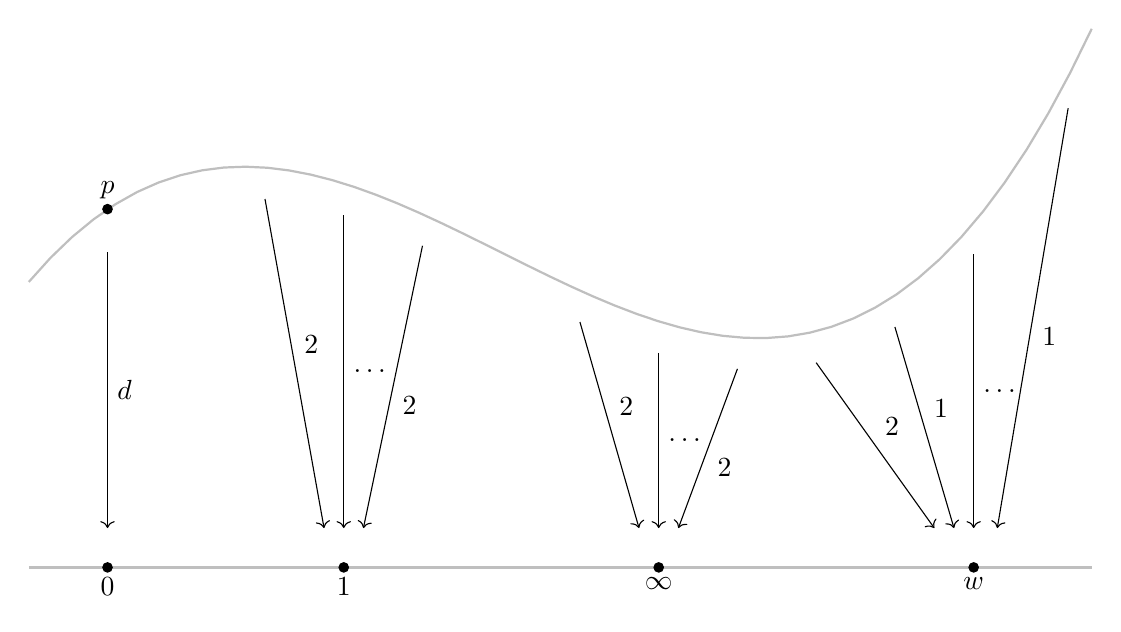
\begin{tikzpicture}
  \draw[domain=-6:7.5,samples=50,color=gray!50,thick] plot (\x, \x^3/64 - \x/2); % Curve E
  \draw[domain=-6:7.5,samples=50,color=gray!50,thick] plot (\x, -4); % P^1

  \filldraw[black] (-5, .55) circle (0.6mm) node[above] {$p$};

  % fiber over 0
  \draw[->] (-5, 0) to["$d$"] (-5, -3.5);

  % fiber over 1
  \foreach \x/\l in {-3/$2$, -2/$\dots$, -1/$2$} {
    \draw[->] (\x, \x^3/64-\x/2-.4) to["\l"] (-3/2+\x/4, -3.5);
  }

    % fiber over infinity
  \foreach \x/\l in {1/$2$, 2/$\dots$, 3/$2$} {
    \draw[->] (\x, \x^3/64-\x/2-.4) to["\l"] (3/2+\x/4, -3.5);
  }

  % fiber over w
  \foreach \x/\l in {4/$2$, 5/$1$, 6/$\dots$, 7.2/$1$} {
    \draw[->] (\x, \x^3/64-\x/2-.4) to["\l"] (9/2+\x/4, -3.5);
  }

  % 0, 1, infinity, w
  \foreach \x/\l in {-5/$0$, -2/$1$, 2/$\infty$, 6/$w$} {
    \filldraw[black] (\x, -4) circle (0.6mm) node[below] {\l};
    }

\end{tikzpicture}

\label{fig:twos}
\end{figure}

  The latter count is given by
  \[
  H((d),(2^k),(2^k),(2,1,\dots,1))
  \]
  which is $k/2$ by Claim~\ref{claim:twoscomplete}. For the former count, we
  first consider maps $\P^1\to\P^1$  (with $0,1,\infty,w$ fixed)
  described in Figure \ref{fig:comb1} or \ref{fig:comb2}, depending on the parity of $k$:

  \begin{itemize}
  \item If $k$ is odd, the orbifold number of such maps is $H((k),(2^{(k-1)/2},1),(2^{(k-1)/2},1))$ which
    equals $1$ by Claim~\ref{claim:twosodd}. There are $k$ choices for $q_1,q_2,q_3,q_4$
    since $q_2$ and $q_3$ are determined and there are $k$ choices for $q_4$.
  \item If $k$ is even, the orbifold number of such maps is $H((k),(2^{k/2-1},1,1),(2^{k/2}))$ which equals $\frac 12$ by Claim~\ref{claim:twoseven}. There are $2k$ choices for $q_1,q_2,q_3,q_4$
    since there are two choices for labeling $q_2$ and $q_3$, and there are $k$ choices for
    $q_4$.
  \end{itemize}
  In either case, the orbifold number of such covers with $q_1,q_2,q_3,q_4$ labeled is $k$.

  Once $q_1,q_2,q_3,q_4$ are fixed, the count for the upstairs map $E\to\P^1$ is
  $H((2),(2),(2),(2))=\frac 12$. Thus, the orbifold number of factored maps lying over $0,1,\infty,w$ is $\frac 12\cdot k$, proving the claim.
  
\end{proof}

Now given this result, we can compute $N_{(2^k),(2^k)}(d)$ by counting
the number of factored maps described in Figures \ref{fig:comb1} and \ref{fig:comb2} for a fixed $(E,p)$.
The map $(E,p)\to(\P^1,q_1)$ is the elliptic map to $\P^1$ and therefore unique up
to automorphisms of $\P^1$.
There are $3$ choices for the point
$q_4$, and we consider each parity case:
\begin{itemize}
\item If $k$ is odd, then the orbifold count of maps
  $\P^1\to\P^1$ with ramification profiles $(k)$ over $0$,
  $(2^{(k-1)/2},1)$ over $1$, and $(2^{(k-1)/2},1)$ over $\infty$
  is $1$. There is a unique way to assign $q_2$ lying over $1$
  and $q_3$ lying over $\infty$.
  \item
  If $k$ is even, then the orbifold count of maps $\P^1\to\P^1$ with
  ramification profiles $(k)$ over $0$, $(2^{k/2-1},1,1)$ over $1$, and
  $(2^{k/2})$ over $\infty$ is $\frac 12$. There are two choices for
  labeling $q_2$ and $q_3$, so with $q_1,q_2,q_3$ fixed, the number
  of covers is $\frac 12\cdot 2=1$.
\end{itemize}
In either case, $w$ is determined as the image of $q_4$.
Therefore,
\[
N_{(2^k),(2^k)}(d)=3.
\]

\subsection{Genus reduction}

We apply the method of Section 3 to yield another proof that
$N_{(2^k),(2^k)}(d)=3$:

 Let $A$ be a stable graph consisting of a genus $0$ vertex with a loop and a marked point $p_{1,1}$.
  Let $\hat A$ be the stable graph with additional marked points on the genus $0$ vertex for
  the further ramification.

There are two kinds of
admissible covers $\Gamma\to\Gamma'$ with $\Gamma$ specializing to $\hat A$. The first
is of the form:

\begin{figure}[h]
  \caption{First admissible cover $\Gamma\to\Gamma'$ in ``all twos'' genus reduction}
\begin{tikzpicture}[thick]

  \matrix[amat,nodes=fsnode] (mat1) {$0$\\};

    \matrix[dmat,left=1cm of mat1] (degrees1) {$d$\\};


 \matrix[amat,right=4cm of mat1,nodes=ssnode] (mat2) {$0$\\};

 \matrix[dmat,right=1cm of mat2] (degrees2) {$d$\\};

 \draw  (mat1-1-1) edge["$a$",bend left] (mat2-1-1)
 (mat1-1-1) edge["$b$"] (mat2-1-1);

  % draw legs for left side
 \draw (mat1-1-1) -- +(95:.58) node[anchor=south] {$p_{1,1}$}
 (mat1-1-1) -- +(245:.58) node[anchor=north] {$(2,1^{d-2})$};

 % draw legs for right side
 \draw  (mat2-1-1) -- +(30:.58) node[anchor=west] {$(2^k)$}
 (mat2-1-1) -- +(330:.58) node[anchor=west] {$(2^k)$};

\end{tikzpicture}
\end{figure}

            There are two $\hat A$-structures, corresponding to a choice
            of edge to contract, and so $c_{\Gamma}=a+b=d$. The right-hand count here under Theorem~\ref{thm:admissible} is
            \begin{align*}
              \overline H((d),(a,b),(2,1^{d-2}))\cdot \overline H((2^k),(2^k),(a,b))\cdot d\cdot\frac 1{|\Aut(a,b)|}
            \end{align*}
            By Claim~\ref{claim:twoscycles} in Appendix~\ref{appendix:hurwitz}, the second term vanishes unless $a=b=k$, in which case
            the count (by Claims~\ref{claim:twoscycles} and \ref{claim:Hurwitz2}) is
            \[
            (1\cdot (d-2)!)\cdot \left(\frac 1d\cdot k!\cdot k!\cdot 2\right)\cdot d\cdot\frac 12
            =(d-2)!\cdot (k!)^2
            \]

            Now the second picture is of the form shown in Figure~\ref{fig:secondalltwos}.
            With markings remembered, the number of such diagrams is
            \[
            2\cdot k\cdot\binom{d-2}{2}\cdot\binom{d-4}{2}\cdot\dots\cdot\binom 22=2k\cdot\frac{(d-2)!}{2^{k-1}}
            \]
                        \begin{figure}[h]
              \caption{Second admissible cover $\Gamma\to\Gamma'$ in ``all twos'' genus reduction}
              \centering
            \begin{tikzpicture}[thick]

  \matrix[amat,nodes=fsnode] (mat1) {$0$\\};

    \matrix[dmat,left=1cm of mat1] (degrees1) {$d$\\};


 \matrix[amat,right=4cm of mat1,nodes=ssnode] (mat2) {$0$\\
      $0$\\
      $\vdots$\\
  $0$\\};

 \matrix[dmat,right=1cm of mat2] (degrees2) {$2$\\
   $2$ \\
    \vdots \\
    $2$\\};

 \draw  (mat1-1-1) edge["$1$",bend left] (mat2-1-1)
 (mat1-1-1) edge["$1$"] (mat2-1-1)
 (mat1-1-1) edge["$2$"] (mat2-2-1)
 (mat1-1-1) edge["$2$"] (mat2-4-1);

  % draw legs for left side
 \draw (mat1-1-1) -- +(95:.58) node[anchor=south] {$p_{1,1}$}
 (mat1-1-1) -- +(245:.58) node[anchor=north] {$(2^k)$};

 % draw legs for right side
 \draw  (mat2-1-1) -- +(30:.58) node[anchor=west] {$2$}
 (mat2-1-1) -- +(330:.58) node[anchor=west] {$2$}
 (mat2-2-1) -- +(330:.58) node[anchor=west] {$2$}
 (mat2-4-1) -- +(330:.58) node[anchor=west] {$2$};

            \end{tikzpicture}
            \label{fig:secondalltwos}
            \end{figure}
            There are two $\hat A$-structures, each with associated coefficient $2^{k-1}$,
            and so the combined contribution to the right-hand side of Theorem~\ref{thm:admissible} is
            \begin{align*}
              &2k\cdot\frac{(d-2)!}{2^{k-1}}\cdot\overline H((d),(2^k),(2^{k-1},1,1))\cdot \overline H((1,1),(2),(2))\cdot \overline H((2),(2),(1,1))^{k-1}\cdot\frac 12\cdot 2\cdot 2^{k-1} \\
              &=2k\cdot (d-2)!\cdot (k!\cdot (k-1)!) \\
              &=2(d-2)!\cdot (k!)^2
            \end{align*}
            We conclude by adding up and seeing that the right-hand side of Theorem~\ref{thm:admissible} is
            \begin{align*}
              (d-2)!\cdot (k!)^2+ 2(d-2)!\cdot (k!)^2=3(d-2)!\cdot (k!)^2&\implies W_{(2^k),(2^k),(2,1^{d-2})}(d)=6(d-2)!\cdot (k!)^2 \\
              &\implies N_{(2^k),(2^k)}(d)=3.
            \end{align*}


\section{Recursion and general solution}

We now aim to find a recursion for the terms $N_{(2^k),(2^k)}(\mu)$. In particular we will show:

\begin{thm}
  If $a>b$, $\mu=(a,b,\mu')$ and $d'=|\mu'|$, then
  \[
  N_{(2^k),(2^k)}(a,b,\mu')=N_{(2^k),(2^k)}(a+b,\mu')+n_{a,b,d'}N_{(2^{k-b}),(2^{k-b})}(a-b,\mu')
  \]
  where \[n_{a,b,d'}=\begin{cases}
  3 & a-b=2,\ d'=0 \\
  6 & a-b=1,\ d'=1 \\
  1 & d-2b>2 \end{cases}
  \]
  and
  \[
  N_{(2^k),(2^k)}(a,a,\mu')=
  N_{(2^k),(2^k)}(2a,\mu')+
  \begin{cases}
    2N_{(2^{k-a}),(2^{k-a})}(\mu') & |\mu'|>2 \\
    3 & |\mu'|=0 \\
    6 & \mu'=(2) \\
    12 & \mu'=(1,1)
    \end{cases}
  \]
  \end{thm}
\begin{proof}
  We will use Theorem~\ref{thm:admissible} to compute $W_{(2^k),(2^k),(2,1^{d-2})^{\ell(\mu)}}(a,b,\mu')$,
  letting $A$ be the graph with a genus $1$ vertex containing
  $p_{1,3},\dots,p_{1,\ell(\mu)}$ connected to a genus $0$ vertex containing $p_{1,1}$ and $p_{1,2}$.
  Any admissible cover of graphs $\Gamma\to\Gamma'$ has precisely two branch points that do
  not arise from the genus $1$ vertex of $\Gamma$, by Lemma~\ref{lem:branchpoints}.

  Suppose the points $p_{1,1},\dots,p_{1,\ell(\mu)}$ appear on the right side of $\Gamma$, i.e.
  their images are not on the same component as the image of the genus $1$ vertex. If
  $p_{1,1}$ and $p_{1,2}$ are on the same component, then we have the picture shown in Figure~\ref{fig:alltwos1}.

  \begin{figure}[h]
    \caption{First cover $\Gamma\to\Gamma'$ in ``all twos'' recursion}
    \centering
  \begin{tikzpicture}[thick]

  \matrix[amat,nodes=fsnode] (mat1) {$1$\\
    $0$\\
    \vdots \\
  $0$\\};

  \matrix[dmat,left=2cm of mat1] (degrees1) {$d-\sum c_i$\\
    $c_1$\\
    \vdots \\
  $c_r$\\};

 \matrix[amat,right=7cm of mat1,nodes=ssnode] (mat2) {$0$\\
   \vdots\\
   $0$ \\
   $0$\\};
 \matrix[dmat,right=1.5cm of mat2] (degrees2) {$\mu_{\ell(\mu)}$\\
   \vdots\\
   $\mu_3$ \\
 $a+b$\\};

 \draw  (mat1-1-1) edge["$\mu_{\ell(\mu)}$"] (mat2-1-1)
 (mat1-1-1) edge["$\mu_{3}$"] (mat2-3-1)
 (mat1-1-1) edge["$a+b-\sum c_i$"] (mat2-4-1)
 (mat1-2-1) edge["$c_1$"] (mat2-4-1)
 (mat1-4-1) edge["$c_r$"] (mat2-4-1);


 % draw legs for right side
 \draw  (mat2-1-1) -- +(30:.58) node[anchor=west] {$p_{1,\ell(\mu)}$}
 (mat2-3-1) -- +(30:.58) node[anchor=west] {$p_{1,3}$}
 (mat2-4-1) -- +(30:.58) node[anchor=west] {$p_{1,2}$}
 (mat2-4-1) -- +(330:.58) node[anchor=west] {$p_{1,1}$};

  \end{tikzpicture}
  \label{fig:alltwos1}
  \end{figure}

  Riemann-Hurwitz for the bottom-right vertex tells us that there must be
  \[
  2(a+b)-2-(a+b-2)-\left(a+b-\sum c_i-1+\sum(c_i-1)\right)=1+r
  \]
  additional ramification on that vertex.
  If $\ell(\mu')=0$ and there is a ramification profile of $(2^k)$ on the right side,
  then $1+r=k$ and $r=k-1$ with $a+b=2k$. Since there must be a ramification
  profile $(2^k)$ on the left, we have $c_i=2$ for all $i$ and the simplified picture in Figure~\ref{fig:alltwos1simplified}.

  \begin{figure}[h]
    \caption{Simplification of Figure~\ref{fig:alltwos1}}
    \centering
    \begin{tikzpicture}[thick]

  \matrix[amat,nodes=fsnode] (mat1) {$1$\\
    $0$\\
    \vdots \\
  $0$\\};

  \matrix[dmat,left=2cm of mat1] (degrees1) {$2$\\
    $2$\\
    \vdots \\
  $2$\\};

  \matrix[amat,right=7cm of mat1,nodes=ssnode] (mat2) {$0$\\};
  
 \matrix[dmat,right=1.5cm of mat2] (degrees2) {$d$\\};

 \draw  (mat1-1-1) edge["$2$"] (mat2-1-1)
 (mat1-2-1) edge["$2$"] (mat2-1-1)
 (mat1-4-1) edge["$2$"] (mat2-1-1);

  % draw legs for left side
 \draw  (mat1-1-1) -- +(50:.58) node[anchor=south] {$2$}
 (mat1-1-1) -- +(110:.58) node[anchor=south] {$2$}
 (mat1-1-1) -- +(170:.58) node[anchor=east] {$2$}
 (mat1-2-1) -- +(50:.58) node[anchor=south] {$2$}
 (mat1-4-1) -- +(50:.58) node[anchor=south] {$2$};

 % draw legs for right side
 \draw  (mat2-1-1) -- +(50:.58) node[anchor=south] {$p_{1,1}$}
 (mat2-1-1) -- +(115:.58) node[anchor=south] {$p_{1,2}$}
 (mat2-1-1) -- +(260:.58) node[anchor=north] {$(2^k)$};

    \end{tikzpicture}
    \label{fig:alltwos1simplified}
    \end{figure}

    By Claim~\ref{claim:twoscycles}, the Hurwitz number $H((2^k),(2^k),(a,b))$ on the right
    side vanishes unless $a=b$.
    If $a=b$, then the contribution of this picture to $W_{(2^k),(2^k),(2,1^{d-2})^{\ell(\mu)}}(a,a)$ is
    \begin{align*}
      &2\cdot k\cdot \binom{d-2}{2,\dots,2}^2\cdot W_{(2),(2),(2)}(2)\cdot \overline H((2),(2),(1,1),(1,1))^{k-1}\cdot \overline H((2^k),(2^k),(k,k))\cdot 2^{k-1} \\
      &=2k\cdot\frac{((d-2)!)^2}{2^{2k-2}}\cdot 6\cdot 2^{k-1}\cdot (k!)^2\cdot\frac 1k\cdot 2^{k-1} \\
      &=2\cdot 6\cdot ((d-2)!)^2\cdot\frac{2^{2k-2}}{2^{2k-2}}\cdot (k!)^2 \\
      &=12((d-2)!)^2\cdot (k!)^2
      \end{align*} %TODO: make lines shorter
    so the contribution to $N_{(2^k),(2^k)}(a,a)$ is
    $\frac{12((d-2)!)^2(k!)^2}{(k!)^2\cdot 2\cdot ((d-2)!)^2\cdot 2!}=3$ (corresponding to a choice of nontrivial 2-torsion point).
  
  Otherwise if $\ell(\mu')>0$ there cannot be a ramification profile of $(2^k)$
  on the right side, the additional ramification must be simple, and so $r=0$.
  Upon
  choosing which fiber of simple branching will appear on the right side and how it will appear,
  for which there are
  \[
  C=\ell(\mu)\cdot \binom{d-2}{a+b-2,\mu_3,\dots,\mu_{\ell(\mu)}}
  \]
  %TODO: say some version of Theorem 3.1 which uses N, A and not W, hat(A)?
  choices, there is a unique such map $\Gamma\to\Gamma'$, and $\Gamma$ has a unique $\hat A$-structure
  with $c_{\Gamma}=\prod\limits_{i=3}^{\ell(\mu)}\mu_i$, so the corresponding contribution to the right side of Theorem~\ref{thm:admissible} in this case is
  \begin{align*}
    &C\cdot W_{(2^k),(2^k),(2,1^{d-2})^{\ell(\mu)-1}}(a+b,\mu') \prod_{i=3}^{\ell(\mu)}\overline H((\mu_i),(\mu_i),(1^{\mu_i})) \cdot \overline H((a+b),(a,b),(2,1^{a+b-2})) c_{\Gamma} \\
    &=\frac{\ell(\mu)(d-2)!\cdot (k!)^2\cdot 2\cdot ((d-2)!)^{\ell(\mu)-1}(\ell(\mu)-1)!}{(a+b-2)!\mu_3!\cdots\mu_{\ell(\mu)}!}\cdot N_{(2^k),(2^k)}(a+b,\mu')\cdot \prod_{i=3}^{\ell(\mu)}\mu_i!\cdot (a+b-2)! \tag*{(using Claim~\ref{claim:Hurwitz2})} \\
    &=(\ell(\mu))!\cdot (k!)^2\cdot 2\cdot((d-2)!)^{\ell(\mu)}\cdot N_{(2^k),(2^k)}(a+b,\mu') \\
  \end{align*}

  and the left side is the $W$ invariant of interest, since $A$ has no nontrivial automorphisms. Thus,
  the contribution to $N_{(2^k),(2^k)}(a,b,\mu')$ is
  \begin{align*}
    \frac{(\ell(\mu))!\cdot (k!)^2\cdot 2\cdot((d-2)!)^{\ell(\mu)}\cdot N_{(2^k),(2^k)}(a+b,\mu')}{(k!)^2\cdot 2\cdot((d-2)!)^{\ell(\mu)}\cdot (\ell(\mu))!} =N_{(2^k),(2^k)}(a+b,\mu').
  \end{align*}

  Next, consider the case where $p_{1,1}$ and $p_{1,2}$ are not on the same component, in which
  case at least one vertex containing one of these two contains some additional ramification
  (necessarily simple).
  This then exhausts the branch points not arising from the genus $1$ vertex, so we have the picture
  in Figure~\ref{fig:alltwoscase2}.


    \begin{figure}[h]
    \caption{Second cover $\Gamma\to\Gamma'$ in ``all twos'' recursion}
    \centering
    \begin{tikzpicture}[thick]

  \matrix[amat,nodes=fsnode] (mat1) {$1$\\
    $0$\\};

  \matrix[dmat,left=2cm of mat1] (degrees1) {$d-2e$\\
    $2e$\\};

 \matrix[amat,right=7cm of mat1,nodes=ssnode] (mat2) {$0$\\
   $0$ \\
   $0$ \\
   $0$\\
 $0$\\};
 \matrix[dmat,right=1.5cm of mat2] (degrees2) {$\mu_{\ell(\mu)}$\\
   \vdots\\
   $\mu_3$ \\
   $a$\\
 $b$\\};

 \draw  (mat1-1-1) edge["$\mu_{\ell(\mu)}$"] (mat2-1-1)
 (mat1-1-1) edge["$\mu_{3}$"] (mat2-3-1)
 (mat1-1-1) edge["$a+b-2e$"] (mat2-4-1)
 (mat1-2-1) edge["$2e-b$"] (mat2-4-1)
 (mat1-2-1) edge["$b$"] (mat2-5-1);


 % draw legs for right side
 \draw  (mat2-1-1) -- +(30:.58) node[anchor=west] {$p_{1,\ell(\mu)}$}
 (mat2-3-1) -- +(30:.58) node[anchor=west] {$p_{1,3}$}
 (mat2-4-1) -- +(30:.58) node[anchor=west] {$p_{1,1}$}
 (mat2-4-1) -- +(310:.58) node[anchor=west] {$(2,1^{a-2})$}
 (mat2-5-1) -- +(30:.58) node[anchor=west] {$p_{1,2}$};

  % draw legs for left side
 \draw  (mat1-2-1) -- +(30:.58) node[anchor=west] {$(2^e)$}
 (mat1-2-1) -- +(80:.58) node[anchor=south] {$(2^e)$};

    \end{tikzpicture}
    \label{fig:alltwoscase2}
    \end{figure}

    By Claim~\ref{claim:twoscycles}, $\overline H((2^e),(2^e),(2e-b,b))$ vanishes
    unless $b=e$ (which requires $a+b-2e=a-b>0\iff a>b$).
    Let $n_{a,b,d'}$ be the number of choices for the fibers in which to place
    the even ramification on the bottom left vertex. If $d-2b=a-b+d'$ (where
    $d'=|\mu'|$) is equal to $2$, then either $a-b=2$, $d'=0$, and $n_{a,b,d'}=\binom 32=3$
    since there are three ramified points on the genus $1$ vertex,
    or $a-b=d'=1$ and $n_{a,b,d'}=\binom 42=6$ since there are four ramified points on
    the genus $1$ vertex. If $d-2b>2$, then there are only two evenly ramified
    fibers on the genus $1$ vertex, so the placement of even ramification
    on the bottom left vertex is determined and $n_{a,b,d'}=1$.
    
    In any case the corresponding
    contribution to $W_{(2^k),(2^k),(2,1^{d-2})^{\ell(\mu)}}(a,b,\mu')$ is

    \begin{align*}
      &n_{a,b,d'}\ell(\mu)\binom{d-2}{a-2,b,\mu_3,\dots,\mu_{\ell(\mu)}}\binom{k}{b}^2\binom{d-2}{2b}^{\ell(\mu)-1}W_{(2^{k-b}),(2^{k-b}),(2,1^{d-2b-2})^{\ell(\mu)-1}}(a-b,\mu') \cdot \\
      &\overline H((2^b),(2^b),(b,b),(1^{2b})^{\ell(\mu)-1}) \cdot\prod_{i=3}^{\ell(\mu)}
      \overline H((\mu_i),(\mu_i),(1^{\mu_i}))\mu_i\cdot \overline H((a-b,b),(a),(2,1^{a-2}))\overline H((b),(b),(1^b))b^2 \\
      &=n_{a,b,d'}\ell(\mu)\frac{(d-2)!(k!)^2((d-2)!)^{\ell(\mu)-1}}{(a-2)!b!\mu_3!\cdots\mu_{\ell(\mu)}!(b!)^2((k-b)!)^2((2b)!(d-2b-2)!)^{\ell(\mu)-1}}N_{(2^{k-b}),(2^{k-b})}(a-b,\mu')\cdot \\
      &2((k-b)!)^2\cdot ((d-2b-2)!)^{\ell(\mu)-1}(\ell(\mu)-1)! \cdot\frac 1{2b}(b!)^2\cdot 2\cdot ((2b)!)^{\ell(\mu)-1}\cdot \mu_3!\cdots\mu_{\ell(\mu)}!(a-2)!b!\cdot b \\
      &=n_{a,b,d'}(\ell (\mu))!N_{(2^{k-b}),(2^{k-b})}(a-b,\mu')\cdot (k!)^2\cdot 2\cdot ((d-2)!)^{\ell(\mu)}
    \end{align*}
    so the contribution to $N_{(2^k),(2^k),(2,1^{d-2})^{\ell(\mu)}}(a,b,\mu')$ is $n_{a,b,d'}N_{(2^{k-b}),(2^{k-b})}(a-b,\mu')$.

    We can now turn to the situation where $p_{1,1},\dots,p_{1,\ell(\mu)}$ appear
    on the left side of $\Gamma$, i.e.\ where their images are on the same
    component as the image of the genus $1$ vertex. Since $p_{1,1}$ is not on the
    genus $1$ vertex, its path to the genus $1$ vertex must pass through
    a vertex on the right side, yielding at least two branch points.
    If any of $p_{1,3},\dots,p_{1,\ell(\mu)}$ were not on the genus $1$ vertex then
    this would be true of another vertex, implying that both fibers of
    ramification profile $(2^k)$ are on the right side and there is only
    simple ramification on the genus $1$ vertex (contradicting
    dimensional assumptions).

    If $p_{1,1}$ and $p_{1,2}$ are on different components, we have the picture in Figure~\ref{fig:impossiblecover}.
    This is impossible by Riemann-Hurwitz for the bottom-right vertex, and so
    we are left with one remaining picture to consider where $p_{1,1}$ and
    $p_{1,2}$ appear on the same component (here $2e=a+b$), in Figure~\ref{fig:thirdcoveralltwos}.



      \begin{figure}[h]
    \caption{Impossible cover $\Gamma\to\Gamma'$ in ``all twos'' recursion}
    \centering
        \begin{tikzpicture}[thick]

  \matrix[amat,nodes=fsnode] (mat1) {$1$\\
    $0$\\
  $0$\\};

  \matrix[dmat,left=0.6cm of mat1] (degrees1) {$d-a-b$\\
    $a$\\
  $b$\\};

 \matrix[amat,right=6cm of mat1,nodes=ssnode] (mat2) {$0$\\
   $0$ \\
   $0$ \\
   $0$\\};
 \matrix[dmat,right=1.7cm of mat2] (degrees2) {$1$\\
   \vdots\\
   $1$ \\
   $e$\\};

 \draw  (mat1-1-1) edge["$1$"] (mat2-1-1)
 (mat1-1-1) edge["$1$"] (mat2-3-1)
 (mat1-1-1) edge["$e-a-b$"] (mat2-4-1)
 (mat1-2-1) edge["$a$"] (mat2-4-1)
 (mat1-3-1) edge["$b$"] (mat2-4-1);


 % draw legs for right side
 \draw  
 (mat2-4-1) -- +(30:.58) node[anchor=west] {$(2,1^{e-2})$}
 (mat2-4-1) -- +(310:.58) node[anchor=west] {$(2,1^{e-2})$};

  % draw legs for left side
 \draw  (mat1-2-1) -- +(30:.58) node[anchor=west] {$p_{1,1}$}
 (mat1-3-1) -- +(30:.58) node[anchor=west] {$p_{1,2}$};

        \end{tikzpicture}
        \label{fig:impossiblecover}
        \end{figure}

          \begin{figure}[h]
    \caption{Third cover $\Gamma\to\Gamma'$ in ``all twos'' recursion}
    \centering
                \begin{tikzpicture}[thick]

  \matrix[amat,nodes=fsnode] (mat1) {$1$\\
    $0$\\};

  \matrix[dmat,left=2cm of mat1] (degrees1) {$d-2e$\\
    $2e$\\};

 \matrix[amat,right=7cm of mat1,nodes=ssnode] (mat2) {$0$\\
   $0$ \\
   $0$ \\
   $0$\\
   $0$\\
   $0$\\
 $0$\\};
 \matrix[dmat,right=1.5cm of mat2] (degrees2) {$1$\\
   \vdots\\
   $1$ \\
   $2$\\
   $1$\\
   \vdots\\
 $1$\\};

 \draw  (mat1-1-1) edge["$1$"] (mat2-1-1)
 (mat1-1-1) edge["$1$"] (mat2-3-1)
 (mat1-1-1) edge["$1$"] (mat2-4-1)
 (mat1-2-1) edge["$1$"] (mat2-4-1)
 (mat1-2-1) edge["$1$"] (mat2-5-1)
 (mat1-2-1) edge["$1$"] (mat2-7-1);


 % draw legs for right side
 \draw  
 (mat2-4-1) -- +(30:.58) node[anchor=west] {$2$}
 (mat2-4-1) -- +(310:.58) node[anchor=west] {$2$};

  % draw legs for left side
 \draw  (mat1-2-1) -- +(50:.58) node[anchor=west] {$p_{1,1}$}
 (mat1-2-1) -- +(80:.58) node[anchor=south] {$p_{1,2}$}
 (mat1-2-1) -- +(160:.58) node[anchor=east] {$(2^e)$}
 (mat1-2-1) -- +(220:.58) node[anchor=north] {$(2^e)$};

                \end{tikzpicture}
                \label{fig:thirdcoveralltwos}
                \end{figure}

                By Claim~\ref{claim:twoscycles}, $\overline H((a,b),(2^e),(2^e))$ vanishes unless $a=b$.
                There are $\binom{\ell(\mu)}{2}$ choices for simple ramification profiles to place on the right
                side, $\binom{d-2}{2a-1}$ choices for which unramified points appear in the top right
                and bottom right corners of the diagram within the first chosen simple ramification profile,
                $(d-2)!$ choices for placement of unramified points in the second chosen
                right simple ramification profile, $\binom ka^2$ choices for placement of even ramification profiles
                on the left side, and $\binom{d-2}{2a}^{\ell(\mu)-2}$ choices for placement of unramified points in
                simple ramification profiles on the left side.
                As for choices of placement for even ramification:
                \begin{itemize}
                  \item
                If $\mu'=(2)$, then there are $3$ unmarked ramified points on
                the genus $1$ vertex, and two must be marked as being in
                even ramification fibers, yielding $\binom 32=3$ choices.
              \item If $\mu'=(1,1)$, then there are
                $4$ unmarked ramified points on the genus $1$ vertex,
                yielding $\binom 42=6$ choices.
              \item If $d'>2$, then there is a single choice, as the
                genus $1$ vertex unambiguously has two even ramification profiles.
                \end{itemize}
                

                
                We also have $c_{\Gamma}=2$, since there are two ways to contract
                edges of the graph to obtain a stabilization (one, but not
                both, of the edges from the degree $2$ vertex on the right
                will be contracted).
                There are also $d-2a-1$ unfixed points to be ordered
                on the genus $1$ vertex
                corresponding to all but one of its edges.
                Therefore the total
                contribution to $W_{(2^k),(2^k),(2,1^{d-2})^{\ell(\mu)}}(a,a,\mu')$ in this case is
                \begin{align*}
                  &\binom{\ell(\mu)}{2}\frac{((d-2)!)^2}{(2a-1)!(d-2a-1)!}\binom ka^2\binom{d-2}{2a}^{\ell(\mu)-2}W_{(2^{k-a}),(2^{k-a}),(2,1^{d-2a-2})^{\ell(\mu)-2}}(\mu')\cdot (d-2a-1)!\cdot  \\
                  &
                  \overline H((a,a),(2^a),(2^a),(1^{2a})^{\ell(\mu)-1}) \cdot
                  \overline H((2),(2),(1,1))\cdot 2 \\
                  &=\frac{(\ell(\mu))(\ell(\mu)-1)((d-2)!)^2}{2(2a-1)!}\frac{(k!)^2}{(a!(k-a)!)^2}\frac{((d-2)!)^{\ell(\mu)-2}}{((2a)!(d-2a-2)!)^{\ell(\mu)-2}}((k-a)!)^2\cdot 2 \cdot \\
                  &((d-2a-2)!)^{\ell(\mu)-2}\cdot (\ell(\mu)-2)!N_{(2^{k-a}),(2^{k-a})}(\mu')\cdot\frac{((2a)!)^{\ell(\mu)-1}((a!)^2)}{a}\cdot 2 \\
                  &=\frac{2(\ell(\mu))!((d-2)!)^{\ell(\mu)}(k!)^2N_{(2^{k-a}),(2^{k-a})}(\mu')
                  (2a)!}{(2a-1)!a} \\
                  &=2N_{(2^{k-a}),(2^{k-a})}(\mu')\cdot (k!)^2\cdot 2\cdot ((d-2)!)^{\ell(\mu)}\cdot (\ell(\mu))!
                \end{align*}
                multiplied by $3$ if $\mu'=(2)$ or by $6$ if $\mu'=(1,1)$.
                Therefore the corresponding contribution
                to $W_{(2^k),(2^k)}(a,a,\mu')$ is $2N_{(2^{k-a}),(2^{k-a})}(\mu')$
                if $d'>2$, $3\cdot 2\cdot 1=6$ if $\mu'=(2)$, and
                $6\cdot 2\cdot 1=12$ if $\mu'=(1,1)$.

\end{proof}

\begin{cor}
  \label{cor:twos}
  Let $d=2k$ be any even integer greater than $2$. For any $\mu$ with sum $|\mu|=d$, $N_{(2^k),(2^k)}(\mu)=3\cdot 2^{\ell(\mu)-1}$.
\end{cor}
\begin{proof}
  We can prove this by induction on $\ell(\mu)$; the base case $\ell(\mu)=1$ was proven in Theorem~\ref{thm:combinatorial}. Assume
  the result for all $\nu$ with $\ell(\nu)< r$, and suppose $\ell(\mu)=r\geq 2$.
  Then we can write $\mu=(a,b,\mu')$ with $d'=|\mu'|$. If $a=b$, then we have
  four cases:
  \begin{enumerate}
  \item If $\mu'$ is empty: $N_{(2^k),(2^k)}(a,a)=N_{(2^k),(2^k)}(2a)+3=3+3=3\cdot 2^{r-1}$
  \item If $\mu'=(2)$: $N_{(2^k),(2^k)}(a,a,2)=N_{(2^k),(2^k)}(2a,2)+6=6+6=12=3\cdot 2^{r-1}$
  \item If $\mu'=(1,1)$: $N_{(2^k),(2^k)}(a,a,1,1)=N_{(2^k),(2^k)}(2a,1,1)+12=12+12=3\cdot 2^{r-1}$
  \item If $d'>2$:
      \begin{align*}
    N_{(2^k),(2^k)}(a,a,\mu') &= N_{(2^k),(2^k)}(2a,\mu')+2N_{(2^{k-a}),(2^{k-a})}(\mu') \\
    &=3\cdot 2^{r-2}+2(3\cdot 2^{r-3}) \\
    &=3\cdot 2^{r-1}
  \end{align*}

    \end{enumerate}
  Now if $a>b$ (without loss of generality), we have three cases:
  \begin{enumerate}
  \item If $a-b=2$ and $d'=0$:
    \[
    N_{(2^k),(2^k)}(a,a-2)=N_{(2^k),(2^k)}(2a-2)+3N_{(2),(2)}(2)=3+3\cdot 1=6=3\cdot 2^{r-1}
    \]
  \item If $a-b=1$ and $d'=1$:
    \[
    N_{(2^k),(2^k)}(a,a-1,1)=N_{(2^k),(2^k)}(2a-1,1)+6N_{(2),(2)}(1,1)=6+6\cdot 1=12=3\cdot 2^{r-1}
    \]
    \item If $d-2b>2$:
    \begin{align*}
      N_{(2^k),(2^k)}(a,b,\mu') &= N_{(2^k),(2^k)}(a+b,\mu')+2N_{(2^{k-b}),(2^{k-b})}(a-b,\mu') \\
      &= 3\cdot 2^{r-2}+3\cdot 2^{r-2} \\
      &= 3\cdot 2^{r-1}.
    \end{align*}
    \end{enumerate}
  \end{proof}

\chapter{Invariants $S_{\a,\b}$}

In this chapter, we consider a family of invariants $N_{g,\sigma,\nu}$ where
one ramification profile
$\mu$ is fully marked,
each other ramification profile $\sigma_i$ is of the form $(a,1,\dots,1)$, and
the only ``remembered'' points in these ramified fibers are some subset of the ones with
a nontrivial ramification index. We will establish general recursive formulas
(Theorems~\ref{thm:reduceb} and \ref{thm:reducea})
that allow us to compute this family of invariants, and will establish
specific closed-forms in special cases.


\section{Definitions and basic results}

Fix a degree $d\geq 1$. For any partition $\mu$ of $d$, and multisets $\a$ and $\b$ of
positive integers less than or equal to $d$, let
\[
S_{\a,\b}(\mu)=N_{1,\sigma,\nu}
\]
where
\[
\sigma=\{\mu\}\cup\{(x,1,\dots,1):x\in\a\cup\b\},\quad \nu=\{\mu\}\cup\{(x,1,\dots,1):x\in\b\}
\]
By Riemann-Hurwitz,
\[
d-\ell(\mu)+\sum_{x\in\a\cup\b}(x-1)=2d.
\]
We will use the convention that $x_1,\dots,x_{\ell(\mu)}$
form the fiber corresponding to $\mu$, $p_{i,1},\dots,p_{i,d-a_i+1}$ form
the fiber corresponding to the $i^{\text{th}}$ value $a_i\in\a$, and
$P_{i,1},\dots,P_{i,d-b_i+1}$ form the fiber corresponding to the
$i^{\text{th}}$ value $b_i\in\b$.

\begin{prop}
  Elements $1$ in $\b$ can be removed:
  $S_{\a,\b+\{1\}}(\mu)=S_{\a,\b}(\mu)$.
  We can therefore assume without loss of generality that $\b$ contains integers greater than $1$.
\end{prop}
\begin{proof}
  The addition of a ramification profile $(1,\dots,1)$ does not affect
  our counting problem, since this is the generic form of a fiber;
  imposing that one marked point on the
  generic genus $1$
  marked curve is part of a generic fiber is no restriction at all.

  More formally,
  we have the following commutative diagram:

  \[\begin{tikzcd}
\Hb_{1,\sigma+\{(1,\dots,1)\}} & \overline{\mathcal M}_{1,\ell(\b)+1} \\
\Hb_{1,\sigma} & \overline{\mathcal M}_{1,\ell(\b)}
	\arrow[from=1-1, to=1-2, "\pi'"]
	\arrow[from=1-1, to=2-1]
	\arrow[from=1-2, to=2-2]
	\arrow[from=2-1, to=2-2, "\pi"]
  \end{tikzcd}\]
  This is not quite a Cartesian square, but the induced map
  \[\Hb_{1,\sigma+\{(1,\dots,1)\}}\to \Hb_{1,\sigma}\times_{\overline{\mathcal M}_{1,\ell(\b)}}\overline{\mathcal M}_{1,\ell(\b)+1}
  \]
  is $(d-1)!$-to-$1$ since a cover $f:E\to\P^1$ with an additional marked unramified fiber
  $y_1,\dots,y_d$
  is equivalent to the cover with the marked point $y_1$ and an orientation
  of the points it determines in its fiber $f^{-1}(f(y_1))$, $\{y_2,\dots,y_d\}$.
  Therefore
  \[
  W'=\text{deg}(\pi')=(d-1)!\cdot\text{deg}(\pi)=(d-1)!\cdot W
  \]
  where $W$ and $W'$ are the labeled versions of $S_{\a,\b}(\mu)$ and
  $S_{\a,\b+\{1\}}(\mu)$ respectively, and incorporating the normalizing factors
  yields the result.
  \end{proof}

The special case $\b=\emptyset$ is of most interest to us, as it can be rewritten
\[
S_{\a,\emptyset}(\mu)=N_{(a_1,1,\dots,1),\dots,(a_{\ell(\a)},1,\dots,1)}(\mu)
\]
However even if we wish to focus solely on this special case, our
recursive formulas require us to consider the more general notion (see
Theorem~\ref{thm:reducea}).



\begin{lem}
  \label{lem:Sabdim}
  If $S_{\mathfrak a,\mathfrak b}(\mu)$ is well-defined, $|\mathfrak a|=\ell(\mu)+2$.
\end{lem}
\begin{proof}
  By Lemma~\ref{lem:dim}, $3+m=n$ where $m$ is the number of points marked under $\nu$ and
  $n$ is the number of branch points. In this case $n=|\mathfrak a|+|\mathfrak b|+1$
  and $m=\ell(\mu)+|\mathfrak b|$, so
  \[
  3+\ell(\mu)+|\mathfrak b|=|\mathfrak a|+|\mathfrak b|+1\implies |\mathfrak a|=\ell(\mu)+2.
  \]
\end{proof}

\begin{eg}
  Let $d=4$, let $\mu=(4)$, let $\a=\{3,2,2\}$ and let $\b=\{2\}$. Then
  \[
  S_{\a,\b}(\mu)=N_{1,((4),(3,1),(2,1,1),(2,1,1)),((4),(),(),(2))}
  \]
  This counts genus $1$ covers of $\P^1$ of the following form, with red points fixed:

  \begin{figure}[h]
    \caption{Example of a cover counted by $S_{\{3,2,2\},\{2\}}(4)$}
  \centering
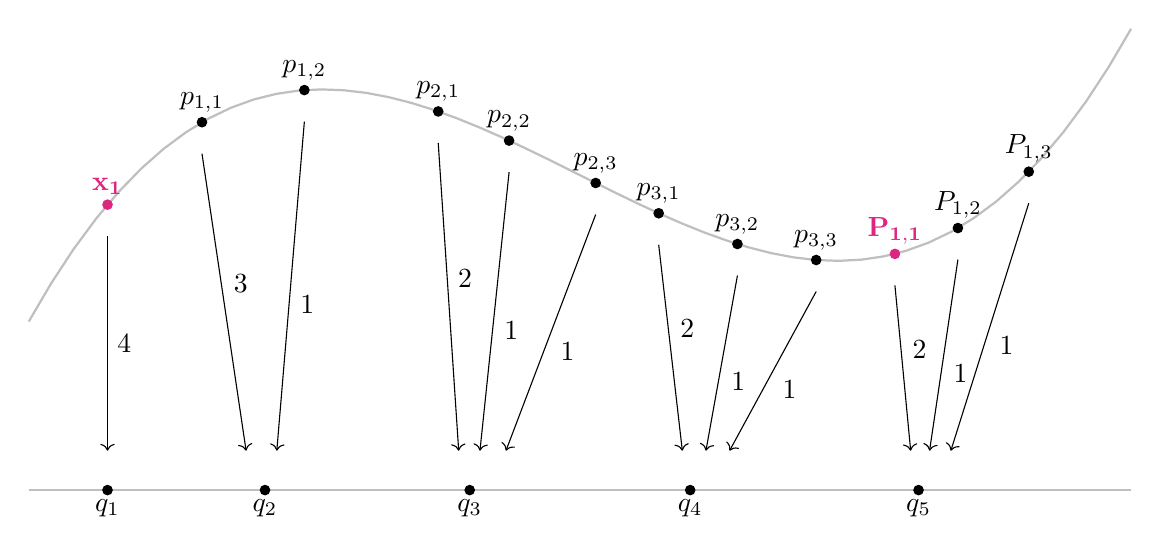
\begin{tikzpicture}
  \draw[domain=-7:7,samples=50,color=gray!50,thick] plot (\x, \x^3/64 - \x/2);
  \foreach \x/\p/\c/\d in {-6/$\mathbf{x_1}$/mypink/4}
  {
    \filldraw[\c] (\x,\x^3/64 - \x/2) circle (0.6mm) node[above] {\p};
    \draw[->] (\x,\x^3/64 - \x/2 - .4) to["\d"] (-6, -3.5);
  }

    \foreach \x/\p/\c/\d in {-4.8/$p_{1,1}$/black/3, -3.5/$p_{1,2}$/black/1}
  {
    \filldraw[\c] (\x,\x^3/64 - \x/2) circle (0.6mm) node[above] {\p};
    \draw[->] (\x,\x^3/64 - \x/2 - .4) to["\d"] (-2.8+.3*\x, -3.5);
  }
  
  \foreach \x/\p/\c/\d in {-1.8/$p_{2,1}$/black/2, -.9/$p_{2,2}$/black/1, .2/$p_{2,3}$/black/1}
  {
    \filldraw[\c] (\x,\x^3/64 - \x/2) circle (0.6mm) node[above] {\p};
    \draw[->] (\x,\x^3/64 - \x/2 - .4) to["\d"] (-1+.3*\x, -3.5);
  }

    \foreach \x/\p/\c/\d in {1/$p_{3,1}$/black/2, 2/$p_{3,2}$/black/1, 3/$p_{3,3}$/black/1}
  {
    \filldraw[\c] (\x,\x^3/64 - \x/2) circle (0.6mm) node[above] {\p};
    \draw[->] (\x,\x^3/64 - \x/2 - .4) to["\d"] (1+.3*\x, -3.5);
  }
  
  \foreach \x/\p/\c/\d in {4/$\mathbf{P_{1,1}}$/mypink/2, 4.8/$P_{1,2}$/black/1, 5.7/$P_{1,3}$/black/1}
  {
    \filldraw[\c] (\x,\x^3/64 - \x/2) circle (0.6mm) node[above] {\p};
    \draw[->] (\x,\x^3/64 - \x/2 - .4) to["\d"] (3+.3*\x, -3.5);
    }

    \draw[domain=-7:7,samples=50,color=gray!50,thick] plot (\x, -4);
  \foreach \x/\q in {-6/$q_1$, -4/$q_2$, -1.4/$q_3$, 1.4/$q_4$, 4.3/$q_5$}
    \filldraw[black] (\x,-4) circle (0.6mm) node[below] {\q};
\end{tikzpicture}

\label{fig:Sab}
  \end{figure}
\end{eg}

\begin{eg}
  \label{eg:Sabns}
  We can specialize to the case where $\a$ is of the simple form
  $\a=\{n,\dots,n\}\cup\{2,\dots,2\}$, where there are $k$ appearances
  of $n$ and $\ell$ appearances of $2$, and $\b=\{t\}$ (the $\b=\emptyset$
  case, which is of particular interest to us, corresponding to $t=1$).
  By Riemann-Hurwitz and Lemma~\ref{lem:Sabdim}, for
  $S_{\{n\}^k\cup\{2\}^{\ell},\{t\}}(\mu)$ to be well-defined,
  \begin{align*}
    d-(\ell(\a)-2)+\sum_{x\in\a}(x-1)+(t-1)=2d &\iff d-(k+\ell-2)+k(n-1)+\ell+t-1=2d \\
    &\iff k(n-2)+1+t=d
  \end{align*}
  and $k+\ell=\ell(\mu)+2$.
  For example in the case $n=3$ and $t=1$, we have $d=k+2$; for any fixed $d$,
  \[S_{\{3\}^{d-2}\cup\{2\}^{\ell(\mu)+4-d},\emptyset}(\mu)\] counts genus $1$ covers
  with a fixed ramification profile $\mu$ and as many other
  points of ramification index $3$ as possible. It is well-defined
  as long as $d-\ell(\mu)\leq 4$.
  In Example~\ref{eg:fourtorsion}, we saw that
  \[
  S_{\{4\}\cup\{2,2\},\emptyset}(4)=N_{(4)}(4)=15.
  \]
  For $n>3$, there are additional
  restrictions on the degree $d$.
  \end{eg}

We will compute the invariants $S_{\a,\b}(\mu)$ as follows. First,
we use our admissible covers technique
and Theorem~\ref{thm:admissible} to establish a recursion (Theorem~\ref{thm:reduceb}) that allows us to remove elements of
$\b$, and we then apply the same
technique to establish another recursion (Theorem~\ref{thm:reducea}) that allows us to remove elements of $\a$; the combination
of these recursions allows us to reduce to the case where $\mu=(d)$ and $\b$ is empty. Finally,
we establish the base case (Theorem~\ref{thm:Sabbase}) using our previously demonstrated genus reduction technique.

While these results in principle provide an algorithm for computing any invariant
$S_{\a,\b}(\mu)$, the recursions involved are too messy to expect a general closed
form solution for these invariants,
even in the special case of interest $\mu=(1^d)$. However, we expect that the special cases
$T_{k,t,a}^{(n)}$ are more tractable, and we will explicitly find a closed form
for the invariants $T_{k,1,1}^{(3)}$ in Proposition~\ref{prop:deg4}.

\section{Reduction of $\b$}

\begin{thm}
  \label{thm:reduceb}
  For $n>0$, if $y>0$, then
  \begin{align*}
    S_{\mathfrak a,\mathfrak b+\{y\}}(\mu, n) &=S_{\mathfrak a,\mathfrak b}(\mu, n-y+1) +\sum_{z\in\mathfrak a}\min(z-1,y-1,n,y+z-n-2)S_{\mathfrak a-\{z\},\mathfrak b+\{y+z-n-2\}}(\mu)
  \end{align*}
  This sum is over $\a$ as a set rather than a multiset, i.e.\ there is
  a single term for each unique value in $\a$.
\end{thm}

\begin{proof}
  Let $k=\ell(\mu)$. We can apply Theorem~\ref{thm:admissible}
  to calculate $W_{1,\sigma,\nu}$ and divide by the normalizing factor
  \[ 
  \prod_{x\in\a+\b+\{y\}}(d-x)!\cdot |\Aut(\a)|\cdot |\Aut(\b+\{y\})|,
  \]
  but for brevity we will instead perform calculations on level of
  $N_{1,\sigma,\nu}$ to avoid writing combinatorial terms that cancel.
  Let $A$ be the following graph,
  with a genus $1$ component containing $x_1,\dots,x_k$ and all but one
  of the other fixed points:

    \begin{figure}[h]
    \caption{Graph $A$ in the reduction of $\b$}
    \centering
                  \begin{tikzpicture}[thick]

  \matrix[amat,nodes=fsnode] (mat1) {$1$\\};

 \matrix[amat,right=4cm of mat1,nodes=ssnode] (mat2) {$0$\\};

 \draw  (mat1-1-1) edge (mat2-1-1);

  % draw legs for left side
 \draw (mat1-1-1) -- +(35:.58) node[anchor=west] {$P_{\ell(\b),1}$}
 (mat1-1-1) -- +(60:.58) node[anchor=south] {$\dots$}
 (mat1-1-1) -- +(100:.58) node[anchor=south] {$P_{2,1}$}
 (mat1-1-1) -- +(285:.58) node[anchor=north] {$(x_1,\dots,x_k)$};

 % draw legs for right side
 \draw  (mat2-1-1) -- +(60:.58) node[anchor=west] {$x_{k+1}$}
 (mat2-1-1) -- +(330:.58) node[anchor=west] {$P_{1,1}$};

                  \end{tikzpicture}
                  \end{figure}

                  Note that $|\Aut(A)|=1$.
We now aim to count admissible covers of graphs $\Gamma\to\Gamma'$ where $\Gamma$ has a $\hat A$-structure and $\hat A$ specializes to $A$.
Recall by Lemma~\ref{lem:branchpoints} that there are two branch points not
  arising from the genus $1$ component.
  
  \begin{figure}[h]
    \caption{First cover $\Gamma\to\Gamma'$ in reduction of $\b$}
    \centering
\begin{tikzpicture}[thick]

  \matrix[amat,nodes=fsnode] (mat1) {$1$\\
    $0$\\
    \vdots \\
  $0$\\};

  \matrix[dmat,left=2cm of mat1] (degrees1) {$d-\sum c_i$\\
    $c_1$\\
    \vdots \\
  $c_r$\\};

 \matrix[amat,right=7cm of mat1,nodes=ssnode] (mat2) {$0$\\
   \vdots\\
   $0$ \\
   $0$\\};
 \matrix[dmat,right=1.5cm of mat2] (degrees2) {$\mu_1$\\
   \vdots\\
   $\mu_k$ \\
 $n$\\};

 \draw  (mat1-1-1) edge["$\mu_1$"] (mat2-1-1)
 (mat1-1-1) edge["$\mu_k$"] (mat2-3-1)
 (mat1-1-1) edge["$n-\sum c_i$"] (mat2-4-1)
 (mat1-2-1) edge["$c_1$"] (mat2-4-1)
 (mat1-4-1) edge["$c_r$"] (mat2-4-1);

  % draw legs for left side
 \draw (mat1-1-1) -- +(95:.58) node[anchor=south] {fixed points};

 % draw legs for right side
 \draw  (mat2-1-1) -- +(30:.58) node[anchor=west] {$x_1$}
 (mat2-3-1) -- +(30:.58) node[anchor=west] {$x_k$}
 (mat2-4-1) -- +(30:.58) node[anchor=west] {$x_{k+1}$};

\end{tikzpicture}
\label{fig:reduceb1}
\end{figure}

    A cover of graphs with $x_1,\dots,x_k$ on the right side looks like Figure~\ref{fig:reduceb1}.
There are two branch points outside the genus $1$ component, which must be the images of
$x_1,\dots,x_k,x_{k+1}$ and of $P_{1,1}$. This means there is no extra ramification on any genus $0$ component, which is why each top right bubble
connects only to the genus $1$ component. The bottom right bubble must have some ramification beyond what is pictured here, which is necessarily
$P_{1,1}$, so our diagram looks like Figure~\ref{fig:reduceb1simplified}.
  As there is no extra ramification outside the genus $1$ component,
  the dimension reduction of $r$ should match the codimension reduction
  corresponding to the removal of $P_{1,1}$, which is $y-1$. So $r=y-1$ and we
  have the first term in the claim, since $H((n),(y,1,\dots),(n-y+1,1,\dots))=1$.


\begin{figure}[h]
  \caption{Simplification of Figure~\ref{fig:reduceb1}}
    \label{fig:reduceb1simplified}
    \centering
  \begin{tikzpicture}[thick]

  \matrix[amat,nodes=fsnode] (mat1) {$1$\\
    $0$\\
    \vdots \\
  $0$\\};

  \matrix[dmat,left=2cm of mat1] (degrees1) {$d-r$\\
    $1$\\
    \vdots \\
  $1$\\};

 \matrix[amat,right=7cm of mat1,nodes=ssnode] (mat2) {$0$\\
   \vdots\\
   $0$ \\
   $0$\\};
 \matrix[dmat,right=1.5cm of mat2] (degrees2) {$\mu_1$\\
   \vdots\\
   $\mu_k$ \\
 $n$\\};

 \draw  (mat1-1-1) edge["$\mu_1$"] (mat2-1-1)
 (mat1-1-1) edge["$\mu_k$"] (mat2-3-1)
 (mat1-1-1) edge["$n-r$"] (mat2-4-1)
 (mat1-2-1) edge["$1$"] (mat2-4-1)
 (mat1-4-1) edge["$1$"] (mat2-4-1);

  % draw legs for left side
 \draw (mat1-1-1) -- +(95:.58) node[anchor=south] {fixed points};

 % draw legs for right side
 \draw  (mat2-1-1) -- +(30:.58) node[anchor=west] {$x_1$}
 (mat2-3-1) -- +(30:.58) node[anchor=west] {$x_k$}
 (mat2-4-1) -- +(30:.58) node[anchor=west] {$x_{k+1}$}
 (mat2-4-1) -- +(330:.58) node[anchor=west] {$P_{1,1}$};

  \end{tikzpicture}
  \end{figure}


  Now consider the case where $x_1,\dots,x_k,x_{k+1}$ are on the left side. In this
  case, the branch points not coming from the genus $1$ component will be
  the image of $P_{1,1}$ and the image of another point $p_{i,1}$ (with ramification index $z\in\mathfrak a$). Consider the possibility that
  $x_1,\dots,x_k$ are not all on the genus $1$ component.
    This would require the genus $0$ on the right side to have multiple branch points contributing
  $e$ ramification,
  but $P_{1,1}$ cannot live on this component (because of the stabilization condition), a contradiction.
  Therefore, $x_1,\dots,x_k$ all live on the genus $1$ component.

  \begin{figure}[h]
    \caption{$\Gamma\to\Gamma'$ with $x_1,\dots,x_1$ not all on genus $1$ vertex}
  \begin{tikzpicture}[thick]

    \matrix[amat,nodes=fsnode] (mat1) {$0$\\
      $1$\\};

    \matrix[amat,right=2cm of mat1,nodes=ssnode] (mat2) {$0$\\};

      \matrix[dmat,left=1cm of mat1] (degrees1) {$\mu_1$\\
    $d-n-\mu_1$\\};

            \matrix[dmat,right=0.5cm of mat2] (degrees2) {$e$\\};
  
 \draw  (mat1-1-1) edge["$\mu_1$"] (mat2-1-1)
 (mat1-2-1) edge["$e-\mu_1$"] (mat2-1-1);

  % draw legs for left side
 \draw (mat1-1-1) -- +(120:.58) node[anchor=south] {$x_1$}
 (mat1-2-1) -- +(120:.58) node[anchor=south] {$x_2,\dots,x_k$};

   % draw legs for right side
 \draw (mat2-1-1) -- +(100:.58) node[anchor=south] {$e$ ramif};


  \end{tikzpicture}
  \end{figure}

  Moreover the points $P_{1,1}$ and $p_{i,1}$ cannot lie on separate components, because the diagram in Figure~\ref{fig:nocompletion1} cannot be completed.

  \begin{figure}[h]
    \caption{Cover $\Gamma\to\Gamma'$ with $P_{1,1}$ and $p_{i,1}$ on separate components}
    \centering
        \begin{tikzpicture}[thick]

  \matrix[amat,nodes=fsnode] (mat1) {$1$\\
    $0$\\};

  \matrix[dmat,left=2cm of mat1] (degrees1) {$d-n$\\
    $n$\\};

 \matrix[amat,right=3cm of mat1,nodes=ssnode] (mat2) {$0$\\
   $0$\\};
 \matrix[dmat,right=1.5cm of mat2] (degrees2) {$z$\\
   $y$\\};

 \draw  (mat1-2-1) edge["$y$"] (mat2-2-1);

  % draw legs for left side
 \draw (mat1-1-1) -- +(115:.58) node[anchor=south] {fixed points}
 (mat1-1-1) -- +(260:.58) node[anchor=north] {$x_1,\dots,x_k$}
 (mat1-2-1) -- +(260:.58) node[anchor=east] {$x_{k+1}$};

   % draw legs for right side
 \draw (mat2-1-1) -- +(75:.58) node[anchor=south] {$p_{i,1}$}
 (mat2-2-1) -- +(265:.58) node[anchor=north] {$P_{1,1}$};


        \end{tikzpicture}
        \label{fig:nocompletion1}
        \end{figure}

  Therefore $P_{1,1}$ and $p_{i,1}$ lie on the same genus $0$ component, all other genus $0$ components on the right side have degree $1$,
  and we end up with a cover described in Figure~\ref{fig:reduceb2}.

    \begin{figure}[h]
    \caption{Second cover $\Gamma\to\Gamma'$ in reduction of $\b$}
    \centering
        \begin{tikzpicture}[thick]

  \matrix[amat,nodes=fsnode] (mat1) {$1$\\
    $0$\\};

  \matrix[dmat,left=2cm of mat1] (degrees1) {$d-n$\\
    $n$\\};

 \matrix[amat,right=3cm of mat1,nodes=ssnode] (mat2) {$0$\\
   \vdots\\
   $0$ \\
   $0$\\};
 \matrix[dmat,right=1.5cm of mat2] (degrees2) {$1$\\
   \vdots\\
   $1$ \\
   $e+n$\\};

 \draw  (mat1-1-1) edge["$1$"] (mat2-1-1)
 (mat1-1-1) edge["$1$"] (mat2-3-1)
 (mat1-1-1) edge["$e$"] (mat2-4-1)
 (mat1-2-1) edge["$n$"] (mat2-4-1);

  % draw legs for left side
 \draw (mat1-1-1) -- +(115:.58) node[anchor=south] {fixed points}
 (mat1-1-1) -- +(260:.58) node[anchor=north] {$x_1,\dots,x_k$}
 (mat1-2-1) -- +(260:.58) node[anchor=north] {$x_{k+1}$};

   % draw legs for right side
 \draw (mat2-4-1) -- +(75:.58) node[anchor=south] {$P_{1,1}$}
 (mat2-4-1) -- +(265:.58) node[anchor=north] {$p_{i,1}$};


        \end{tikzpicture}
        \label{fig:reduceb2}
        \end{figure}

        By Riemann-Hurwitz for the bottom-right component, 
        \[
        (e+n-2)+(y-1)+(z-1)=2(e+n)-2\implies y+z-2=e+n\implies e=y+z-n-2.
        \]
        By our calculation of $H((y+z-n-2,n),(z,1,\dots),(y,1,\dots))$ (and noting that
        we should multiply by $2$ if $y+z-n-2=n$, since the corresponding edges should be
        distinguished), we end up with the term in the claim.
        
\end{proof}

\section{Reduction of $\a$}
\begin{thm}
  \label{thm:reducea}
  For $n>0$,
  \begin{align*}
    S_{\a,\b}&(\mu, n, m) = \sum_{z\in\mathfrak a,\ z\leq n+m}\min(n,m,z-1,n+m-z+1)S_{\a-\{z\},\b}(\mu,n+m-z+2) \\
    &+\sum_{z_1,z_2\in\a-\{2\}}\hat H((z_1+z_2-n-m-3,n,m),(z_1,1,\dots),(z_2,1,\dots))S_{\a-\{z_1,z_2\},\b+\{z_1+z_2-n-m-3\}}(\mu)
  \end{align*}
\end{thm}
Here $\hat H$ means  ``multiply by $|\Aut(n,m,z_1+z_2-n-m-3)|/|\Aut(z_1,z_2)|$''.

\begin{proof}
    We consider diagrams which stabilize to a genus $1$ curve containing $x_1,\dots,x_k$ and all 
  of the other fixed points, attached to a genus $0$ tail containing $q$ (with ramification index $n$) and $r$
  (with ramification index $m$).
  
  If $x_1,\dots,x_k,q,r$ are on the right side, then there is one more branch point arising as the image of some $s$ (with
  ramification index $z$). Suppose $q$ and $r$ are on different components, as in Figure~\ref{fig:reducea1}.
  (Without loss of generality, we suppose the component containing $q$ is the one that connects to the genus $1$.)
  There is extra ramification on both the component containing $q$ and the lower left component, a contradiction. Therefore
  $q$ and $r$ lie on the same component, and our picture must look like Figure~\ref{fig:reducea2}.

  \begin{figure}[h]
    \caption{Cover $\Gamma\to\Gamma'$ with $q$ and $r$ on different components}
  \begin{tikzpicture}[thick,amat/.style={matrix of nodes,nodes in empty cells,
  row sep=1.0em,rounded corners,
  nodes={draw,solid,circle,minimum size=0.8cm}},
  dmat/.style={matrix of nodes,nodes in empty cells,row sep=1.0em,nodes={minimum size=0.8cm},draw=myred}]

  \matrix[amat,nodes=fsnode] (mat1) {$1$\\
    $0$\\};

 \matrix[amat,right=4cm of mat1,nodes=ssnode] (mat2) {$0$\\
   \vdots\\
   $0$ \\
   $0$\\
 $0$\\};

 \draw  (mat1-1-1) edge["$\mu_1$"] (mat2-1-1)
 (mat1-1-1) edge["$\mu_k$"] (mat2-3-1)
 (mat1-1-1) edge["$c$"] (mat2-4-1)
 (mat1-2-1) edge["$e$"] (mat2-4-1)
 (mat1-2-1) edge["$m$"] (mat2-5-1);

  % draw legs for left side
 \draw (mat1-1-1) -- +(95:.58) node[anchor=south] {fixed points};

 % draw legs for right side
 \draw  (mat2-1-1) -- +(30:.58) node[anchor=west] {$x_1$}
 (mat2-3-1) -- +(30:.58) node[anchor=west] {$x_k$}
 (mat2-4-1) -- +(30:.58) node[anchor=west] {$q$}
 (mat2-5-1) -- +(30:.58) node[anchor=west] {$r$};

  \end{tikzpicture}
      \label{fig:reducea1}
  \end{figure}

  \begin{figure}[h]
    \caption{First cover $\Gamma\to\Gamma'$ in reduction of $\a$}
    \centering
    \begin{tikzpicture}[thick, amat/.style={matrix of nodes,nodes in empty cells,
  row sep=.7em,rounded corners,
  nodes={draw,solid,circle,minimum size=0.8cm}},
  dmat/.style={matrix of nodes,nodes in empty cells,row sep=.7em,nodes={minimum size=0.8cm},draw=myred}]

  \matrix[amat,nodes=fsnode] (mat1) {$1$\\
    $0$\\
    \vdots\\
    $0$\\};

    \matrix[dmat,left=1cm of mat1] (degrees1) {$d-e$\\
    $1$\\
    \vdots \\
  $1$\\};


 \matrix[amat,right=5cm of mat1,nodes=ssnode] (mat2) {$0$\\
   \vdots\\
   $0$ \\
   $0$\\};

     \matrix[dmat,right=1cm of mat2] (degrees2) {$\mu_1$\\
    \vdots \\
    $\mu_k$\\
     $n+m$\\};

 \draw  (mat1-1-1) edge["$\mu_1$"] (mat2-1-1)
 (mat1-1-1) edge["$\mu_k$",bend left=10] (mat2-3-1)
 (mat1-1-1) edge["$n+m-e$",font=\scriptsize] (mat2-4-1)
 (mat1-2-1) edge["$1$",bend right=2] (mat2-4-1)
 (mat1-4-1) edge["$1$"] (mat2-4-1);

  % draw legs for left side
 \draw (mat1-1-1) -- +(95:.58) node[anchor=south] {fixed points};

 % draw legs for right side
 \draw  (mat2-1-1) -- +(30:.58) node[anchor=west] {$x_1$}
 (mat2-3-1) -- +(30:.58) node[anchor=west] {$x_k$}
 (mat2-4-1) -- +(30:.58) node[anchor=west] {$q$}
 (mat2-4-1) -- +(50:.58) node[anchor=west] {$r$}
 (mat2-4-1) -- +(300:.58) node[anchor=west] {$s$};

    \end{tikzpicture}
        \label{fig:reducea2}
    \end{figure}

    By Riemann-Hurwitz for the lower right component,
    \[
    (n+m-e-1)+(n+m-2)+(z-1)=2(n+m)-2\implies e=z-2
    \]
    yielding the first term in the claim using our calculation of Hurwitz numbers to simplify
    $H((n,m),(z,1,\dots),(n+m-z+2,1,\dots))$.

    If $x_1,\dots,x_k,q,r$ are on the left side, then there are two branch points arising as the images of $s_1$ (with
    ramification index $z_1$) and $s_2$ (with ramification index $z_2$). By logic similar to the last proof, the
    $x_1,\dots,x_k$ all lie on the genus $1$ component.

    Consider the possibility that $q$ and $r$ lie on the same component, depicted in Figure~\ref{fig:qrsame}.

    \begin{figure}[h]
      \caption{Cover $\Gamma\to\Gamma'$ in reduction of $\a$ with $q$ and $r$ on the same component}
      \centering
      \begin{tikzpicture}[thick]

  \matrix[amat,nodes=fsnode] (mat1) {$1$\\
    $0$\\};

 \matrix[amat,right=7cm of mat1,nodes=ssnode] (mat2) {$0$\\
   \vdots\\
   $0$ \\
 $0$\\};

 \draw  (mat1-1-1) edge["$1$"] (mat2-1-1)
 (mat1-1-1) edge["$1$"] (mat2-3-1)
 (mat1-1-1) edge["$c$"] (mat2-4-1)
 (mat1-2-1) edge["$n+m$"] (mat2-4-1);

  % draw legs for left side
 \draw (mat1-1-1) -- +(95:.58) node[anchor=south] {fixed points}
 (mat1-1-1) -- +(270:.58) node[anchor=north] {$x_1,\dots,x_k$}
 (mat1-2-1) -- +(270:.58) node[anchor=north] {$q$}
 (mat1-2-1) -- +(255:.58) node[anchor=north] {$r$};

      \end{tikzpicture}
      \label{fig:qrsame}
      \end{figure}

      There must be at least one additional branch point from the lower left component and at least two additional branch
      points from the lower right component, a contradiction. Therefore, $q$ and $r$ lie on separate components as in
      Figure~\ref{fig:qrdiff}.

      \begin{figure}[h]
        \caption{Cover $\Gamma\to\Gamma'$ in reduction of $\a$ with $q$ and $r$ on separate components}
        \centering
          \begin{tikzpicture}[thick]

  \matrix[amat,nodes=fsnode] (mat1) {$1$\\
    $0$\\
    $0$\\};

    \matrix[dmat,left=1cm of mat1] (degrees1) {$d-n-m$\\
    $n$\\
  $m$\\};


 \matrix[amat,right=4cm of mat1,nodes=ssnode] (mat2) {$0$\\
   \vdots\\
   $0$ \\
   $0$\\};

     \matrix[dmat,right=1cm of mat2] (degrees2) {$1$\\
    \vdots \\
    $1$\\
     $c+n+m$\\};

 \draw  (mat1-1-1) edge["$1$"] (mat2-1-1)
 (mat1-1-1) edge["$1$"] (mat2-3-1)
 (mat1-1-1) edge["$c$"] (mat2-4-1)
 (mat1-2-1) edge["$n$"] (mat2-4-1)
 (mat1-3-1) edge["$m$"] (mat2-4-1);

  % draw legs for left side
 \draw (mat1-1-1) -- +(95:.58) node[anchor=south] {fixed points}
 (mat1-1-1) -- +(245:.58) node[anchor=north] {$x_1,\dots,x_k$}
 (mat1-2-1) -- +(245:.58) node[anchor=north] {$q$}
 (mat1-3-1) -- +(245:.58) node[anchor=north] {$r$};

 % draw legs for right side
 \draw  (mat2-4-1) -- +(30:.58) node[anchor=west] {$s_1$}
 (mat2-4-1) -- +(300:.58) node[anchor=west] {$s_2$};

          \end{tikzpicture}
          \label{fig:qrdiff}
          \end{figure}
          
          By Riemann-Hurwitz for the lower-right component,
          \[
          (c+n+m-3)+(z_1-1)+(z_2-1)=2(c+n+m)-2\implies c=z_1+z_2-n-m-3
          \]
          yielding the second term of the claim. The additional factors arise because
          the edges from the bottom right component should be distinguished, while $s_1$ and
          $s_2$ should not be distinguished.
\end{proof}

It remains to calculate $S_{\{a_1,a_2,a_3\},\emptyset}(d)$ as a base case:

\begin{thm}
  \label{thm:Sabbase}
  When $\a=\{a_1,a_2,a_3\}$, $S_{\a,\emptyset}(d)$ is given by
  \[
  S_{\a,\emptyset}(d)=\sum_{i=1}^3\sum_{e+f=d-a_i+2}X_{i}Y_{e,f}\]
  where
  \begin{align*}
    X_{i,e,f}=\frac{2(a_j+a_k-2) H((d),(a_i,1,\dots),(e,f,1,\dots))}{(a_i-2)!|\Aut(a_1,a_2,a_3)|}\cdot \\
    &H((e,f),(a_j,1,\dots),(a_k,1,\dots)) |\Aut(e,f,1^{d-e-f})|,
  \end{align*}
  and $\{1,2,3\}=\{i,j,k\}$.
\end{thm}
\begin{proof}
  We will want to calculate $W_{(a_1,1,\dots),(a_2,1,\dots),(a_3,1,\dots)}(d)$ and then divide by \[(d-a_1)!(d-a_2)!(d-a_3)!|\Aut(a_1,a_2,a_3)|\]
  Let $A$ be the standard graph for genus reduction; we will apply Theorem~\ref{thm:admissible}. Any admissible cover of graphs $\Gamma\to\Gamma'$ will
  have a single genus $0$ component on the left side containing
  $x_1$ with a double edge to a genus $0$ component on the right side.
  By Riemann-Hurwitz, the left component has another ramified
  point $p_{i,1}$, and the genus $0$ component to which it has a double
  edge has two ramified points $p_{j,1}$ and $p_{k,1}$. Our picture looks like Figure~\ref{fig:Sabbasecase}.

  \begin{figure}[h]
    \caption{Cover $\Gamma\to\Gamma'$ in the computation of $S_{\a,\emptyset}(d)$}
    \centering
            \begin{tikzpicture}[thick]

  \matrix[amat,nodes=fsnode] (mat1) {$0$\\};

    \matrix[dmat,left=1cm of mat1] (degrees1) {$d$\\};


 \matrix[amat,right=4cm of mat1,nodes=ssnode] (mat2) {$0$\\
      $0$\\
      $\vdots$\\
  $0$\\};

 \matrix[dmat,right=1cm of mat2] (degrees2) {$e+f$\\
   $1$ \\
    \vdots \\
    $1$\\};

 \draw  (mat1-1-1) edge["$e$",bend left] (mat2-1-1)
 (mat1-1-1) edge["$f$"] (mat2-1-1)
 (mat1-1-1) edge["$1$"] (mat2-2-1)
 (mat1-1-1) edge["$1$"] (mat2-4-1);

  % draw legs for left side
 \draw (mat1-1-1) -- +(95:.58) node[anchor=south] {$x_1$}
 (mat1-1-1) -- +(245:.58) node[anchor=north] {$p_{i,1}$};

 % draw legs for right side
 \draw  (mat2-1-1) -- +(30:.58) node[anchor=west] {$p_{j,1}$}
 (mat2-1-1) -- +(330:.58) node[anchor=west] {$p_{k,1}$};
 

            \end{tikzpicture}
            \label{fig:Sabbasecase}
            \end{figure}

            Riemann-Hurwitz says that
            \[
            (a_i-1)+(d-1)+(e+f-2)=2d-2\iff e+f=d-a_i+2
            \]
            and
            \[
            (e+f-2)+(a_j-1)+(a_k-1)=2(e+f)-2\iff a_i+a_j+a_k=d+4
            \]
            where this second equality is already known.

            The number of choices for points not marked in this
            picture is computed as follows: first,
            there are $\binom{d-a_j}{e+f-a_j}$ choices
            for which of $p_{j,2},\dots$ to place on the top right component,
            and similarly $\binom{d-a_k}{e+f-a_k}$ choices
            for which of $p_{k,2},\dots$ to place on the top right component.
            Once these are fixed, each other genus $0$ component
            on the right can be identified by which element of
            $p_{j,2},\dots$ it contains, and there are
            then $(d-e-f)!$ choices for placement of
            the remaining $p_{k,2},\dots$ among
            these components.

            Therefore, the contribution to the right side of Theorem~\ref{thm:admissible} is
            \begin{align*}
              &\frac{c_{\Gamma}}{|\Aut(\Gamma)|}\binom{d-a_j}{e+f-a_j}\binom{d-a_k}{e+f-a_k}(d-e-f)!\cdot \\
              &\overline H((d),(a_i,1,\dots),(e,f,1,\dots))\cdot\overline H((e,f),(a_j,1,\dots),(a_k,1,\dots)) \\
              &=\frac{e+f}{|\Aut(e,f)|}\cdot\frac{(d-a_j)!(d-a_k)!}{(e+f-a_j)!(e+f-a_k)!((d-e-f)!)^2}\cdot (d-e-f)!\cdot \\
              & H((d),(a_i,1,\dots),(e,f,1,\dots))(d-a_i)!|\Aut(e,f,1,\dots)|H((e,f),(a_j,1,\dots),(a_k,1,\dots))\cdot \\
              &(e+f-a_j)!(e+f-a_k)!|\Aut(e,f)| \\
              &=\frac{(e+f)\prod\limits_{\ell=1}^3(d-a_{\ell})!\cdot H((d),(a_i,1,\dots),(e,f,1,\dots))H((e,f),(a_j,1,\dots),(a_k,1,\dots)) }{(d-e-f)!} \cdot \\
              &\hspace*{0.3in}|\Aut(e,f,1,\dots)|
            \end{align*}
            and so the contribution to $S_{\a,\emptyset}(d)$ is double this
            (given $|\Aut(A)|=2$) divided by the normalizing factor, i.e.
            \[
            \frac{2(e+f)\cdot H((d),(a_i,1,\dots),(e,f,1,\dots))\cdot H((e,f),(a_j,1,\dots),(a_k,1,\dots))\cdot|\Aut(e,f,1,\dots)|}{(d-e-f)!\cdot |\Aut(a_i,a_j,a_k)|}
            \]
            Since $e+f=a_j+a_k-2$ and $d-e-f=a_i-2$, this proves the claim.
\end{proof}
\begin{eg}
  We can use this formula to prove that $S_{\{4,2,2\},\emptyset}(4)=15$, as was previously shown in
  Example~\ref{eg:genusreduction}.
  The $i=1$ term is
  \[
  \frac{2(2+2-2)H((4),(4),(1,1,1,1))H((1,1),(2),(2))|\Aut(1,1,1,1)|}{2!|\Aut(4,2,2)|} =\frac{2\cdot 2\cdot \frac 14\cdot \frac 12\cdot 4!}{2\cdot 2}=3,
  \]
  while both the $i=2$ and $i=3$ terms are
  \[
  \frac{2(4)H((4),(2,1,1),(3,1))H((3,1),(4),(2,1,1))|\Aut(3,1)|}{0!\cdot 2}=\frac{2\cdot 4\cdot 1\cdot 1\cdot 1}{2}=4
  \]
  (corresponding to $(e,f)=(3,1)$) plus
  \[
  \frac{2(4)H((4),(2,1,1),(2,2))H((2,2),(4),(2,1,1))|\Aut(2,2)|}{0!\cdot 2}=\frac{2\cdot 4\cdot \frac 12\cdot \frac 12\cdot 2}{2}=2
  \]
  (corresponding to $(e,f)=(2,2)$). Adding these together yields
  \[
  3+2(4+2)=15.
  \]
  \end{eg}

\section{Applying recursions}

In order to solve our recursions, we need the following result:

\begin{thm}
  Every invariant $S_{\a,\b}(\mu)$ can be computed by
  a finite
  sequence of applications of Theorems~\ref{thm:reduceb}, \ref{thm:reducea} and \ref{thm:Sabbase}.
  \end{thm}
\begin{proof}
  Let $X=\{(a,b,k)\}=\Z_{\geq 0}^3$ with the total order where
  $(a,b,k)<(a',b',k')$
  if:
  \begin{itemize}
  \item $k<k'$, or
  \item $k=k'$ and $b<b'$, or
    \item $k=k'$, $b=b'$, and $a<a'$
  \end{itemize}
  We will prove by induction on $(a,b,k)$, under this order, that
  any $S_{\a,\b}(\mu)$ with $\ell(\a)=a$, $\ell(\b)=b$, and $\ell(\mu)=k$
  can be computed by a finite sequence of applications
  of Theorems~\ref{thm:reduceb}, \ref{thm:reducea} and \ref{thm:Sabbase}.
  Induction is possible here because for invariants $S_{\a,\b}(\mu)$
  we require $\ell(\mu)\leq d$ and $\ell(\a),\ell(\b)\leq 2d$, implying
  that each $(a,b,k)$ is greater than only finitely many triples
  of interest.
  
  As a base case, if $(a,b,k)<(\infty,0,1)$, then
  this means either $k=0$ (in which case
  our convention is $S_{\a,\b}(\emptyset)=0$) or $k=1$ and $b=0$
  (in which case we can directly apply Theorem~\ref{thm:Sabbase} to find
  $S_{\a,\emptyset}(d)$).

  Now suppose that $(a,b,k)>(\infty,0,1)$
  and that the theorem is true for any $(a',b',k')<(a,b,k)$. There are two cases:
  \begin{enumerate}
  \item If $k>1$, then Theorem~\ref{thm:reducea} reduces $S_{\a,\b}(\mu)$ to
    a sum of terms involving triples less than $(a,b,k)$.
  \item If $k=1$ and $b>0$, then Theorem~\ref{thm:reduceb} reduces
    $S_{\a,\b}(\mu)$ to a sum of terms involving triples less than $(a,b,k)$.
  \end{enumerate}
  In either case the result is proven.
\end{proof}

\begin{eg}
  We compute the value of $S_{\{3,2,2,2\},\{2\}}(3,1)$:
  \begin{align*}
    S_{\{3,2,2,2\},\{2\}}(3,1) &= S_{\{3,2,2,2\},\emptyset}(3,0)+\sum_{z\in\{3,2,2,2\}}S_{\{3,2,2,2\}-\{z\},\{z-1\}}(3) \tag*{(Theorem~\ref{thm:reduceb})} \\
    &=0+S_{\{2,2,2\},\{2\}}(3)+3S_{\{3,2,2\},\emptyset}(3) \\
    &=S_{\{2,2,2\},\emptyset}(2)+3S_{\{3,2,2\},\emptyset}(3)
  \end{align*}
%  (TODO: apply Theorem 7 for base case)
\end{eg}

In general, the application of these recursions is somewhat complex and
does not seem to lead to a closed form. However, we can make headway
by considering a slight modification of the family of invariants
in Example~\ref{eg:Sabns}.


\section{$T_{k,1,1}^{(n)}$}

\begin{dfn}
  Define
  \[
  T_{k,t,a}^{(n)}=S_{\{n\}^k\cup\{2\}^{\ell},\{t\}}(a,1^b)
  \]
  where $b=k(n-2)+1+t-a$ so that $a+b=d=k(n-2)+1+t$, and
  by Riemann-Hurwitz,
  \[
  2d=k(n-1)+\ell+t-1+a-1\implies \ell=kn-3k+4-a+t
  \]
  Note that $T_{k,1,a}^{(n)}$
  recovers the notion of Example~\ref{eg:Sabns} for $\mu=(a,1^b)$.
  \end{dfn}

Theorems~\ref{thm:reduceb} and \ref{thm:reducea} specialize to recursions
within the family $T_{k,t,a}^{(n)}$:
\begin{itemize}
\item $T_{k,t,a}^{(n)}=T_{k,1,a-t+1}^{(n)}+\cdot\min(n-1,t-1,a,t+n-a-2)T_{k-1,t+n-a-2,1}^{(n)}+ T_{k,t-a,1}^{(n)}$
\item For $a<k(n-2)+2$, \[T_{k,1,a}^{(n)}=T_{k,1,a+1}^{(n)}+T_{k-1,1,a+3-n}^{(n)}+\hat H((a,1,2n-a-4),(n,1,\dots),(n,1,\dots))T_{k-2,2n-a-4,1}^{(n)}\] if $a+1\geq n$ and
  \[T_{k,1,a}^{(n)}=T_{k,1,a+1}^{(n)}+\hat H((a,1,2n-a-4),(n,1,\dots),(n,1,\dots))T_{k-2,2n-a-4,1}^{(n)}\]
  if $a+1<n$.
\end{itemize}
Theorem~\ref{thm:Sabbase} also gives us a formula for
$T_{k,1,k(n-2)+2}$.

We pay particular attention to two special subfamilies:
$V_{k,t}^{(n)}=T_{k,t,1}^{(n)}$ (where $\mu=(1^d)$) and $U_{k,a}^{(n)}=T_{k,1,a}^{(n)}$
(where $\b=\{1\}$ or equivalently, $\b=\emptyset$). 

For these subfamilies we have:
\begin{itemize}
\item $V_{k,t}^{(n)}=V_{k,t-1}^{(n)}+V_{k-1,t+n-3}^{(n)}$ for $t>1$
  \item For $a<k(n-2)+2$, \[U_{k,a}^{(n)}=U_{k,a+1}^{(n)}+(a+1\geq n)U_{k-1,a+3-n}^{(n)}+\hat H((a,1,2n-a-4),(n,1,\dots),(n,1,\dots)) V_{k-2,2n-a-4}\]
\end{itemize}

The overlap of these two subfamilies, $T_{k,1,1}^{(n)}$, is of special interest:

Letting $d=k(n-2)+2$,
given a generic $d$-pointed genus $1$ curve $(E,x_1,\dots,x_d)$,
$T_{k,1,1}^{(n)}$ is the number of covers $(E,x_1,\dots,x_d)\to(\P^1,0)$
with $k$ unspecified points of $E$ having ramification index $n$.
Equivalently, given a generic genus $1$ curve $E\subset \P^{d-1}$,
$T_{k,1,1}^{(n)}$ is the number of fibers of a generic projection
$(\P^{d-1})^*\dashrightarrow\P^{d-2}$ containing $k$ distinct points
of $X_{(n,1,\dots,1)}$ (Proposition~\ref{prop:direct}).
We have
seen that an analogous family in the ``all twos'' case, $N_{(2^k),(2^k)}(1^{2k})$,
grows exponentially in $k$ (Corollary~\ref{cor:twos}), and are interested
in the growth rate of $T_{k,1,1}^{(n)}$ for $n$ fixed.



We focus in particular on the case where $n=3$:
\[
U_{k,a}^{(3)}=U_{k,a+1}^{(3)}+U_{k-1,a}^{(3)}\text{ for }1<a<k+2,\qquad U_{k,1}^{(3)}=U_{k,2}^{(3)}+U_{k-2,1}^{(3)}
\]

\begin{prop}
  \label{prop:deg4}
  For $k\geq 1$,
  \[
  U_{k,1}^{(3)}=T_{k,1,1}^{(3)}=f(k)
  \]
  where
  \[
  f(k) = \frac{(k+2)(k+1)(2(k+1)^2+1)}{6}
  \]
\end{prop}
\begin{proof}
  First, we can use Theorem~\ref{thm:Sabbase} to compute:
  \begin{itemize}
  \item $U_{3,5}=16$
  \item $U_{2,4}=20$
  \item $U_{1,3}=8$
    \item $U_{0,2}=1$
    \end{itemize}
  Note that $U_{k,a}=0$ if $a\geq 6$, since
  $\ell=(k+2-a)+3-k=5-a<0$. Therefore,
  \[
  U_{k,5}^{(3)}-U_{k-1,5}^{(3)}=U_{k,6}^{(3)}=0
  \]
  implying that $U_{k,5}^{(3)}$ when
  defined is constant and always equal to $U_{3,5}^{(3)}=16$.

  Next,
  \[
  U_{k,4}^{(3)}-U_{k-1,4}^{(3)}=U_{k,5}^{(3)}=16
  \]
  so $U_{k,4}^{(3)}$ is linear in $k$ with slope $16$, and since $U_{2,4}^{(3)}=20$,
  this implies $U_{k,4}^{(3)}=16k-12$ where defined.

  For $a=3$,
  \[
  U_{k,3}^{(3)}-U_{k-1,3}^{(3)}=U_{k,4}^{(3)}=16k-12
  \]
  so given that $U_{1,3}^{(3)}=8$,
  \[
  U_{k,3}^{(3)}=8+\sum_{j=2}^k(16j-12)=8+16\left(\frac{j(j+1)}2-1\right)-12(k-1)=8k^2-4k+4
  \]
  where defined. For $a=2$,
  \[
  U_{k,2}^{(3)}-U_{k-1,2}^{(3)}=U_{k,3}^{(3)}=8k^2-4k+4
  \]
  so given that $U_{0,2}=1$,
  \[
  U_{k,2}^{(3)}=1+\sum_{j=1}^k(8j^2-4j+4)=1+8\cdot\frac{k(k+1)(2k+1)}{6}-4\cdot\frac{k(k+1)}{2}+4k=\frac{8k^3}{3}+2k^2+\frac{10k}{3}+1
  \]
  where defined. Finally, $U_{k,1}^{(3)}-U_{k-2,1}^{(3)}=U_{k,2}^{(3)}$
  and $U_{0,1}^{(3)}=1$, $U_{1,1}^{(3)}=9$. There is a unique
  function $k\mapsto U_{k,1}^{(3)}$ satisfying these conditions,
  so we need only show that these conditions hold for the quartic $f(k)$:
  \begin{align*}
    f(k)-f(k-2)&=\frac{(k+2)(k+1)(2(k+1)^2+1)}{6}-\frac{k(k-1)(2(k-1)^2+1)}{6} \\
    &=\frac{2k^4+10k^3+19k^2+17k+6}{6}-\frac{2k^4-6k^3+7k^2-3k}{6} \\
    &=\frac{16k^3+12k^2+20k+6}{6} \\
    &=U_{k,2}^{(3)}
  \end{align*}
  and $f(0)=\frac{(2)(1)(3)}{6}=1$, $f(1)=\frac{(3)(2)(2\cdot 2^2+1)}{6}=9$.

\end{proof}

For $n>3$, it becomes more difficult to solve the recurrence relations,
since $U_{k,a}^{(n)}$ is now expressed in terms of invariants $U$ and $V$,
and thus we need to understand both $U$ and $V$.
For instance when $n=4$, we have:
\begin{itemize}
\item $U_{k,1}^{(4)}=U_{k,2}^{(4)}+V_{k-2,3}^{(4)}$
\item $U_{k,2}^{(4)}=U_{k,3}^{(4)}+2V_{k-2,2}^{(4)}$
  \item $U_{k,3}^{(4)}=U_{k,4}^{(4)}+U_{k-1,2}^{(4)}+V_{k-2,1}^{(4)}$
\item $U_{k,a}^{(4)}=U_{k,a+1}^{(4)}+U_{k-1,a-1}^{(4)}$ for $3<a<2k+2$
  \item $V_{k,t}^{(4)}=V_{k,t-1}^{(4)}+V_{k-1,t+1}^{(4)}$ for $t>1$
\end{itemize}
By the fact that the number of simple ramification profiles
for $U_{k,a}^{(n)}$ is
$\ell=k(n-3)+5-a\geq 0$, we have
\[
U_{k,k(n-3)+5}^{(n)}=U_{k,k(n-3)+6}^{(n)}+U_{k-1,(k-1)(n-3)+5}^{(n)}
\]
and since the first term vanishes, $U_{k,k(n-3)+5}^{(n)}$ is a constant
function of $k$. For $s$ fixed and $k$
sufficiently large, $U_{k,k(n-3)+5-s}^{(n)}$ will be a degree $s$ function
of $k$ (since its first differences are the values $U_{k,k(n-3)+5-(s-1)}$).
This explains the quartic form for $U_{k,1}^{(3)}$, but
for $n>3$, we cannot expect $U_{k,1}^{(n)}$ to be polynomial.

\iffalse
The last equation yields the following result:
\begin{prop}
  For $k\geq 0$ and $t>1$,
  \[
  V_{k,t}^{(4)}=a_0(t)V_{k,1}^{(4)}+a_1(t)V_{k-1,1}^{(4)}+a_2(t)V_{k-2,1}^{(4)}+\dots+a_{k-1}(t)V_{1,1}^{(4)}+a_k(t)V_{0,1}^{(4)}=\sum_{n=0}^k a_n(t)V_{k-n,1}^{(4)}
  \]
  where
  \[
  a_k(t)=\#\{(r_1,\dots,r_k):r_k\leq t+1,\ 3\leq r_i\leq r_{i+1}+1\text{ for }1\leq i<k\}
  \]
\end{prop}
\begin{proof}
  TODO
\end{proof}
\fi

We provide the following table of values of some $T_{k,1,1}^{(n)}$ in general:

  \begin{table}[h]
    \caption{Table of values of $T_{k,1,1}^{(n)}$}
    \centering
    ~\\
  \begin{tabular}{l|l|l|l|l|l|l|}
    & $k=0$ & $k=1$ & $k=2$ & $k=3$ & $k=4$ & $k=5$ \\ \hline
    $n=3$ & $1$ & $9$ & $38$ & $110$ & $255$ & $511$ \\ \hline
    $n=4$ & $1$ & $16$ & $114$ & $608$ & $2865$ & $12672$ \\ \hline
    $n=5$ & $1$ & $25$ & $252$ & $1969$ & $14105$ & $97308$ \\ \hline
    $n=6$ & $1$ & $36$ & $470$ & $4844$ & $46665$ & $438284$ \\ \hline
\end{tabular}
  \end{table}

  Note that $T_{1,1,1}^{(n)}=N_{(n)}(1^n)=n^2$, corresponding
  to a count of the $n$-torsion points in an elliptic curve.

One next step would
be to more fully study the asymptotics of $T_{k,t,a}^{(n)}$, using
the theory of linear recursions.
Another direction might be to study invariants $N_{g,\sigma,\nu}$ with
$g>1$ (or $g=0$); the technique in Section 3 will continue
to apply, though with some modifications.


\appendix

\chapter{Hurwitz Counts}
\label{appendix:hurwitz}

In this appendix, we establish some results about Hurwitz numbers
through combinatorics on the symmetric group.

\begin{lem}
  \label{lem:even}
  Let $d=2k$ be even. In the symmetric group $S_d$, if $\tau$ and $\sigma$ are products of $k$ disjoint
  transpositions with $X=\sigma\tau$ consisting of two disjoint cycles, then $X$
  consists of two disjoint $k$-cycles and there exist
  $x_1,\dots,x_{k-1}$ such that
  \[
  \{1,\dots,d\}=\{1,x_1,\dots,x_{k-1},\tau(1),\tau(x_1),\dots,\tau(x_{k-1})\},
  \]
  and:
  \begin{itemize}
  \item $\sigma(1)=x_1$, 
  \item $\sigma(\tau(x_{j-2}))=x_j$ for $1<j<k$ (here $x_0=1$),
  \item $\sigma(\tau(x_{k-2}))= \tau(x_{k-1}))$.
  \end{itemize}
\end{lem}
\begin{proof}
  This can be shown by induction on $j$ (the base case, $j=1$, amounts to choosing $x_1=\sigma(1)$).
  Assume the claim up through $j-1$, i.e.\ there exist
  $x_1,\dots,x_{j-1}$ with the given properties and
  \[\{1,\dots,2j\}=\{1,x_1,\dots,x_{j-1},\tau(1),\tau(x_1),\dots,\tau(x_{j-1})\}\]

  Let $x_j$ be
  the image of $\tau(x_{j-2})$ under $\sigma$.
  We know $x_j$ is distinct from $1,x_1,\dots,x_{j-1},\tau(1),\dots,\tau(x_{j-2})$
  as these have been assigned values under $\sigma$ already (and the last is impossible
  since $\sigma$ has no fixed points).
  If $x_j=\tau(x_{j-1})$, then $X=\sigma\tau$ contains a cycle
  which looks like
  \[
  1\to x_2\to x_4\to\cdots\to x_{j-2}\to \tau(x_{j-1})\to \tau(x_{j-3})\to\cdots\to \tau(x_1)\to 1
  \]
  if $j$ is even or
  \[
  1\to x_2\to x_4\to\cdots\to x_{j-1}\to \tau(x_{j-2})\to \tau(x_{j-4})\to\cdots\to \tau(x_1)
  \]
  if $j$ is odd, both of which are length $j$. The orbit of the point $\tau(1)$ produces
  another cycle of length $j$. These two cycles involve $2j$ points.
  Under the assumption that $X$ overall consists of only
  two disjoint cycles, this is impossible if $j<k$, in which case
  \[
  \{1,x_1,\dots,x_{j},\tau(1),\dots,\tau(x_{j})\}=\{1,\dots,2j+2\}
  \]
  completing the inductive claim. On the other hand if $j=k$, then
  we are forced to have $x_k=\tau(x_{k-1})$
  and $X$ consists of two disjoint $k$-cycles.

  \end{proof}

\begin{claim}
  \label{claim:twoscomplete}
For $d=2k$ even,
\[
H((d),(2^k),(2^k),(2,1^{d-2}))=\frac k2
\]
\end{claim}
\begin{proof}
  In the symmetric group $S_d$, let $\tau$ and $\sigma$
  be products of $k$ disjoint transpositions, with $X=\sigma\tau$ consisting
  of two disjoint cycles.

  
  The number of pairs $(\tau,\sigma)$ whose product consists of two
  disjoint cycles is the number of possibilities for $\tau$, i.e.
  \[
  (d-1)(d-3)\cdots (1),
  \]
  multiplied by the number of possibilities for $\sigma$ given $\tau$, which is
  \[
  (d-2)(d-4)\cdots (2).\]
  A permutation consisting of two disjoint cycles
  is uniquely a $d$-cycle multipled by a transposition, and
  a $d$-cycle can be written as a product of two $k$-cycles multipled by a
  transposition if the transposition interchanges a point of one $k$-cycle
  with a point of another; there are $k^2$ such transpositions.

  Thus, our Hurwitz count is
  \begin{align*}
  \frac 1{d!}\cdot ((d-1)(d-3)\cdots 1)\cdot  ((d-2)(d-4)\cdots 2)\cdot\left(\frac d2\right)^2 = \frac{1}{d}\cdot\frac{d^2}{4}=\frac k2
  \end{align*}
  as claimed.
\end{proof}

\begin{claim}
  \label{claim:twoscycles}
  For $d=2k$ even,
  \[
  H((2^k),(2^k),(a,b))=\begin{cases}
  \frac 1d & a=b=k \\
  0 & \text{else}
  \end{cases}
  \]
\end{claim}
\begin{proof}
  This is a result of Lemma~\ref{lem:even};
  a product $X=\sigma\tau$ of two products of $k$
  disjoint transpositions can have cycle type $(a,b)$
  if and only if $a=b=k$, and the number of choices for $\sigma$ and
  $\tau$ in this case is
  $(d-1)!$. Dividing by $d!$ produces the result.
  \end{proof}

\begin{claim}
  \label{claim:twoseven}
For $d=2k$ even,
\[
H((d),(2^k),(2^{k-1},1,1))=\frac 12
\]
\end{claim}
\begin{proof}
  In the symmetric group $S_d$, let $X$ be a disjoint product of $k$ transpositions
  and let $Y$ be a disjoint product of $k-1$ transpositions. Let $Y'$ be a product
  of $k$ transpositions obtained by adding the missing transposition to $Y$, i.e.\ $Y'=Y\sigma$.
  Then the condition that $Z=XY$ is a $d$-cycle is equivalent to the condition that
  \[
  Z\sigma=XY\sigma=XY'
  \]
  is a product of two disjoint cycles. By Lemma~\ref{lem:even},
  this occurs if and only if $X$ and $Y'$ multiply to two disjoint $k$-cycles and are of
  the form written in the lemma, so the number of corresponding choices
  for $X$ and $Y$ is equal to the number of choices for $X$ and $Y'$ multiplying
  to two disjoint $k$-cycles (of which there are $(d-1)!$ by the proof of Claim~\ref{claim:twoscomplete}) times the number
  of choices for $\sigma$, of which there are $k$. Thus,
  \[
  H((d),(2^k),(2^{k-1},1,1))=\frac{(d-1)!\cdot k}{d!}=\frac 12
  \]
  
  \end{proof}

\begin{claim}
  \label{claim:twosodd}
For $d=2k+1$ odd,
\[
H((d),(2^k,1),(2^k,1))=1
\]
\end{claim}
\begin{proof}
  In the symmetric group $S_d$, we will count the number of pairs $(\sigma,\tau)$ where
  $\sigma$ and $\tau$ are of cycle type $(2^k,1)$ and $\sigma\tau$ is a $d$-cycle.
  First, fix any $\sigma$ of cycle type $(2^k,1)$; without loss of generality,
  assume $\sigma(1)=1$. Similarly
  to Lemma~\ref{lem:even}, we observe that $\sigma\tau$ is a $d$-cycle if
  and only if there exist $y_0=1,\ y_1,\dots,y_k$ such that
  \[
  \{1,\dots,d\}=\{1,y_1,\dots,y_k,\sigma(y_1),\dots,\sigma(y_k)\}
  \]
  and:
  \begin{itemize}
  \item $\tau(\sigma(y_{i-1}))=y_{i}$ for $0<i\leq k$
    \item $\tau(\sigma(y_k))=\sigma(y_k)$
  \end{itemize}
  This sequence can be built inductively,
  by letting $y_i=\tau(\sigma(y_{i-1}))$, because
  if $\tau(\sigma(y_{i-1}))=\sigma(y_{i-1})$ for some
  $i\leq k$, then
  $\sigma\tau$ would have a cycle of length less than $d$,
  a contradiction:
  \[
  1\to \sigma(y_1)\to \sigma(y_2)\to\dots\to\sigma(y_{i-1})\to y_{i-1}\to
  \dots\to y_2\to y_1\to 1
  \]
  Finally $\sigma(y_k)$ must be the single element fixed by
  $\tau$, and in fact $\sigma\tau$ is the $d$-cycle
  \[
  1\to \sigma(y_1)\to\dots\to \sigma(y_k)\to y_k\to\dots\to y_1\to 1
  \]
  Now there are $d(d-2)(d-4)\cdots$ choices for $\sigma$
  and $(d-1)(d-3)\cdots$ choices for $\tau$ given this observation,
  and so our Hurwitz number is
  \[
  \frac{[d(d-2)(d-4)\cdots(1)][(d-1)(d-3)\cdots(2)]}{d!}=1.
  \]
  
  

  \end{proof}

\begin{claim}
  \label{claim:hurwitzdisjoint}
For $2\leq a\leq d-1$,
\[
H((d),(a,1,\dots,1),(d-a+1,1,\dots,1))=1
\]
\end{claim}
\begin{proof}
  In the symmetric group $S_d$, let $X$ be an $a$-cycle and let
  $Y$ be a $b$-cycle where $a+b=d+1$. Then there is some point
  $p\in\{1,\dots,d\}$ which is not in the stabilizer of $X$ or $Y$;
  if there is another such point $q$, then
  \[
  |\text{points not in both stabilizers}|=a+b-|\text{points not in either stabilizer}|\leq (d+1)-2<d
  \]
  implying that there is a point stabilized by $X$ and $Y$, so $XY$ is not a $d$-cycle. On the other hand
  if $p$ is unique, then
  $XY$ contains a cycle:
  \[
  p\to\dots\to \text{pred}_Y(p)\to\text{succ}_X(p)\to\dots\to\text{pred}_X(p)\to p
  \]
  
  The number of $a$-cycles is $\binom da\cdot (a-1)!$
  and a choice of $b$-cycle such that the product is a $d$-cycle is
  the number of choices for $p$ (i.e., $a$) times the number of orientations
  of $b$ elements (i.e., $(b-1)!$). Therefore,
  \begin{align*}
    H((d),(a,1,\dots,1),(d-a+1,1,\dots,1))&=\frac{\binom da\cdot (a-1)!\cdot a(b-1)!}{d!} \\
    &=\frac{\frac{d!}{a!(b-1)!}\cdot a!(b-1)!}{d!} \\
    &=1.
  \end{align*}
  \end{proof}

\begin{claim}
  \label{claim:Hurwitz2}
  If $a+b-2=d$, $1\leq n\leq d/2$, and $2\leq a\leq d/2+1$ (equivalently $2\leq a\leq b$), then
\[
H((d-n,n),(a,1,\dots,1),(b,1,\dots,1))=\begin{cases}
\frac 12\min(a-1,n)& d=2n \\
\min(a-1,n)&\text{else}
\end{cases}
\]
\end{claim}
\begin{proof}
  We want to count choices of an $a$-cycle and a $b$-cycle which compose to produce cycle type $(d-n,n)$.
  There are $\binom da$ choices for the points of the $a$-cycle, and the
  points of the $b$-cycle are determined by the two points $x$,$y$ the cycles have in common, of which there are $\binom a2$
  choices.
  Composing these cycles yields cycle type $(n,d-n)$ where $n=n_1+n_2-1$ and
  \[
  n_1=\text{dist}_a(y,x),\quad n_2=\text{dist}_b(x,y)
  \]
  since $y$ can be traced for $n_1-1$ steps along the $a$-cycle to the predecessor of $x$, which then leads to
  the successor of $y$ in the $b$-cycle and another $n_2-1$ steps to reach $x$ again.

  If $n_1$ is fixed, there are $\frac{(a-1)!}{a-1}$ orientations of the $a$-cycle with given $\text{dist}_a(y,x)$ and similarly for the $b$-cycle,
  so our count is
  \[
  \binom da\cdot \binom a2\cdot \frac{(a-1)!}{a-1}\cdot\frac{(b-1)!}{b-1}\sum_{n_1+n_2=n+1}1
  \]
  This yields $\frac 12d!\cdot\min(a-1,n)$, and if $d\neq 2n$ then we multiply by $2$ to account for the case where $n_1+n_2-1=d-n$ instead of $n$.
  \end{proof}

\begin{claim}
  If $a+b-3=d$, $n+m+p=d$, $1\leq n\leq m\leq p$, and $3\leq a\leq \frac{d+3}{2}$ (equivalently $2\leq a\leq b$), then
\begin{align*}
  H((n,m,p),&(a,1,\dots,1),(b,1,\dots,1))\\
  &=\frac 2{|\Aut(n,m,p)|}\cdot \#\{(n_1,m_1):1\leq n_1\leq n,\ \max(1,a-p-n_1)\leq m_1\leq \min(m,a-1-n_1)\}
\end{align*}
In particular if $n=m=1$ and $d>3$, the Hurwitz number is $1$.
\end{claim}
\begin{proof}
  We want to count choices of an $a$-cycle and a $b$-cycle which compose to produce cycle type $(n,m,p)$.
  There are $\binom da$ choices for the points of the $a$-cycle, and the
  points of the $b$-cycle will be determined by the three points $x,y,z$ the cycles have in common. We have $a$ choices for
  $x$ (we will need to divide by $3$ later to account for the fact that $x,y,z$ are unordered).

  If the directionality of the $a$-cycle is $x\to y\to z\to x$ (without loss of generality), then the same directionality in the $b$-cycle would lead to
  a $d$-cycle, so we will require $x\to z\to y\to x$ in the $b$-cycle to end up with the desired cycle type. In this case
  we have a composed chain \[x\to\cdots\to \text{pred}_a(y)\to\text{succ}_b(y)\cdots\to x\] of length $n_1+n_2-1$ where $n_1=\text{dist}_a(x,y)$ and $n_2=\text{dist}_b(y,x)$, and similarly a composed chain
  \[
  y\to\cdots\to\text{pred}_a(z)\to\text{succ}_b(z)\to\cdots\to y
  \]
  of length $m_1+m_2-1$ where $m_1=\text{dist}_a(y,z)$ and $m_2=\text{dist}_b(z,y)$.

  Choose $n_1,n_2,m_1,m_2$ such that $n_1+n_2-1=n$ and $m_1+m_2-1=m$. Then there are $(a-1)!$ orientations of the $a$-cycle, and $y$ and $z$ are determined by $n_1$ and $m_1$. There are then $(b-3)!$ orientations of the $b$-cycle respecting the gaps $n_2$ and $m_2$. Finally, the number of choices we have in choosing $n,m$ this way out of $n,m,p$ is $\frac{3!}{|\Aut(n,m,p)|}$, so
  \begin{align*}
    H((n,m,p),(a,1,\dots,1),(b,1,\dots,1))&=\binom da\cdot a\cdot\frac 13\cdot\sum_{n_1,n_2,m_1,m_2}(a-1)!(b-3)!\cdot\frac{3!}{|\Aut(n,m,p)|} \\
    &=\frac{d!}{a!(d-a)!}\cdot\frac a3\cdot\frac{(a-1)!(d-a)!\cdot 6}{|\Aut(n,m,p)|}\#\{n_1,n_2,m_1,m_2\}
  \end{align*}
  yielding the result.
  
\end{proof}

\begin{claim}
  If $1\leq a\leq d$, $2\leq b\leq d-2$, $2\leq c\leq d-2$, and $a+b+c=d+2$, then
  \[
  H((d),(a,1,\dots),(b,c,1,\dots))=\frac{a-1}{|\Aut(b,c)|}.
  \]
  (By Claim~\ref{claim:hurwitzdisjoint}, the Hurwitz number is $1$ if $b=1$ or $c=1$ but not both, and it is $1/d$ if $b=c=1$.)
\end{claim}
\begin{proof}
  We want to multiply an $a$-cycle by a disjoint $b$-cycle and $c$-cycle to get a $d$-cycle; the only
  requirement is that the $a$-cycle has a point $x$ contained in the $b$-cycle and a point $y$ contained in the
  $c$-cycle.
  The count is
  \[
  \binom da\cdot (a-1)!\cdot (a(a-1))\cdot \binom{d-a}{b-1}\cdot (b-1)!\cdot (c-1)!\cdot \frac 1{|\Aut(b,c)|}
  \]
  which comes out to
  \[
  d!\cdot\frac{a-1}{|\Aut(b,c)|}.
  \]
\end{proof}

\chapter{Macaulay2 Calculations}
\label{appendix:code}

In order to work explicitly, we use the model of a genus $1$ curve
\begin{align*}
E=\{x^2-xy+y^2+z^2-w^2= 3x^2-10xy-5xw+4y^2+z^2+6yw+2w^2=0\}\subset\P^3
\end{align*}
Note that this curve's intersection with the plane $\{x=0\}$
is
\[
\{y^2+z^2-w^2=4y^2+z^2+6yw+2w^2=0\}
\]
which is the intersection of two plane conics in a single point $p=[0:-1:0:1]$,
of multiplicity $4$. The other $2$-torsion points are as follows:
\begin{itemize}
\item $t_1=[1:0:0:1]$, $\{-x-3y+w=0\}\cap E=4t_1$
\item $t_2=[1:1:0:1]$, $\{-\frac{10}7 x+\frac 37 y+w=0\}\cap E=4t_2$
  \item $t_3=[-\frac{48}{43}:-\frac{35}{43}:0:1]$, $\{-\frac{23}{72} x+\frac 53 y+w=0\}\cap E=4t_3$
\end{itemize}
We aim to find explicit equations for $X_{(2,2)}$ and $X_{(3,1)}$ in this instance.

First, note that \[X_{(2,2)}\cong\{(x,y)\in E^2:2x+2y=0\}/S_4=\{(x,y)\in E^2:x+y\text{ is 2-torsion}\}/S_2\]
so $X_{(2,2)}$ is a disjoint union of four curves each corresponding to a 2-torsion point $t_i$:
\[
C_i=\text{image}(f_i:E\hookrightarrow(\P^3)^*),\ f_i(x)=H\text{ where }H\cap E=2x+2(t_i-x)
\]
Note that $f_i$ is 2-to-1 ($x$ and $t_i-x$ are in the same fiber), so $C_i\cong E/S_2\cong\P^1$. See Listing~\ref{code:X22} for the computation in Macaulay2 to compute $X_{(2,2)}$; it turns out that each $C_i$ is a plane conic. By counting points of
intersection of the images of $C_i$ under $\pi:(\P^3)^*\dashrightarrow\P^2$, we find that
\[
N_{(2,2),(2,2)}(4)=3.
\]
By changing $\pi$ (and therefore $H_0$), we can also find
\[
N_{(2,2),(2,2)}(3,1)=N_{(2,2),(2,2)}(2,2)=6,\]\[ N_{(2,2),(2,2)}(2,11)=12,\ N_{(2,2),(2,2)}(1,1,1,1)=24
\]

Next we consider $X_{(3,1)}$ (calculated in Listing~\ref{code:X31}). There is a map $g:E\to(\P^3)^*$ sending $q\mapsto H$ where $H$ is the {\it osculating plane} to $E$ at $q$, i.e.\ $H$ intersects $E$ at
$q$ with multiplicity at least 3, %TODO: better osculating plane reference?
and the image of $g$ is $X_{(3,1)}$
(see \cite{Struik}, p.\ 10). This $H$ can be defined as the limit of planes containing $q,r,s\in E$ as $r,s\to q$, or equivalently as the limit of planes containing
$T_qE$ and $r$ as $r\to q$.
Let $E=\{F=G=0\}\subset\P^3$. We know that \[T_qE=\{x:\nabla_qF\cdot x=\nabla_qG\cdot x=0\}\]
A plane containing this tangent line must be of the form \[H=\{x:(a\nabla_qF+b\nabla_qG)\cdot x=0\}\]
for some $a,b$. If $r\in H$, then
\[
a\nabla_qF\cdot r+b\nabla_qG\cdot r=0\implies [a:b]=[\nabla_qG\cdot r:-\nabla_qF\cdot r]
\]
This equation fails when $r=q$ (since $\nabla_qF\cdot q=\nabla_qG\cdot q=0$). Letting $[u:v]$ be the limit of $[\nabla_qG\cdot r:\nabla_qF\cdot r]$
as $r\to q$, we'll have
\[
H=\left\{\left(u\frac{\partial F}{\partial x}\bigg|_q-v\frac{\partial G}{\partial x}\bigg|_q\right)x+
\left(u\frac{\partial F}{\partial y}\bigg|_q-v\frac{\partial G}{\partial y}\bigg|_q\right)y+
\left(u\frac{\partial F}{\partial z}\bigg|_q-v\frac{\partial G}{\partial z}\bigg|_q\right)z+
\left(u\frac{\partial F}{\partial w}\bigg|_q-v\frac{\partial G}{\partial w}\bigg|_q\right)w=0\right\}
\]
It remains to find $u$ and $v$. Suppose we have a (non-algebraic) parametrization of $E$ labeled $v(t)$, with $v(0)=q$. Using L'Hopital, our goal
is to find
\begin{align*}
  \lim_{t\to 0}[\nabla_qG\cdot v(t):\nabla_qF\cdot v(t)]&=\lim_{t\to 0}[\nabla_qG\cdot v'(t):\nabla_qF\cdot v'(t)] \\
  &=\lim_{t\to 0}[\nabla_qG\cdot v''(t):\nabla_qF\cdot v''(t)] \\
  &=[\nabla_qG\cdot v''(0):\nabla_qF\cdot v''(0)]
\end{align*}


We know
$F(v(t))=0$ and $G(v(t))=0$ so
\[
\nabla _{v(t)}F\cdot v'(t)=\nabla _{v(t)}G\cdot v'(t)=0
\]
Taking derivatives again,
\[
\nabla_{v(t)}F\cdot v''(t)+v'(t)\cdot\left(\frac{\partial^2F}{\partial t_i\partial t_j}\right)\cdot v'(t)=\nabla_{v(t)}G\cdot v''(t)+v'(t)\cdot\left(\frac{\partial^2G}{\partial t_i\partial t_j}\right)\cdot v'(t)=0
\]
It remains to compute $v'(0)\cdot H\cdot v'(0)$ where $H$ is the Hessian of $F$ or $G$.
We know that $v'(0)$ is in the kernel of $\nabla_qF$ and $\nabla_qG$ and any generic element of both kernels will work, so we choose an element of the kernel of
\[
\begin{bmatrix}
  \frac{\partial F}{\partial x}\big|_q & \frac{\partial F}{\partial y}\big|_q & \frac{\partial F}{\partial z}\big|_q & \frac{\partial F}{\partial w}\big|_q \\
  \frac{\partial G}{\partial x}\big|_q & \frac{\partial G}{\partial y}\big|_q & \frac{\partial G}{\partial z}\big|_q & \frac{\partial G}{\partial w}\big|_q \\
  1 & 0 & 0 & 0 \\
  \end{bmatrix}
\]
It turns out $[D_1,-D_2,D_3,-D_4]$ works where $D_i$ is the determinant of the matrix produced by deleting the $i^{\text{th}}$ column, which can be shown by duplicating rows and taking determinants
(which will be 0).% (TODO: citation?)

After doing this it turns out that $X_{(3,1)}$ is a degree 12 curve, with cusps at the planes $H$ with $H\cap E=4q$ for some $q$ (corresponding to the 4-torsion points). There are $4^2=16$ of these singularities.

To compute $N_{(3,1),(3,1)}(4)$, we take the image $Y_{(3,1)}$ under projection from $H_0$. A Macaulay2 calculation shows that $Y_{(3,1)}$ is a degree 10
curve with cusps at the images of 4-torsion points (except for the image of $H_0$, which is a smooth point) and $20$ nodes, so
\[
N_{(3,1),(3,1)}(4)=20.
\]

\lstinputlisting[label = {code:X22}, caption = {Macaulay2 code to compute $X_{(2,2)}$}]{X22.m2}

\lstinputlisting[label = {code:X31}, caption = {Macaulay2 code to compute $X_{(3,1)}$}]{X31.m2}

%\sloppy
%\printbibliography[heading=bibintoc, title={References}]
\bibliographystyle{plain}
\bibliography{sources.bib}

\end{document}

%TODO:
%acknowledgements
%references: should have url/doi?
%add a few more citations
%use last defense slide for future directions?

% for paper: less intro background
% include comparison with Hurwitz/Tevelev, mention the pushforward diagram
% combining sections 1&2
% probably remove direct evaluation stuff, maybe include a remark somewhere
% sec3 could use some polishing
% sec4: worth including factoring & genus reduction, then recursion
% sec5: find ways to avoid repetition; could state all recursions next to each other, omit most details in the second recursion. Don't include anything
% about the asymptotics, just quartic example
% Hurwitz appendix: just include a table with all six results

% put Aaron in acknowledgements but not coauthor
% go back to more generic paper format; ams art?
% have a note at end of intro or sthing saying this is an edited version of dissertation
